%% LyX 2.0.5 created this file.  For more info, see http://www.lyx.org/.
%% Do not edit unless you really know what you are doing.
\documentclass{article}
\usepackage[T1]{fontenc}
%\usepackage[latin9]{inputenc}
\usepackage{geometry}
\geometry{verbose,tmargin=1in,bmargin=1in,lmargin=1.25in,rmargin=1.25in}
\usepackage{color}
\usepackage{array}
\usepackage{float}
\usepackage{amsmath}
\usepackage{makeidx}
\makeindex
\usepackage{graphicx}
\usepackage[unicode=true,pdfusetitle,
 bookmarks=true,bookmarksnumbered=false,bookmarksopen=false,
 breaklinks=false,pdfborder={0 0 0},backref=false,colorlinks=true]
 {hyperref}

\makeatletter

%%%%%%%%%%%%%%%%%%%%%%%%%%%%%% LyX specific LaTeX commands.
%% Because html converters don't know tabularnewline
\providecommand{\tabularnewline}{\\}
%% A simple dot to overcome graphicx limitations
\newcommand{\lyxdot}{.}


%%%%%%%%%%%%%%%%%%%%%%%%%%%%%% User specified LaTeX commands.
\usepackage[nottoc]{tocbibind}

\makeatother

\begin{document}
%
% Command to print 1/2 in math mode real nice
%
\newcommand{\myonehalf}{{}^1 \!\!  /  \! {}_2}

%
% Command to print over/under left aligned in math mode
%
\newcommand{\myoverunderleft}[2]{ \begin{array}{l} #1 \\ \scriptstyle #2 \end{array} }

%
% Command to number equations 1.a, 1.b etc.
%
\newcounter{saveeqn}
\newcommand{\alpheqn}{\setcounter{saveeqn}{\value{equation}}
\stepcounter{saveeqn}\setcounter{equation}{0}
\renewcommand{\theequation}
	{\mbox{\arabic{saveeqn}.\alph{equation}}}}
\newcommand{\reseteqn}{\setcounter{equation}{\value{saveeqn}}
\renewcommand{\theequation}{\arabic{equation}}}

%
% Shorthand macros for setting up a matrix or vector
%
\newcommand{\bmat}[1]{\left[ \begin{array}{#1}}
\newcommand{\emat}{\end{array} \right]}

%
% Command for a good looking \Re in math enviornment
%
\newcommand{\RE}{\mbox{\textbf{I}}\hspace{-0.6ex}\mbox{\textbf{R}}}
\newcommand{\CPLX}{\mbox{\textbf{C}}\hspace{-1.1ex}\mbox{l}\hspace{0.4ex}}

%
% Commands for Jacobians
%
\newcommand{\Jac}[2]{\displaystyle{\frac{\partial #1}{\partial #2}}}
\newcommand{\jac}[2]{\partial #1 / \partial #2}

%
% Commands for Hessians
%
\newcommand{\Hess}[2]{\displaystyle{\frac{\partial^2 #1}{\partial #2^2}}}
\newcommand{\hess}[2]{\partial^2 #1 / \partial #2^2}
\newcommand{\HessTwo}[3]{\displaystyle{\frac{\partial^2 #1}{\partial #2 \partial #3}}}
\newcommand{\hessTwo}[3]{\partial^2 #1 / (\partial #2 \partial #3)}



%\newcommand{\Hess2}[3]{\displaystyle{\frac{\partial^2 #1}{\partial #2 \partial #3}}}
%\newcommand{\myHess2}{\frac{a}{b}}
%\newcommand{\hess2}[3]{\partial^2 #1 / (\partial #2 \partial #3)}

%
% Shorthand macros for setting up a single tab indent
%
\newcommand{\bifthen}{\begin{tabbing} xx\=xx\=xx\=xx\=xx\=xx\= \kill}
\newcommand{\eifthen}{\end{tabbing}}

%
% Shorthand for inserting four spaces
%
\newcommand{\tb}{\hspace{4ex}}

%
% Commands for beginning and ending single spacing
%
\newcommand{\bsinglespace}{\renewcommand{\baselinestretch}{1.2}\small\normalsize}
\newcommand{\esinglespace}{}

%
% Command for text font
%

\newcommand{\ttt}[1]{\texttt{#1}}

\newcommand{\tttit}[1]{\texttt{\textit{#1}}}

\newcommand{\tttitbf}[1]{\texttt{\textit{\textbf{#1}}}}

\newcommand{\tttbf}[1]{\texttt{\textbf{#1}}}




\title{Rythmos: Solution and Analysis Package for Differential-Algebraic
and Ordinary-Differential Equations}


\author{Curtis C. Ober, Numerical Analysis and Applications\\
Roscoe A. Bartlett, Oak Ridge National Laboratories\\
Todd S. Coffey, Simulation Modeling Sciences\\
Roger P. Pawlowski, Multiphysics Simulation Technology}
\maketitle
\begin{abstract}
Time integration is a central component for most transient simulations.
It coordinates many of the major parts of a simulation together, e.g.,
a residual calculation with a transient solver, solution with the
output, various operator-split physics, and forward and adjoint solutions
for inversion. Even though there is this variety in these transient
simulations, there is still a common set of algorithms and procedures
to progress transient solutions for ordinary-differential equations
(ODEs) and differential-alegbraic equations (DAEs). 

Rythmos is a collection of these algorithms that can be used for the
solution of transient simulations. It provides common time-integration
methods, such as Backward and Forward Euler, Explicit and Implicit
Runge-Kutta, and Backward-Difference Formulas. It can also provide
sensitivities, and adjoint components for transient simulations. Rythmos
is a package within Trilinos, and requires some other packages (e.g.,
Teuchos and Thrya) to provide basic time-integration capabilities.
It also can be coupled with several other Trilinos packages to provide
additional capabilities (e.g., AztecOO and Belos for linear solutions,
and NOX for non-linear solutions).

This document is broken down into three parts: Theory Manual, User's
Manual, and Developer's Guide. The Theory Manual contains the basic
theory of the time integrators, the nomenclature and mathematical
structure utilized within Rythmos, and verification results demonstrating
that the designed order of accuracy is achieved. The User's Manual
provides information on how to use the Rythmos, description of input
parameters through Teuchos Parameter Lists, and description of convergence
test examples. The Developer's Guide is a high-level discussion of
the design and structure of Rythmos to provide information to developers
for the continued development of capabilities. Details of individual
components can be found in the Doxygen webpages.

This document is still under construction, and only provides some
information on its current capabilities. However several pieces of
information would be very useful to the Rythmos community, and was
felt that a release of the current documentation would be beneficial.
Documentation is continuing, and will be included in subsequent versions.
The reader is encouraged to contact one of the authors for additional
information not found within this document.

\end{abstract}

\section*{\newpage{}}


\section*{Acknowledgment}

The first author would like to thank several individuals for their
help while he has been learning not only Rythmos but also the Trilinos
environment: Andy Salinger, Roger Pawlowski, Todd Coffey, Ross Bartlett,
and Brent Perschbacher. Their guidance and helpful suggestions have
greatly improved the overall experience of learning and struggles
of this complex set of codes.


\newpage{}\tableofcontents{}

\newpage{}


\part{Theory Manual}

\include{RythmosTheoryIntroduction}
\section{Formulation for Explicit Time Steppers for ODEs}

Explicit integration methods are primarily only attractive for non-stiff
explicit and implicit ODEs but some classes of DAEs can be considered
as well (\emph{i.e.}, by nonlinearly eliminating the algebraic variables
from the semi-explicit DAE formulation, Eq.~(\ref{rythmos:eq:dae:semiexplicit})
\cite{BCP}). For this discussion, we will also assume that the DAE
has been written in the explicit ODE form (\emph{i.e.}, $\jac{f}{\dot{x}}=I$).
Note that implicit ODEs can always be written as explicit ODEs by
multiplying the implicit ODE from the left with $\left(\jac{f}{\dot{x}}\right)^{-1}$
as
\begin{eqnarray*}
f(\dot{x},x,t) & = & 0\\
 & \Rightarrow\\
\Jac{f}{\dot{x}}\dot{x}+\hat{f}(x,t) & = & 0\\
 & \Rightarrow\\
\left(\Jac{f}{\dot{x}}\right)^{-1}\left(\Jac{f}{\dot{x}}\dot{x}+\hat{f}(x,t)\right) & = & 0\\
 & \Rightarrow\\
\dot{x} & = & -\left(\Jac{f}{\dot{x}}\right)^{-1}\hat{f}(x,t)\\
 & = & \bar{f}(x,t)
\end{eqnarray*}
where $\dot{x}=\bar{f}(x,t)$ is the new explicit form of the ODE
that is considered by the explicit time integration strategies below.
The above transformation of course requires that the matrix $\left(\jac{f}{\dot{x}}\right)^{-1}$
be fairly easy to invert.


\subsection{Forward Euler\label{rythmos:sec:Forward-Euler}}

Forward Euler (Explicit Euler) is simply obtained by first-order differencing
the time derivative
\[
\frac{x_{n}-x_{n-1}}{\Delta t}=\bar{f}(x,t)
\]
or as an update formula
\[
x_{n}=x_{n-1}+\Delta t\,\bar{f}(x,t).
\]
Because of the first-order approximation, Forward Euler is first-order
accurate as can be seen in the global-convergence plot in Fig.~(\ref{rythmos:fig:OrderofAccuracy-ForwardEuler}).

\begin{figure}[H]
\centering{}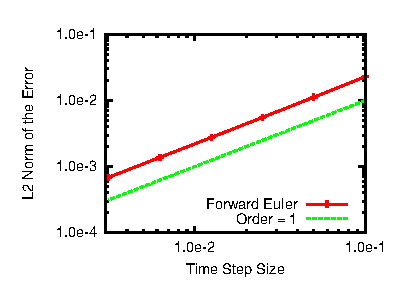
\includegraphics[scale=1.5]{figures/ForwardEuler}\caption{Order of accuracy for the SinCos Problem (Section~\ref{rythmos:sec:SinCos-Problem})
using Forward Euler.\label{rythmos:fig:OrderofAccuracy-ForwardEuler}}
\end{figure}



\subsection{Explicit Runge-Kutta Methods\label{rythmos:sec:Explicit-Runge-Kutta-Methods}}

The general Runge-Kutta method for $s$-stages, can be written as
\[
X_{i}=x_{n-1}+\Delta t\,\sum_{j=1}^{s}a_{ij}\,\bar{f}(X_{j},t_{n-1}+c_{j}\Delta t)
\]
\[
x_{n}=x_{n-1}+\Delta t\,\sum_{i=1}^{s}b_{i}\,\bar{f}(X_{i},t_{n-1}+c_{i}\Delta t)
\]
where $X_{i}$ are intermediate approximations to the solution at
times, $t_{n-1}+c_{i}\Delta t$, (\emph{stage solutions}) which may
be correct to a lower order of accuracy than the solution, $x_{n}$.
We should note that these lower-order approximations are combined
through $b_{i}$ so that error terms cancel out and produce a more
accurate solution \cite[p. 80]{AscherPetzold}. One can also write
this in terms of $\dot{X}_{i}$ (or $\bar{f}(x,t)$)
\[
\dot{X}_{i}=\bar{f}\left(x_{n-1}+\Delta t\,\sum_{j=1}^{s}a_{ij}\,\dot{X}_{j},t_{n-1}+c_{i}\Delta t\right)
\]
\[
x_{n}=x_{n-1}+\Delta t\,\sum_{i=1}^{s}b_{i}\,\dot{X}_{i}
\]


A convenient method to convey Runge-Kutta methods is to use the Butcher
Tableau, which displays the coefficients in a ``table'' form.
\begin{table}[H]
\caption{Schematic for a Butcher Tableau.\label{rythmos:tab:SchematicButcherTableau}}
\[
\begin{array}{c|cccc}
c_{1} & a_{11} & a_{12} & \ldots & a_{1s}\\
c_{2} & a_{21} & a_{22} & \ldots & a_{2s}\\
\vdots & \vdots & \vdots & \ddots & \vdots\\
c_{s} & a_{s1} & a_{s2} & \ldots & a_{ss}\\
\hline  & b_{1} & b_{2} & \ldots & b_{s}
\end{array}
\]
\end{table}
Notes:
\begin{enumerate}
\item $c_{i}$ is the fractional time step that the approximate solution
$X_{i}$ is known. It is possible for $c_{i}$ to be outside the time
step range {[}0,1{]}, however it is odd for a One-Step methods like
Runge-Kutta to have stage solutions outside the current time step. 
\item $c_{i}=\sum_{j=1}^{s}a_{ij}$ for $i=1,\ldots,s$
\item For explicit methods, \emph{e.g.}, Forward Euler and Explicit RK4,
$c_{1}=0$ and $a_{1j}=0$ for all $j$ indicates that one needs the
solution, $x_{n-1}$, and its time derivative, $\dot{x}_{n-1}$, (or
basically an evaluation of $\bar{f}(x_{n-1},t_{n-1})$) to start the
time step.
\item If $a_{ij}=0$ for $j\ge i$, the Runge-Kutta (RK) method is explicit
(also known as ERK), since each $X_{i}$ is given in terms of known
quantities.
\item If $a_{ij}\ne0$ for any $j\ge i$, the Runge-Kutta (RK) method is
implicit (also known as IRK), since an implicit solve is required
for at least some of the stages.
\item If $a_{ij}=0$ for $j>i$, the method is known as a Diagonally Implicit
Runge-Kutta (DIRK) method. DIRK methods require an implicit solution
for each stage, but are not coupled to other stages.
\item If $a_{ij}=0$ for $j>i$ and $a_{ii}=C$, the method is known as
a Singly Diagonally Implicit Runge-Kutta (SDIRK) method. Like with
DIRK methods, an implicit solve is needed at each stage, but since
$a_{ii}$ is the same, some of the preportory calculations can be
reused for each stage.
\item $b_{i}$ are the weighting of the intermediate solutions, $X_{i}$,
to obtain the final solution, and they are a partition of unity, $\sum_{i=1}^{s}b_{i}=1$.
\item If $a_{sj}=b_{j}$ for all $j$ or $a_{i1}=b_{1}$ for all $i$, and
$a_{ij}$ is a nonsingular matrix, then A-stable RK methods are L-stable
\cite[p. 45]{HairerWanner}\cite[p. 103]{AscherPetzold}, \emph{e.g.},
Backward Euler and two SDIRK methods. Each of the above conditions
are not a necessary condition for L-stability, but they are a sufficient
condition.
\end{enumerate}

\subsection{Explicit RK Forward Euler}

Forward Euler can also be written for Runge-Kutta methods, Fig.~\ref{rythmos:fig:ERK-ForwardEuler},
and obtains convergence results similar to Forward Euler, Section~\ref{rythmos:sec:Forward-Euler}.
\begin{figure}[H]
\centering{}%
\begin{tabular}{cc}
a)$\begin{array}{c|c}
0 & 0\\
\hline  & 1
\end{array}$ & b)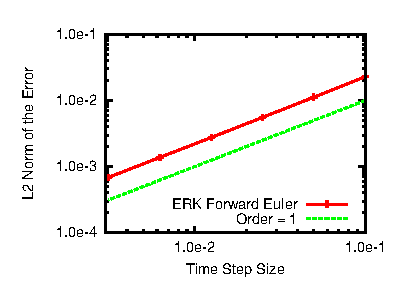
\includegraphics[scale=1.5]{figures/ERK_ForwardEuler}\tabularnewline
\end{tabular}\caption{a) Butcher Tableau and b) Order of accuracy for the SinCos Problem
(Section~\ref{rythmos:sec:SinCos-Problem}) for Explicit RK Forward
Euler.\label{rythmos:fig:ERK-ForwardEuler}}
\end{figure}



\subsection{Explicit RK 2 Stage 2 Order by Runge (Explicit Midpoint)}

\begin{figure}[H]
\centering{}%
\begin{tabular}{cc}
a) $\begin{array}{c|cc}
0 & 0\\
1/2 & 1/2 & 0\\
\hline  & 0 & 1
\end{array}$ & b)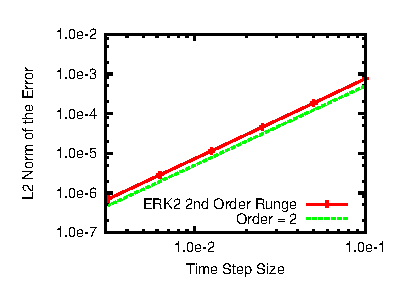
\includegraphics[scale=1.5]{figures/ERK_2Stage2OrderRunge}\tabularnewline
\end{tabular}\caption{a) Butcher Tableau and b) Order of accuracy for the SinCos Problem
(Section~\ref{rythmos:sec:SinCos-Problem}) for Explicit RK 2 Stage
2nd Order by Runge.\label{rythmos:tab:ButcherTableau-ERK_2Stage2OrderRunge}.}
\end{figure}



\subsection{Explicit RK Trapezoidal}

\begin{figure}[H]
\centering{}%
\begin{tabular}{cc}
a) $\begin{array}{c|cc}
0 & 0\\
1 & 1 & 0\\
\hline  & 1/2 & 1/2
\end{array}$ & b)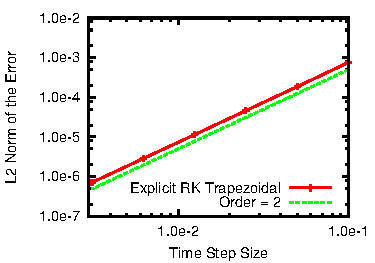
\includegraphics[scale=1.5]{figures/ERK_Trapezoidal}\tabularnewline
\end{tabular}\caption{a) Butcher Tableau and b) Order of accuracy for the SinCos Problem
(Section~\ref{rythmos:sec:SinCos-Problem}) for Explicit RK Trapezoidal.\label{rythmos:tab:ButcherTableau-ERK_Trapezoidal}}
\end{figure}



\subsection{Explicit RK 3 Stage 3 Order}

\begin{figure}[H]
\centering{}%
\begin{tabular}{cc}
a)$\begin{array}{c|ccc}
0 & 0\\
1/2 & 1/2 & 0\\
1 & -1 & 2 & 0\\
\hline  & 1/6 & 4/6 & 1/6
\end{array}$ & b)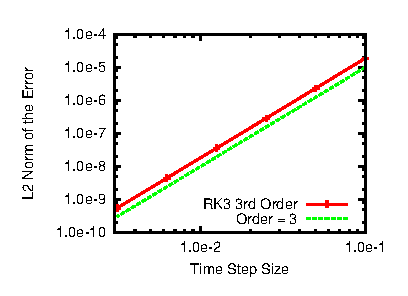
\includegraphics[scale=1.5]{figures/ERK_3Stage3Order}\tabularnewline
\end{tabular}\caption{a) Butcher Tableau and b) Order of accuracy for the SinCos Problem
(Section~\ref{rythmos:sec:SinCos-Problem}) for Explicit RK 3 Stage
3rd Order.\label{rythmos:tab:ButcherTableau-ERK_3Stage3Order}}
\end{figure}



\subsection{Explicit RK 3 Stage 3 Order by Heun}

\begin{figure}[H]
\centering{}%
\begin{tabular}{cc}
a) $\begin{array}{c|ccc}
0 & 0\\
1/3 & 1/3 & 0\\
2/3 & 0 & 2/3 & 0\\
\hline  & 1/4 & 0 & 3/4
\end{array}$ & b)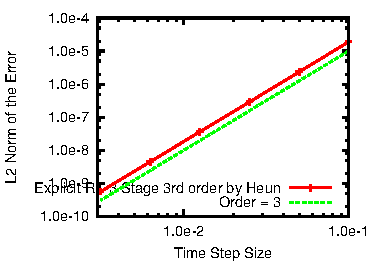
\includegraphics[scale=1.5]{figures/ERK_3Stage3OrderHeun}\tabularnewline
\end{tabular}\caption{a) Butcher Tableau and b) Order of accuracy for the SinCos Problem
(Section~\ref{rythmos:sec:SinCos-Problem}) for Explicit RK 3 Stage
3rd Order by Heun.\label{rythmos:tab:ButcherTableau-ERK_3Stage3OrderHeun}}
\end{figure}



\subsection{Explicit RK 3 Stage 3 Order TVD}

\begin{figure}[H]
\centering{}%
\begin{tabular}{cc}
a)$\begin{array}{c|ccc}
0 & 0\\
1 & 1 & 0\\
1/2 & 1/4 & 1/4 & 0\\
\hline  & 1/6 & 1/6 & 4/6
\end{array}$ & b)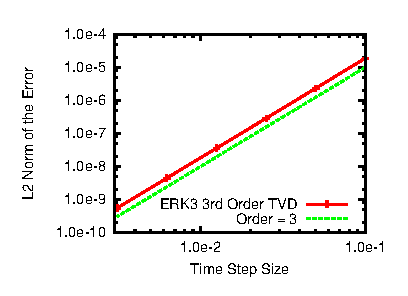
\includegraphics[scale=1.5]{figures/ERK_3Stage3OrderTVD}\tabularnewline
\end{tabular}\caption{a) Butcher Tableau and b) Order of accuracy for the SinCos Problem
(Section~\ref{rythmos:sec:SinCos-Problem}) for Explicit RK 3 Stage
3rd Order TVD.\label{rythmos:tab:ButcherTableau-ERK_3Stage3OrderTVD}}
\end{figure}



\subsection{Explicit RK 4 Stage 3 Order by Runge}

\begin{figure}[H]
\centering{}%
\begin{tabular}{cc}
a)$\begin{array}{c|cccc}
0 & 0\\
1/2 & 1/2 & 0\\
1 & 0 & 1 & 0\\
1 &  & 0 & 1 & 0\\
\hline  & 1/6 & 2/3 & 0 & 1/6
\end{array}$ & b)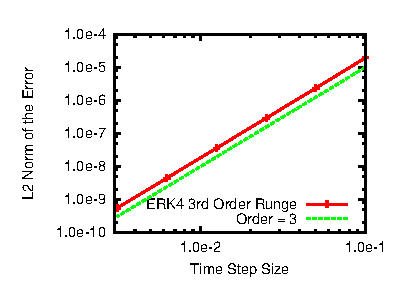
\includegraphics[scale=1.5]{figures/ERK_4Stage3OrderRunge}\tabularnewline
\end{tabular}\caption{a) Butcher Tableau and b) Order of accuracy for the SinCos Problem
(Section~\ref{rythmos:sec:SinCos-Problem}) for Explicit RK 4 Stage
3rd Order by Runge.\label{rythmos:tab:ButcherTableau-ERK_4Stage3OrderRunge}}
\end{figure}



\subsection{Explicit RK4}

\begin{figure}[H]
\centering{}%
\begin{tabular}{cc}
a)$\begin{array}{c|cccc}
0 & 0\\
1/2 & 1/2 & 0\\
1/2 & 0 & 1/2 & 0\\
1 & 0 & 0 & 1 & 0\\
\hline  & 1/6 & 1/3 & 1/3 & 1/6
\end{array}$ & b)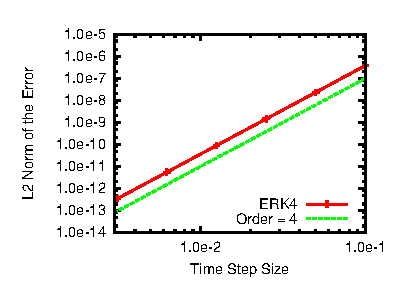
\includegraphics[scale=1.5]{figures/ERK_4Stage}\tabularnewline
\end{tabular}\caption{a) Butcher Tableau and b) Order of accuracy for the SinCos Problem
(Section~\ref{rythmos:sec:SinCos-Problem}) for Explicit RK 4.\label{rythmos:tab:ButcherTableau-ERK_4Stage}.}
\end{figure}



\subsection{Explicit RK 3/8 Rule}

\begin{figure}[H]
\centering{}%
\begin{tabular}{cc}
a)$\begin{array}{c|cccc}
0 & 0\\
1/3 & 1/3 & 0\\
2/3 & -1/3 & 1 & 0\\
1 & 1 & -1 & 1 & 0\\
\hline  & 1/8 & 3/8 & 3/8 & 1/8
\end{array}$ & b)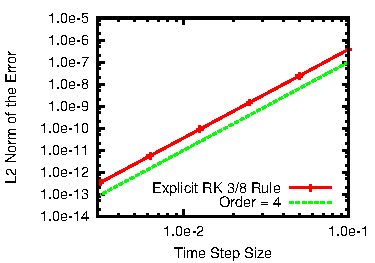
\includegraphics[scale=1.5]{figures/ERK_3_8_Rule}\tabularnewline
\end{tabular}\caption{a) Butcher Tableau and b) Order of accuracy for the SinCos Problem
(Section~\ref{rythmos:sec:SinCos-Problem}) for Explicit RK 3/8 Rule.\label{rythmos:tab:ButcherTableau-ERK_3_8_Rule}}
\end{figure}


\section{Formulation for Implicit Time Steppers for ODEs and DAEs}

\label{rythmos:sec:implicit-time-steppers}

Here we consider several different classes of implicit time stepping
methods. For each class of method we show the set of general nonlinear
equations that defines a single time step and then show how a linearized
form of the equations may be formed to be solved by a Newton-type
nonlinear equation solver.

In particular, for each method, we will show how to define a set of
nonlinear equations of the form 
\begin{equation}
r(z)=0\label{rythmos:eq:r}
\end{equation}
such that when solved will define an implicit time step from $t_{k}$
to $t_{k+1}$, where $\Delta t=t_{k+1}-t_{k}$ denotes the time-step.
In addition, for each method, we will show how to use the DAE residual
evaluation $(\dot{x},x,t){}\rightarrow f$ to define the nonlinear
time step equation (\ref{rythmos:eq:r}). At the highest level, the
time step method only requires very general convergence criteria for
the time step equation (\ref{rythmos:eq:r}) and therefore great flexibility
is allowed in how the time step equation is solved. In general, the
system in (\ref{rythmos:eq:r}) must be solved such that $||x_{k+1}-x^{*}(t_{k+1})||<\eta$,
where $x_{k+1}\in\mathcal{X}$ is the computed step for the state,
$x^{*}(t_{k+1})\in\mathcal{X}$ is the exact state solution at $t_{k+1}$,
and $\eta$ is the maximum allowable local truncation error defined
by the user.

Even though the time step equation can be solved by a variety of means,
a large class of DAEs can also potentially provide support for a general
Newton-type method for solving these equations and can therefore leverage
general software for solving such problems (e.g.\ NOX). The foundation
of Newton-like methods is the ability to solve linear systems similar
to the Newton system 
\begin{equation}
\Jac{r}{z}\Delta z=-r(z_{l})
\end{equation}
where $z_{l}$ is the current candidate solution of the nonlinear
equations (which also defines the point where $\jac{r}{z}$ is evaluated)
and $\Delta z=r_{l+1}-r_{l}$ is the update direction. Line-search
Newton methods then define an update to the solution along the direction
$\Delta z$. The essential functionality needed to perform a Newton-like
method are the the abilities to evaluate the nonlinear residual $z{}\rightarrow r$
and to (approximately) solve linear systems involving the Jacobian
matrix $\jac{r}{z}$. For each type of implicit time integration method,
we will show, if possible, how to perform solves with $\jac{r}{z}$
by performing solves with the matrix 
\begin{equation}
W=\alpha\Jac{f}{\dot{x}}+\beta\Jac{f}{x},\label{rythmos:eq:W}
\end{equation}
evaluated at points $(\dot{x},x,t)$ selected by the time integration
method and where $\alpha\in\RE$ and $\beta\in\RE$ is some constants
also defined by the time integration method. Note that the matrix
$W$ above in (\ref{rythmos:eq:W_bdf}) may not necessarily exactly
represent $\jac{r}{z}$ and $z$ and $r$ may not simply lie in the
vector spaces $\mathcal{X}$ and $\mathcal{F}$ respectively; but
in many cases, they will.

The iteration matrix, $W$, is defined to be
\[
W\equiv\frac{df}{dx_{n}}=\frac{\partial\dot{x}}{\partial x_{n}}\Jac{f}{\dot{x}}+\frac{\partial x}{\partial x_{n}}\Jac{f}{x}=\alpha\Jac{f}{\dot{x}}+\beta\Jac{f}{x}
\]
where $\alpha=\partial\dot{x}/\partial x_{n}$ and $\beta=\partial x/\partial x_{n}$,
and recalling $f\left(\dot{x}(x_{n}),x(x_{n})\right)=0$.


\subsection{Backward Euler}


\subsubsection{Constant Step Size}

In Fig.~\ref{rythmos:fig:BackwardEuler-Constant-dt}, the order of
accuracy is shown for Backward Euler for the SinCos problem.

\begin{figure}[H]
\centering{}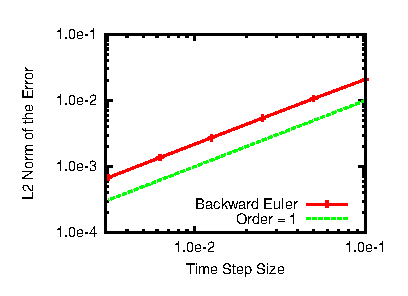
\includegraphics[scale=1.5]{figures/BackwardEuler}\caption{Order of accuracy for the SinCos Problem (Section~\ref{rythmos:sec:SinCos-Problem})
using Backward Euler.\label{rythmos:fig:BackwardEuler-Constant-dt}}
\end{figure}



\subsubsection{Variable Step Size}

A good test for variable step size is the Log-Time problem which is
defined in Sec.~\ref{rythmos:sec:Log-Time-Problem}. To adjust the
step size, the FirstOrderErrorStepControlStrategy uses the difference
between the predicted and final solution as an measure of the temporal
error and sets the next step size to maintain the user specified level
of error. Figure~\ref{rythmos:fig:BackwardEuler-Variable-dt} shows
this for the Backward Euler method for four different relative errors,
$\epsilon_{r}=$ $10^{-2}$, $10^{-3}$, $10^{-4}$, and $10^{-5}$. 

\begin{figure}[H]
\centering{}%
\begin{tabular}{cc}
a)\includegraphics[width=2.75in]{figures/BackwardEuler_FirstOrderError_var_dt_RelError=1\lyxdot 0e-2} & b)\includegraphics[width=2.75in]{figures/BackwardEuler_FirstOrderError_var_dt_RelError=1\lyxdot 0e-3}\tabularnewline
c)\includegraphics[width=2.75in]{figures/BackwardEuler_FirstOrderError_var_dt_RelError=1\lyxdot 0e-4} & d)\includegraphics[width=2.75in]{figures/BackwardEuler_FirstOrderError_var_dt_RelError=1\lyxdot 0e-5}\tabularnewline
\end{tabular}\caption{Solution and time step sizes for the Log-Time Problem (Section~\ref{rythmos:sec:Log-Time-Problem})
using Backward Euler with various relative errors in the FirstOrderErrorStepControlStrategy:
a) $\epsilon_{r}=$ a) $10^{-2}$, b) $10^{-3}$, c) $10^{-4}$, and
d) $10^{-5}$.\label{rythmos:fig:BackwardEuler-Variable-dt}}
\end{figure}


In Table~\ref{rythmos:tab:BackwardEuler-Variable-dt-Log-Time}, the
errors for this problem are shown. For each magnitude reduction in
the relative-error specification, the number of steps increases by
a factor of 2-3 and a similar reduction in the error norms and global
errors.

\begin{table}


\begin{centering}
\caption{Log-Time Errors for Backward Euler with Variable Step Size for the
Log-Time Problem.\label{rythmos:tab:BackwardEuler-Variable-dt-Log-Time}}
\begin{tabular}{|c|c|c|c|}
\hline 
$\epsilon_{r}$ & Number of Steps & Error Norm ($0\leq t_{n}\leq1$) & Global Error ($t=1$)\tabularnewline
\hline 
\hline 
$10^{-2}$ & 213 & 0.0224098 & 0.0224576\tabularnewline
\hline 
$10^{-3}$ & 563 & 0.0132322 & 0.0132634\tabularnewline
\hline 
$10^{-4}$ & 1534 & 0.00480765 & 0.00482358\tabularnewline
\hline 
$10^{-5}$ & 4168 & 0.00153523 & 0.00154173\tabularnewline
\hline 
\end{tabular}
\par\end{centering}

\end{table}


The exponential growth in the time step size, $\Delta t$, over $10^{-8}<t<1$
is approximately 8\% ($\Delta t_{n}\approx1.08\Delta t_{n-1}$), which
doubles the step size approximately every 10 time steps, and is unaffected
by the relative error, $\epsilon_{r}$. The primary effect of $\epsilon_{r}$
is to reduce $\Delta t$ over the majority of the run, except for
the initial few steps (\textasciitilde{}10). The two `blips' near
$t=10^{-9}$ are evident with all $\epsilon_{r}$, and correspond
to the locations where the curvature in the solution are large.
\include{RythmosTheoryBDF}
\subsection{Implicit Runge-Kutta methods\label{rythmos:sec:Implicit-Runge-Kutta-methods}}

We now consider a class of powerful and popular one-step methods for
solving implicit DAEs, implicit Runge-Kutta (RK) methods. The most
general form of implicit RK methods requires the simultaneous solution
of $s$ sets of coupled nonlinear equations that take the form
\begin{equation}
r_{i}(z)=f\left(\dot{X}_{i},\; x_{n-1}+\Delta t\,\sum_{j=1}^{s}a_{ij}\,\dot{X}_{j},\; t_{n-1}+c_{i}\Delta t\right)=0\label{rythmos:eqn:irk_dae_ne}
\end{equation}
for $i=1,\ldots,s$ where $\dot{X}_{i}$ are essentially approximations
to the derivatives $\dot{x}(t_{n-1}+c_{i}\Delta t)$ called \emph{stage
derivatives} and $z=[\dot{X}_{1},\dot{X}_{2},\ldots,\dot{X}_{s}]^{T}$
are the unknowns in this set of equations. After this set of coupled
equations is solved, the state solution $x_{n}$ is given as the linear
combination
\[
x_{n}=x_{n-1}+\Delta t\,\sum_{i=1}^{s}b_{i}\,\dot{X}_{i}
\]
It is clear how to form the residual for the fully coupled system
for $r(z)$ in Eq.~(\ref{rythmos:eqn:irk_dae_ne}) just from individual
evaluations. How the Newton system for such a system is solved will
vary greatly based on the structure and properties of the Butcher
matrix, $a_{ij}$. 

Fully implicit RK methods present somewhat of a problem for developing
general software since they involve the need to solve a fully coupled
system of $s$ sets of equations of the form of Eq.~(\ref{rythmos:eqn:irk_dae_ne}).
Each block $\jac{r_{i}}{z_{j}}=\jac{r_{i}}{\dot{X}_{j}}$ of the full
Jacobian $\jac{r}{z}$ is represented as 
\begin{eqnarray}
W_{ij} & = & \alpha\Jac{f}{\dot{x}}+\beta\Jac{f}{x}\nonumber \\
 & = & \Jac{r_{i}}{z_{j}}=\Jac{r_{i}}{\dot{X}_{j}}\nonumber \\
 & = & \frac{\partial\dot{x}}{\partial\dot{X}_{j}}\Jac{f}{\dot{x}}+\frac{\partial x}{\partial\dot{X}_{j}}\Jac{f}{x}\nonumber \\
 & = & \delta_{ij}\Jac{f}{\dot{x}}+\Delta t\, a_{ij}\Jac{f}{x}\label{rythmos:eq:dridzj_IRK}
\end{eqnarray}
for $i=1,\ldots,s$ and $j=1,\ldots,s$ which is evaluated at the
points $(\dot{x},x,t)=(\dot{X}_{i},\;$ $x_{n-1}+\Delta t\,\sum_{j=1}^{s}a_{ij}\,\dot{X}_{j},\;$
$t_{n-1}+c_{i}\Delta t)$. Note that the iteration matrix, $W$, has
$\alpha=\delta_{ij}$ and $\beta=\Delta t\, a_{ij}$.

When considering a iterative method for solving systems with the block
operator matrix $\jac{r}{z}$, it is easy to see how to use the iteration
matrix $W$ in Eq.~(\ref{rythmos:eq:W}) to implement a matrix-vector
product, but it is not obvious how to precondition such a system.
Clearly a block diagonal preconditioner could be used but the effectiveness
of such a preconditioning strategy is open to question. Other preconditioning
strategies are also possible just given the basic block operators
and this is an open area of research. In some cases, however, it may
be possible to form a full matrix object for $\jac{r}{z}$ but this
is not something that can be expected for most applications.


\paragraph{Semi-explicit IRK methods}

Semi-explicit IRK methods are those IRK methods where the Butcher
matrix, $A$, is lower diagonal and therefore gives rise to a block
lower triangular Jacobian matrix $\jac{r}{z}$. For these types of
methods, the nonlinear equations in Eq.~(\ref{rythmos:eq:dridzj_IRK})
can be solved one at a time for $i=1,\ldots,s$ which is easily accommodated
using a Newton-type method where the Newton Jacobian for each $i$
is given by Eq.~(\ref{rythmos:eq:dridzj_IRK}), which is of our basic
general form, Eq.~(\ref{rythmos:eq:W}).


\paragraph{Singly-Diagonal-implicit IRK methods}

The next specialized class of IRK methods that we consider are singly-diagonal-implicit
IRK methods where the Butcher coefficients in $a_{ij}$ and $c$ give
rise to a lower triangular Jacobian $\jac{r}{z}$ (and hence are also
semi-explicit IRK methods) that has the same nonsingular matrix block
of the form in Eq.~(\ref{rythmos:eq:dridzj_IRK}) along the diagonal.
This, of course, requires that $a_{11}=a_{22}=\cdots=a_{ss}$ and
$c_{1}=c_{2}=\cdots=c_{s}$. (I am not sure that this is possible,
since $c_{i}=\sum_{j=1}^{s}a_{ij}$. The only method that satisfies
this is IRK Backward Euler!? CCO) In this class of IRK methods, significant
savings may be achieved since a single set of linear solver objects
(\emph{i.e.}, operators and preconditioners) can be utilized for the
solution of the fully coupled system. In fact, it may even be possible
to utilize multi-vector applications of the operator and preconditioner
for matrices of the form Eq.~(\ref{rythmos:eq:W}) which can be supported
by many applications. 


\subsubsection{Implicit RK Backward Euler}

\begin{figure}[H]
\centering{}%
\begin{tabular}{cc}
a) $\begin{array}{c|c}
1 & 1\\
\hline  & 1
\end{array}$ & b)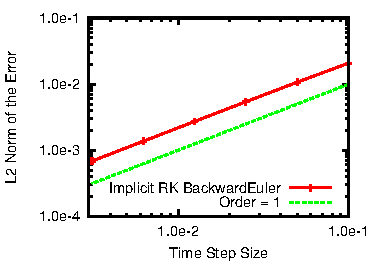
\includegraphics[scale=1.5]{figures/IRK_BackwardEuler}\tabularnewline
\end{tabular}\caption{a) Butcher Tableau and b) Order of accuracy for the SinCos Problem
(Section~\ref{rythmos:sec:SinCos-Problem}) for Implicit RK Backward
Euler.}
\end{figure}



\subsubsection{IRK 1 Stage Theta}

This is a generalization of the midpoint method ($\theta=1/2$).

\begin{figure}[H]
\centering{}%
\begin{tabular}{cc}
a) $\begin{array}{c|c}
\theta & \theta\\
\hline  & 1
\end{array}$ & b)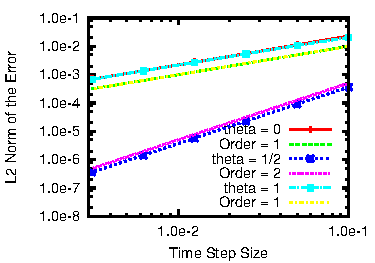
\includegraphics[scale=1.5]{figures/IRK1StageTheta1}\tabularnewline
\end{tabular}\caption{a) Butcher Tableau and b) Order of accuracy for the SinCos Problem
(Section~\ref{rythmos:sec:SinCos-Problem}) for IRK 1 Stage Theta
method.}
\end{figure}



\subsubsection{IRK 2 Stage Theta}

This is a generalization of the trapezoid method ($\theta=1/2$).

\begin{figure}[H]
\centering{}%
\begin{tabular}{cc}
a) $\begin{array}{c|cc}
0 & 0\\
1 & 1-\theta & \theta\\
\hline  & 1-\theta & \theta
\end{array}$ & b)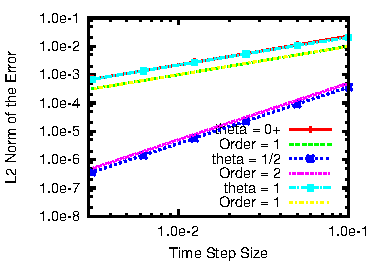
\includegraphics[scale=1.5]{figures/IRK2StageTheta1}\tabularnewline
\end{tabular}\caption{a) Butcher Tableau and b) Order of accuracy for the SinCos Problem
(Section~\ref{rythmos:sec:SinCos-Problem}) for IRK 2 Stage Theta
method.}
\end{figure}



\subsubsection{SDIRK 2 Stage 2 Order}

For $\gamma=(2\pm\sqrt{2})/2$, this method is 2nd order accurate
and L-stable. Other values of $\gamma$ will still produce an L-stable
scheme, but with only be 1st order accurate.

\begin{figure}[H]
\centering{}%
\begin{tabular}{cc}
a) $\begin{array}{c|cc}
\gamma & \gamma\\
1 & 1-\gamma & \gamma\\
\hline  & 1-\gamma & \gamma
\end{array}$ & b)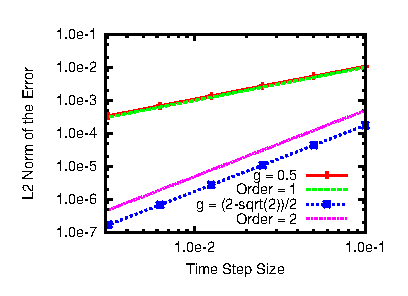
\includegraphics[scale=1.5]{figures/SDIRK_2Stage2Order}\tabularnewline
\end{tabular}\caption{a) Butcher Tableau and b) Order of accuracy for the SinCos Problem
(Section~\ref{rythmos:sec:SinCos-Problem}) for SDIRK 2 Stage 2 Order.}
\end{figure}



\subsubsection{SDIRK 2 Stage 3 Order}

For $\gamma=(3\pm\sqrt{3})/6$, this method is 3rd order accurate
and A-stable. For $\gamma=(2\pm\sqrt{2})/2$, this method is only
2nd order accurate, but is then L-stable.

\begin{figure}[H]
\centering{}%
\begin{tabular}{cc}
a) $\begin{array}{c|cc}
\gamma & \gamma\\
1-\gamma & 1-2\gamma & \gamma\\
\hline  & 1/2 & 1/2
\end{array}$ & b)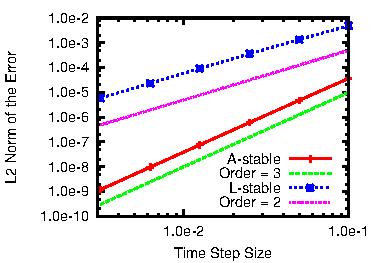
\includegraphics[scale=1.5]{figures/SDIRK_2Stage3OrderLStable}\tabularnewline
\end{tabular}\caption{a) Butcher Tableau and b) Order of accuracy for the SinCos Problem
(Section~\ref{rythmos:sec:SinCos-Problem}) for SDIRK 2 Stage 3 Order.}
\end{figure}



\subsubsection{SDIRK 3 Stage 4 Order}

The coefficients are $\gamma=1/\sqrt{3}\,\cos(\pi/18)+1/2$ and $\delta=(2\gamma-1)^{-2}/6$.

\begin{figure}[H]
\centering{}%
\begin{tabular}{cc}
a)$\begin{array}{c|ccc}
\gamma & \gamma\\
1/2 & 1/2-\gamma & \gamma\\
1-\gamma & 2\gamma & 1-4\gamma & \gamma\\
\hline  & \delta & 1-2\delta & \delta
\end{array}$ & b)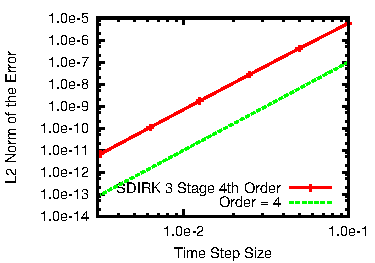
\includegraphics[scale=1.5]{figures/SDIRK_3Stage4Order}\tabularnewline
\end{tabular}\caption{a) Butcher Tableau and b) Order of accuracy for the SinCos Problem
(Section~\ref{rythmos:sec:SinCos-Problem}) for SDIRK 3 Stage 4 Order.}
\end{figure}



\subsubsection{SDIRK 5 Stage 4 Order}

\begin{figure}[H]
\centering{}$\begin{array}{c|ccccc}
1/4 & 1/4\\
3/4 & 1/2 & 1/4\\
11/20 & 17/50 & -1/25 & 1/4\\
1/2 & 371/1360 & -137/2720 & 15/544 & 1/4\\
1 & 25/24 & -49/48 & 125/16 & -85/12 & 1/4\\
\hline  & 25/24 & -49/48 & 125/16 & -85/12 & 1/4\\
 & 59/48 & -17/96 & 225/32 & -85/12 & 0
\end{array}$\caption{Butcher Tableau for SDIRK 5 Stage 4 Order.}
\end{figure}
\begin{figure}[H]
\centering{}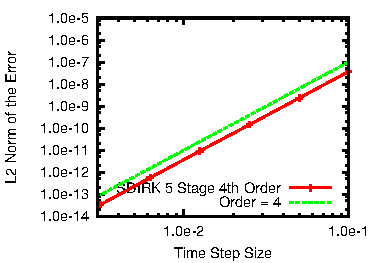
\includegraphics[scale=1.5]{figures/SDIRK_5Stage4Order}\caption{Order of accuracy for the SinCos Problem (Section~\ref{rythmos:sec:SinCos-Problem})
using SDIRK 5 Stage 4 Order.}
\end{figure}



\subsubsection{SDIRK 5 Stage 5 Order}

\begin{figure}[H]
\centering{}$\begin{array}{c|ccccc}
\frac{6-\sqrt{6}}{10} & \frac{6-\sqrt{6}}{10}\\
\frac{6+\sqrt{6}}{35} & \frac{-6+5\sqrt{6}}{14} & \frac{6-\sqrt{6}}{10}\\
1 & \frac{888+607\sqrt{6}}{2850} & \frac{126-161\sqrt{6}}{1425} & \frac{6-\sqrt{6}}{10}\\
\frac{4-\sqrt{6}}{10} & \frac{3153-3082\sqrt{6}}{14250} & \frac{3213+1148\sqrt{6}}{28500} & \frac{-267+88\sqrt{6}}{500} & \frac{6-\sqrt{6}}{10}\\
\frac{4+\sqrt{6}}{10} & \frac{-32583+14638\sqrt{6}}{71250} & \frac{-17199+364\sqrt{6}}{142500} & \frac{1329-544\sqrt{6}}{2500} & \frac{-96+131\sqrt{6}}{625} & \frac{6-\sqrt{6}}{10}\\
\hline  & 0 & 0 & 1/9 & \frac{16-\sqrt{6}}{36} & \frac{16+\sqrt{6}}{36}
\end{array}$\caption{Butcher Tableau for SDIRK 5 Stage 5 Order.}
\end{figure}
\begin{figure}[H]
\centering{}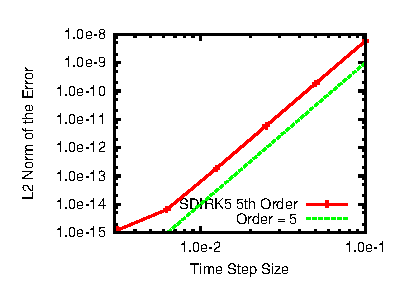
\includegraphics[scale=1.5]{figures/SDIRK_5Stage5Order}\caption{Order of accuracy for the SinCos Problem (Section~\ref{rythmos:sec:SinCos-Problem})
for SDIRK 5 Stage 5 Order.}
\end{figure}



\subsubsection{DIRK 2 Stage 3 Order}

\begin{figure}[H]
\centering{}%
\begin{tabular}{cc}
a)$\begin{array}{c|cc}
0 & 0\\
2/3 & 1/3 & 1/3\\
\hline  & 1/4 & 3/4
\end{array}$ & b)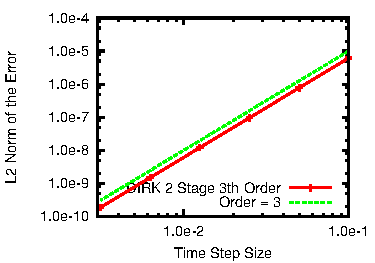
\includegraphics[scale=1.5]{figures/DIRK_2Stage3Order}\tabularnewline
\end{tabular}\caption{a) Butcher Tableau and b) Order of accuracy for the SinCos Problem
(Section~\ref{rythmos:sec:SinCos-Problem}) for DIRK 2 Stage 3 Order.}
\end{figure}



\newpage{}


\part{User's Manual}


\section{ParameterList Description}

The following description of the Rythmos ParameterList was auto-generated
from the ParameterList itself, thus allowing easy refreshing of the
input description and providing up-to-date information. Fig.~\ref{fig:ParameterList-schematic}
is a hyperlinked, indented heirarchy of the Rythmos ParameterList,
that provides an overall structure of the Rythmos ParameterList. The
hyerlinks are connected to subsequent sections, which contain additional
hyperlinks to parent and children sublists, and descriptions of the
sublist and parameters. All these hyperlinks provide an easy way to
hop around the parameters in order to setup the time-integrator. 

The basic structure starts with the ``Integrator Base'', and is
broken down into the Integrator and the Stepper. Each of these contain
several sublists giving the details of the Integrator and Stepper,
e.g., IntegrationControlStrategy, InterpolationBuffer, StepControlStrategy,
and error weight vector.

An easy way to create a Rythmos ParameterList is to get a valid ParameterList
from the IntegatorBuilder, and manipulate the parameters from there.
In this way, one able to correctly setup the Integrator and Stepper
for a transient soution. For example, \begin{verbatim}
  RCP<IntegratorBuilder<double> > ib = integratorBuilder<double>();
  RCP<ParameterList> pl = Teuchos::parameterList();
  pl->setParameters(*(ib->getValidParameters()));
  pl->sublist("Integrator Settings").set("Final Time", 1.0e-0);
\end{verbatim}

Obviously, most software will get its input specification from the
XML version of the ParameterLists, and then pass them onto Rythmos.
The description provided here can also help in setting up those XML
files. 

\begin{figure} 
\centering{} 
  \begin{tabular}{p{0.9\textwidth}}
\hspace*{0in} Integrator Base (Section~\ref{sec:Integrator Base})
    \index{Integrator Base} \\ 
\hspace*{0.2in} Integrator Settings (Section~\ref{sec:Integrator Settings})
    \index{Integrator Settings} \\ 
\hspace*{0.4in} Integrator Selection (Section~\ref{sec:Integrator Selection})
    \index{Integrator Selection} \\ 
\hspace*{0.6in} Default Integrator (Section~\ref{sec:Default Integrator})
    \index{Default Integrator} \\ 
\hspace*{0.8in} VerboseObject (Section~\ref{sec:VerboseObject})
    \index{VerboseObject} \\ 
\hspace*{0.2in} Integration Control Strategy Selection (Section~\ref{sec:Integration Control Strategy Selection})
    \index{Integration Control Strategy Selection} \\ 
\hspace*{0.4in} Simple Integration Control Strategy (Section~\ref{sec:Simple Integration Control Strategy})
    \index{Simple Integration Control Strategy} \\ 
\hspace*{0.4in} Ramping Integration Control Strategy (Section~\ref{sec:Ramping Integration Control Strategy})
    \index{Ramping Integration Control Strategy} \\ 
\hspace*{0.2in} Stepper Settings (Section~\ref{sec:Stepper Settings})
    \index{Stepper Settings} \\ 
\hspace*{0.4in} Stepper Selection (Section~\ref{sec:Stepper Selection})
    \index{Stepper Selection} \\ 
\hspace*{0.6in} Forward Euler (Section~\ref{sec:Forward Euler})
    \index{Forward Euler} \\ 
\hspace*{0.6in} Backward Euler (Section~\ref{sec:Backward Euler})
    \index{Backward Euler} \\ 
\hspace*{0.6in} Implicit BDF (Section~\ref{sec:Implicit BDF})
    \index{Implicit BDF} \\ 
\hspace*{0.6in} Explicit RK (Section~\ref{sec:Explicit RK})
    \index{Explicit RK} \\ 
\hspace*{0.6in} Implicit RK (Section~\ref{sec:Implicit RK})
    \index{Implicit RK} \\ 
\hspace*{0.4in} Step Control Settings (Section~\ref{sec:Step Control Settings})
    \index{Step Control Settings} \\ 
\hspace*{0.6in} Step Control Strategy Selection (Section~\ref{sec:Step Control Strategy Selection})
    \index{Step Control Strategy Selection} \\ 
\hspace*{0.8in} Fixed Step Control Strategy (Section~\ref{sec:Fixed Step Control Strategy})
    \index{Fixed Step Control Strategy} \\ 
\hspace*{0.8in} Simple Step Control Strategy (Section~\ref{sec:Simple Step Control Strategy})
    \index{Simple Step Control Strategy} \\ 
\hspace*{0.8in} First Order Error Step Control Strategy (Section~\ref{sec:First Order Error Step Control Strategy})
    \index{First Order Error Step Control Strategy} \\ 
\hspace*{0.8in} Implicit BDF Stepper Step Control Strategy (Section~\ref{sec:Implicit BDF Stepper Step Control Strategy})
    \index{Implicit BDF Stepper Step Control Strategy} \\ 
\hspace*{1in} magicNumbers (Section~\ref{sec:magicNumbers})
    \index{magicNumbers} \\ 
\hspace*{0.8in} Implicit BDF Stepper Ramping Step Control Strategy (Section~\ref{sec:Implicit BDF Stepper Ramping Step Control Strategy})
    \index{Implicit BDF Stepper Ramping Step Control Strategy} \\ 
\hspace*{0.6in} Error Weight Vector Calculator Selection (Section~\ref{sec:Error Weight Vector Calculator Selection})
    \index{Error Weight Vector Calculator Selection} \\ 
\hspace*{0.8in} Implicit BDF Stepper Error Weight Vector Calculator (Section~\ref{sec:Implicit BDF Stepper Error Weight Vector Calculator})
    \index{Implicit BDF Stepper Error Weight Vector Calculator} \\ 
\hspace*{0.4in} Interpolator Selection (Section~\ref{sec:Interpolator Selection})
    \index{Interpolator Selection} \\ 
\hspace*{0.6in} Linear Interpolator (Section~\ref{sec:Linear Interpolator})
    \index{Linear Interpolator} \\ 
\hspace*{0.6in} Hermite Interpolator (Section~\ref{sec:Hermite Interpolator})
    \index{Hermite Interpolator} \\ 
\hspace*{0.6in} Cubic Spline Interpolator (Section~\ref{sec:Cubic Spline Interpolator})
    \index{Cubic Spline Interpolator} \\ 
\hspace*{0.4in} Runge Kutta Butcher Tableau Selection (Section~\ref{sec:Runge Kutta Butcher Tableau Selection})
    \index{Runge Kutta Butcher Tableau Selection} \\ 
\hspace*{0.6in} Forward Euler (Section~\ref{sec:Forward Euler-Runge Kutta Butcher Tableau Selection})
    \index{Forward Euler} \\ 
\hspace*{0.6in} Explicit 2 Stage 2nd order by Runge (Section~\ref{sec:Explicit 2 Stage 2nd order by Runge})
    \index{Explicit 2 Stage 2nd order by Runge} \\ 
\hspace*{0.6in} Explicit Trapezoidal (Section~\ref{sec:Explicit Trapezoidal})
    \index{Explicit Trapezoidal} \\ 
\hspace*{0.6in} Explicit 3 Stage 3rd order (Section~\ref{sec:Explicit 3 Stage 3rd order})
    \index{Explicit 3 Stage 3rd order} \\ 
\hspace*{0.6in} Explicit 3 Stage 3rd order by Heun (Section~\ref{sec:Explicit 3 Stage 3rd order by Heun})
    \index{Explicit 3 Stage 3rd order by Heun} \\ 
\hspace*{0.6in}  ... \\ 
\hspace*{0.2in} Interpolation Buffer Settings (Section~\ref{sec:Interpolation Buffer Settings})
    \index{Interpolation Buffer Settings} \\ 
\hspace*{0.4in} Trailing Interpolation Buffer Selection (Section~\ref{sec:Trailing Interpolation Buffer Selection})
    \index{Trailing Interpolation Buffer Selection} \\ 
\hspace*{0.6in} Interpolation Buffer (Section~\ref{sec:Interpolation Buffer})
    \index{Interpolation Buffer} \\ 
\hspace*{0.4in} Interpolation Buffer Appender Selection (Section~\ref{sec:Interpolation Buffer Appender Selection})
    \index{Interpolation Buffer Appender Selection} \\ 
\hspace*{0.6in} Pointwise Interpolation Buffer Appender (Section~\ref{sec:Pointwise Interpolation Buffer Appender})
    \index{Pointwise Interpolation Buffer Appender} \\ 
\hspace*{0.4in} Interpolator Selection (Section~\ref{sec:Interpolator Selection-Interpolation Buffer Settings})
    \index{Interpolator Selection} \\ 
\hspace*{0.6in} Linear Interpolator (Section~\ref{sec:Linear Interpolator-Interpolator Selection})
    \index{Linear Interpolator} \\ 
\hspace*{0.6in} Hermite Interpolator (Section~\ref{sec:Hermite Interpolator-Interpolator Selection})
    \index{Hermite Interpolator} \\ 
\hspace*{0.6in} Cubic Spline Interpolator (Section~\ref{sec:Cubic Spline Interpolator-Interpolator Selection})
    \index{Cubic Spline Interpolator} \\ 
  \end{tabular}
\caption{Schematic of ParameterList heirarchy.} 
\label{fig:ParameterList-schematic} 
\end{figure} 
\newpage 

% ----------------------------------------------------------
\subsection{Integrator Base}
\label{sec:Integrator Base}
\index{Integrator Base}

\begin{list}{}
  {\setlength{\leftmargin}{1.0in}
   \setlength{\labelwidth}{0.75in}
   \setlength{\labelsep}{0.125in}}
  \item[Description:]
    The root ParameterList for the Integrator Builder.
  \item[Parent(s):]
   ROOT 
  \item[Child(ren):]
    Integrator Settings (Section~\ref{sec:Integrator Settings})
      \index{Integrator Settings} 
      \newline 
    Integration Control Strategy Selection (Section~\ref{sec:Integration Control Strategy Selection})
      \index{Integration Control Strategy Selection} 
      \newline 
    Stepper Settings (Section~\ref{sec:Stepper Settings})
      \index{Stepper Settings} 
      \newline 
    Interpolation Buffer Settings (Section~\ref{sec:Interpolation Buffer Settings})
      \index{Interpolation Buffer Settings} 
  \item[Parameters:]
    None. 
\end{list}

% ----------------------------------------------------------
\subsection{Integrator Settings}
\label{sec:Integrator Settings}
\index{Integrator Settings}

\begin{list}{}
  {\setlength{\leftmargin}{1.0in}
   \setlength{\labelwidth}{0.75in}
   \setlength{\labelsep}{0.125in}}
  \item[Description:]
    These parameters are used directly in setting up the Integrator.
  \item[Parent(s):]
    Integrator Base (Section~\ref{sec:Integrator Base})
      \index{Integrator Base} 
  \item[Child(ren):]
    Integrator Selection (Section~\ref{sec:Integrator Selection})
      \index{Integrator Selection} 
  \item[Parameters:]
    \begin{description}
      \item[Initial Time = 0] 
The initial time to start integration.
        \index{Integrator Settings!Initial Time}
        \index{Initial Time}
      \item[Final Time = 1] 
The final time to end integration.
        \index{Integrator Settings!Final Time}
        \index{Final Time}
      \item[Land On Final Time = 1] 
Exactly land on the final time; do not step past final time and interpolate.
        \index{Integrator Settings!Land On Final Time}
        \index{Land On Final Time}
\end{description}

\end{list}

% ----------------------------------------------------------
\subsection{Integrator Selection}
\label{sec:Integrator Selection}
\index{Integrator Selection}

\begin{list}{}
  {\setlength{\leftmargin}{1.0in}
   \setlength{\labelwidth}{0.75in}
   \setlength{\labelsep}{0.125in}}
  \item[Description:]
    Select the Integrator to be used.
  \item[Parent(s):]
    Integrator Settings (Section~\ref{sec:Integrator Settings})
      \index{Integrator Settings} 
  \item[Child(ren):]
    Default Integrator (Section~\ref{sec:Default Integrator})
      \index{Default Integrator} 
  \item[Parameters:]
    \begin{description}
      \item[Integrator Type = Default Integrator] 
Determines the type of Rythmos::Integrator object that will be built.
The parameters for each Integrator Type are specified in this sublist

  Valid std::string values:

      \begin{tabular}{lp{0.4\textwidth}}
      "None" & \\ 
      "Default Integrator" & \\ 
      \end{tabular}
        \index{Integrator Selection!Integrator Type}
        \index{Integrator Type}
\end{description}

\end{list}

% ----------------------------------------------------------
\subsection{Default Integrator}
\label{sec:Default Integrator}
\index{Default Integrator}

\begin{list}{}
  {\setlength{\leftmargin}{1.0in}
   \setlength{\labelwidth}{0.75in}
   \setlength{\labelsep}{0.125in}}
  \item[Description:]
    This Integrator will accept an IntergationControlStrategy, and can have an IntegrationObserver.  The client can specify the maximum number of time steps allowed.  The Integrator will loop over the Stepper until it reaches the requested time. For each step, the step size will be determined through a couple mechanisms/filters.  If an Integration Control Strategy has been specified, the step size and the step type (fixed or variable) will be determined by it.  Otherwise the step size will be set to the maximum real value and the step type will be variable.  Next if the step size is beyond the final time and the `Land On Final Time' is specified, the step size is adjusted to advance the state to the final time.  The Stepper is passed this step size and type to advance the state.  The DefaultIntegrator determines the step size and type taken by the Stepper, and if the step has failed.  If the IntegrationControlStrategy handles failures, it can suggest another step size and retry with the Stepper.  Otherwise, the Integrator will fall through with a failure.  With a successful step of the Stepper, the Integrator repeats the above until it reaches the requested time.  Multiple requested times can be passed to the Integrator.
  \item[Parent(s):]
    Integrator Selection (Section~\ref{sec:Integrator Selection})
      \index{Integrator Selection} 
  \item[Child(ren):]
    VerboseObject (Section~\ref{sec:VerboseObject})
      \index{VerboseObject} 
  \item[Parameters:]
    \begin{description}
      \item[Max Number Time Steps = 2147483647] 
Set the maximum number of integration time-steps allowed.
        \index{Default Integrator!Max Number Time Steps}
        \index{Max Number Time Steps}
\end{description}

\end{list}

% ----------------------------------------------------------
\subsection{VerboseObject}
\label{sec:VerboseObject}
\index{VerboseObject}

\begin{list}{}
  {\setlength{\leftmargin}{1.0in}
   \setlength{\labelwidth}{0.75in}
   \setlength{\labelsep}{0.125in}}
  \item[Description:]
  \item[Parent(s):]
    Default Integrator (Section~\ref{sec:Default Integrator})
      \index{Default Integrator} 
      \newline 
    Simple Integration Control Strategy (Section~\ref{sec:Simple Integration Control Strategy})
      \index{Simple Integration Control Strategy} 
      \newline 
    Ramping Integration Control Strategy (Section~\ref{sec:Ramping Integration Control Strategy})
      \index{Ramping Integration Control Strategy} 
      \newline 
    Forward Euler (Section~\ref{sec:Forward Euler})
      \index{Forward Euler} 
      \newline 
    Backward Euler (Section~\ref{sec:Backward Euler})
      \index{Backward Euler} 
      \newline 
    Implicit BDF (Section~\ref{sec:Implicit BDF})
      \index{Implicit BDF} 
      \newline 
    Explicit RK (Section~\ref{sec:Explicit RK})
      \index{Explicit RK} 
      \newline 
    Implicit RK (Section~\ref{sec:Implicit RK})
      \index{Implicit RK} 
      \newline 
    Fixed Step Control Strategy (Section~\ref{sec:Fixed Step Control Strategy})
      \index{Fixed Step Control Strategy} 
      \newline 
    Simple Step Control Strategy (Section~\ref{sec:Simple Step Control Strategy})
      \index{Simple Step Control Strategy} 
      \newline 
    First Order Error Step Control Strategy (Section~\ref{sec:First Order Error Step Control Strategy})
      \index{First Order Error Step Control Strategy} 
      \newline 
    magicNumbers (Section~\ref{sec:magicNumbers})
      \index{magicNumbers} 
      \newline 
    Implicit BDF Stepper Error Weight Vector Calculator (Section~\ref{sec:Implicit BDF Stepper Error Weight Vector Calculator})
      \index{Implicit BDF Stepper Error Weight Vector Calculator} 
      \newline 
    Linear Interpolator (Section~\ref{sec:Linear Interpolator})
      \index{Linear Interpolator} 
      \newline 
    Hermite Interpolator (Section~\ref{sec:Hermite Interpolator})
      \index{Hermite Interpolator} 
      \newline 
    Cubic Spline Interpolator (Section~\ref{sec:Cubic Spline Interpolator})
      \index{Cubic Spline Interpolator} 
      \newline 
    Forward Euler (Section~\ref{sec:Forward Euler-Runge Kutta Butcher Tableau Selection})
      \index{Forward Euler} 
      \newline 
    Explicit 2 Stage 2nd order by Runge (Section~\ref{sec:Explicit 2 Stage 2nd order by Runge})
      \index{Explicit 2 Stage 2nd order by Runge} 
      \newline 
    Explicit Trapezoidal (Section~\ref{sec:Explicit Trapezoidal})
      \index{Explicit Trapezoidal} 
      \newline 
    Explicit 3 Stage 3rd order (Section~\ref{sec:Explicit 3 Stage 3rd order})
      \index{Explicit 3 Stage 3rd order} 
      \newline 
    Explicit 3 Stage 3rd order by Heun (Section~\ref{sec:Explicit 3 Stage 3rd order by Heun})
      \index{Explicit 3 Stage 3rd order by Heun} 
      \newline 
    Explicit 3 Stage 3rd order TVD (Section~\ref{sec:Explicit 3 Stage 3rd order TVD})
      \index{Explicit 3 Stage 3rd order TVD} 
      \newline 
    Explicit 4 Stage 3rd order by Runge (Section~\ref{sec:Explicit 4 Stage 3rd order by Runge})
      \index{Explicit 4 Stage 3rd order by Runge} 
      \newline 
    Explicit 4 Stage (Section~\ref{sec:Explicit 4 Stage})
      \index{Explicit 4 Stage} 
      \newline 
    Explicit 3/8 Rule (Section~\ref{sec:Explicit 3/8 Rule})
      \index{Explicit 3/8 Rule} 
      \newline 
    Backward Euler (Section~\ref{sec:Backward Euler-Runge Kutta Butcher Tableau Selection})
      \index{Backward Euler} 
      \newline 
    IRK 1 Stage Theta Method (Section~\ref{sec:IRK 1 Stage Theta Method})
      \index{IRK 1 Stage Theta Method} 
      \newline 
    IRK 2 Stage Theta Method (Section~\ref{sec:IRK 2 Stage Theta Method})
      \index{IRK 2 Stage Theta Method} 
      \newline 
    Singly Diagonal IRK 2 Stage 2nd order (Section~\ref{sec:Singly Diagonal IRK 2 Stage 2nd order})
      \index{Singly Diagonal IRK 2 Stage 2nd order} 
      \newline 
    Singly Diagonal IRK 2 Stage 3rd order (Section~\ref{sec:Singly Diagonal IRK 2 Stage 3rd order})
      \index{Singly Diagonal IRK 2 Stage 3rd order} 
      \newline 
    Singly Diagonal IRK 3 Stage 4th order (Section~\ref{sec:Singly Diagonal IRK 3 Stage 4th order})
      \index{Singly Diagonal IRK 3 Stage 4th order} 
      \newline 
    Singly Diagonal IRK 5 Stage 4th order (Section~\ref{sec:Singly Diagonal IRK 5 Stage 4th order})
      \index{Singly Diagonal IRK 5 Stage 4th order} 
      \newline 
    Singly Diagonal IRK 5 Stage 5th order (Section~\ref{sec:Singly Diagonal IRK 5 Stage 5th order})
      \index{Singly Diagonal IRK 5 Stage 5th order} 
      \newline 
    Diagonal IRK 2 Stage 3rd order (Section~\ref{sec:Diagonal IRK 2 Stage 3rd order})
      \index{Diagonal IRK 2 Stage 3rd order} 
      \newline 
    Implicit 1 Stage 2nd order Gauss (Section~\ref{sec:Implicit 1 Stage 2nd order Gauss})
      \index{Implicit 1 Stage 2nd order Gauss} 
      \newline 
    Implicit 2 Stage 4th order Gauss (Section~\ref{sec:Implicit 2 Stage 4th order Gauss})
      \index{Implicit 2 Stage 4th order Gauss} 
      \newline 
    Implicit 3 Stage 6th order Gauss (Section~\ref{sec:Implicit 3 Stage 6th order Gauss})
      \index{Implicit 3 Stage 6th order Gauss} 
      \newline 
    Implicit 2 Stage 4th Order Hammer \& Hollingsworth (Section~\ref{sec:Implicit 2 Stage 4th Order Hammer and Hollingsworth})
      \index{Implicit 2 Stage 4th Order Hammer \& Hollingsworth} 
      \newline 
    Implicit 3 Stage 6th Order Kuntzmann \& Butcher (Section~\ref{sec:Implicit 3 Stage 6th Order Kuntzmann and Butcher})
      \index{Implicit 3 Stage 6th Order Kuntzmann \& Butcher} 
      \newline 
    Implicit 1 Stage 1st order Radau left (Section~\ref{sec:Implicit 1 Stage 1st order Radau left})
      \index{Implicit 1 Stage 1st order Radau left} 
      \newline 
    Implicit 2 Stage 3rd order Radau left (Section~\ref{sec:Implicit 2 Stage 3rd order Radau left})
      \index{Implicit 2 Stage 3rd order Radau left} 
      \newline 
    Implicit 3 Stage 5th order Radau left (Section~\ref{sec:Implicit 3 Stage 5th order Radau left})
      \index{Implicit 3 Stage 5th order Radau left} 
      \newline 
    Implicit 1 Stage 1st order Radau right (Section~\ref{sec:Implicit 1 Stage 1st order Radau right})
      \index{Implicit 1 Stage 1st order Radau right} 
      \newline 
    Implicit 2 Stage 3rd order Radau right (Section~\ref{sec:Implicit 2 Stage 3rd order Radau right})
      \index{Implicit 2 Stage 3rd order Radau right} 
      \newline 
    Implicit 3 Stage 5th order Radau right (Section~\ref{sec:Implicit 3 Stage 5th order Radau right})
      \index{Implicit 3 Stage 5th order Radau right} 
      \newline 
    Implicit 2 Stage 2nd order Lobatto A (Section~\ref{sec:Implicit 2 Stage 2nd order Lobatto A})
      \index{Implicit 2 Stage 2nd order Lobatto A} 
      \newline 
    Implicit 3 Stage 4th order Lobatto A (Section~\ref{sec:Implicit 3 Stage 4th order Lobatto A})
      \index{Implicit 3 Stage 4th order Lobatto A} 
      \newline 
    Implicit 4 Stage 6th order Lobatto A (Section~\ref{sec:Implicit 4 Stage 6th order Lobatto A})
      \index{Implicit 4 Stage 6th order Lobatto A} 
      \newline 
    Implicit 2 Stage 2nd order Lobatto B (Section~\ref{sec:Implicit 2 Stage 2nd order Lobatto B})
      \index{Implicit 2 Stage 2nd order Lobatto B} 
      \newline 
    Implicit 3 Stage 4th order Lobatto B (Section~\ref{sec:Implicit 3 Stage 4th order Lobatto B})
      \index{Implicit 3 Stage 4th order Lobatto B} 
      \newline 
    Implicit 4 Stage 6th order Lobatto B (Section~\ref{sec:Implicit 4 Stage 6th order Lobatto B})
      \index{Implicit 4 Stage 6th order Lobatto B} 
      \newline 
    Implicit 2 Stage 2nd order Lobatto C (Section~\ref{sec:Implicit 2 Stage 2nd order Lobatto C})
      \index{Implicit 2 Stage 2nd order Lobatto C} 
      \newline 
    Implicit 3 Stage 4th order Lobatto C (Section~\ref{sec:Implicit 3 Stage 4th order Lobatto C})
      \index{Implicit 3 Stage 4th order Lobatto C} 
      \newline 
    Implicit 4 Stage 6th order Lobatto C (Section~\ref{sec:Implicit 4 Stage 6th order Lobatto C})
      \index{Implicit 4 Stage 6th order Lobatto C} 
      \newline 
    Interpolation Buffer (Section~\ref{sec:Interpolation Buffer})
      \index{Interpolation Buffer} 
      \newline 
    Pointwise Interpolation Buffer Appender (Section~\ref{sec:Pointwise Interpolation Buffer Appender})
      \index{Pointwise Interpolation Buffer Appender} 
      \newline 
    Linear Interpolator (Section~\ref{sec:Linear Interpolator-Interpolator Selection})
      \index{Linear Interpolator} 
      \newline 
    Hermite Interpolator (Section~\ref{sec:Hermite Interpolator-Interpolator Selection})
      \index{Hermite Interpolator} 
      \newline 
    Cubic Spline Interpolator (Section~\ref{sec:Cubic Spline Interpolator-Interpolator Selection})
      \index{Cubic Spline Interpolator} 
  \item[Child(ren):]
    None. 
  \item[Parameters:]
    \begin{description}
      \item[Verbosity Level = default] 
The verbosity level to use to override whatever is set in code.
The value of "default" will allow the level set in code to be used.

  Valid std::string values:

      \begin{tabular}{lp{0.4\textwidth}}
      "default" & Use level set in code \\ 
      "none" & Produce no output \\ 
      "low" & Produce minimal output \\ 
      "medium" & Produce a little more output \\ 
      "high" & Produce a higher level of output \\ 
      "extreme" & Produce the highest level of output \\ 
      \end{tabular}
        \index{VerboseObject!Verbosity Level}
        \index{Verbosity Level}
      \item[Output File = none] 
The file to send output to.  If the value "none" is used, then
whatever is set in code will be used.  However, any other std::string value
will be used to create an std::ofstream object to a file with the given name.
Therefore, any valid file name is a valid std::string value for this parameter.
        \index{VerboseObject!Output File}
        \index{Output File}
\end{description}

\end{list}

% ----------------------------------------------------------
\subsection{Integration Control Strategy Selection}
\label{sec:Integration Control Strategy Selection}
\index{Integration Control Strategy Selection}

\begin{list}{}
  {\setlength{\leftmargin}{1.0in}
   \setlength{\labelwidth}{0.75in}
   \setlength{\labelsep}{0.125in}}
  \item[Description:]
    Note that some settings conflict between step control and integration control.  In general, the integration control decides which steps will be fixed or variable, not the stepper.  When the integration control decides to take variable steps, the step control is then responsible for choosing appropriate step-sizes.
  \item[Parent(s):]
    Integrator Base (Section~\ref{sec:Integrator Base})
      \index{Integrator Base} 
  \item[Child(ren):]
    Simple Integration Control Strategy (Section~\ref{sec:Simple Integration Control Strategy})
      \index{Simple Integration Control Strategy} 
      \newline 
    Ramping Integration Control Strategy (Section~\ref{sec:Ramping Integration Control Strategy})
      \index{Ramping Integration Control Strategy} 
  \item[Parameters:]
    \begin{description}
      \item[Integration Control Strategy Type = None] 
Determines the type of Rythmos::IntegrationControlStrategy object that will be built.
The parameters for each Integration Control Strategy Type are specified in this sublist

  Valid std::string values:

      \begin{tabular}{lp{0.4\textwidth}}
      "None" & \\ 
      "Simple Integration Control Strategy" & \\ 
      "Ramping Integration Control Strategy" & \\ 
      \end{tabular}
        \index{Integration Control Strategy Selection!Integration Control Strategy Type}
        \index{Integration Control Strategy Type}
\end{description}

\end{list}

% ----------------------------------------------------------
\subsection{Simple Integration Control Strategy}
\label{sec:Simple Integration Control Strategy}
\index{Simple Integration Control Strategy}

\begin{list}{}
  {\setlength{\leftmargin}{1.0in}
   \setlength{\labelwidth}{0.75in}
   \setlength{\labelsep}{0.125in}}
  \item[Description:]
    This Integration Control Strategy is meant to be simple with very few parameters controlling it.  Basically the client can select fixed step type (the Stepper can only take the requested step size) or variable step type (the Stepper can adjust the step size to meet accuracy, order, or other criteria).  For fixed step type, the client can specify the step size and number of steps. For variable step type, the client can set the maximum step size allowable.
  \item[Parent(s):]
    Integration Control Strategy Selection (Section~\ref{sec:Integration Control Strategy Selection})
      \index{Integration Control Strategy Selection} 
  \item[Child(ren):]
    None. 
  \item[Parameters:]
    \begin{description}
      \item[Take Variable Steps = 1] 
Take variable time steps or fixed time steps.
If set to false, then the parameter "Fixed dt"
or "Number of Time Steps" must be set!
        \index{Simple Integration Control Strategy!Take Variable Steps}
        \index{Take Variable Steps}
      \item[Max dt = 1.79769e+308] 
Gives the max size of the variable time steps.  This is only read and used if
"Take Variable Steps" is set to true.
        \index{Simple Integration Control Strategy!Max dt}
        \index{Max dt}
      \item[Number of Time Steps = -1] 
Gives the number of fixed time steps.  The actual step size gets computed
on the fly given the size of the time domain.
This is only read and used if "Take Variable Steps" is set to false
and "Fixed dt" is set to < 0.0.
        \index{Simple Integration Control Strategy!Number of Time Steps}
        \index{Number of Time Steps}
      \item[Fixed dt = -1] 
Gives the size of the fixed time steps.  This is only read and used if
"Take Variable Steps" is set to false.
        \index{Simple Integration Control Strategy!Fixed dt}
        \index{Fixed dt}
\end{description}

\end{list}

% ----------------------------------------------------------
\subsection{Ramping Integration Control Strategy}
\label{sec:Ramping Integration Control Strategy}
\index{Ramping Integration Control Strategy}

\begin{list}{}
  {\setlength{\leftmargin}{1.0in}
   \setlength{\labelwidth}{0.75in}
   \setlength{\labelsep}{0.125in}}
  \item[Description:]
    This Integration Control Strategy is very similar to `Simple Integration Control Strategy' except for handling an initial constant-sized steps followed by a ramped-fixed-sized steps, and finally variable- or fixed-sized steps.  The client needs to additionally set the initial step size and the maximum number of step failures allowed.
  \item[Parent(s):]
    Integration Control Strategy Selection (Section~\ref{sec:Integration Control Strategy Selection})
      \index{Integration Control Strategy Selection} 
  \item[Child(ren):]
    None. 
  \item[Parameters:]
    \begin{description}
      \item[Take Variable Steps = 1] 
Take variable time steps after 'Number of Initial Constant Steps' plus 'Number of Ramping Steps' steps.  Variable time stepping allows the Stepper to adjust the time step through a StepControlStrategy after fixed time steps during initial constant steps and ramping steps.  If false, fixed-time steps are taken after ramping.  Fixed time stepping requires the Stepper to take the time step set by this IntegrationControlStrategy.
        \index{Ramping Integration Control Strategy!Take Variable Steps}
        \index{Take Variable Steps}
      \item[Number of Initial Constant Steps = 0] 
Number of initial constant steps to take before starting the ramping.
        \index{Ramping Integration Control Strategy!Number of Initial Constant Steps}
        \index{Number of Initial Constant Steps}
      \item[Number of Ramping Steps = 6] 
Number of ramping steps to take before handing control to variable stepper if 'Take Variable Steps' is set to true.  Otherwise take fixed-time steps.
        \index{Ramping Integration Control Strategy!Number of Ramping Steps}
        \index{Number of Ramping Steps}
      \item[Initial dt = -1] 
Initial time step.
        \index{Ramping Integration Control Strategy!Initial dt}
        \index{Initial dt}
      \item[Min dt = 2.22507e-308] 
Minimum time step.
        \index{Ramping Integration Control Strategy!Min dt}
        \index{Min dt}
      \item[Max dt = 1.79769e+308] 
Maximum time step.
        \index{Ramping Integration Control Strategy!Max dt}
        \index{Max dt}
      \item[Ramping Factor = 1] 
Time step growth factor used during ramping phase. dt\_{n+1} = (ramping factor) * dt\_n
        \index{Ramping Integration Control Strategy!Ramping Factor}
        \index{Ramping Factor}
      \item[Maximum Number of Step Failures = 100] 
The maximum number of step failures before exiting with error.
        \index{Ramping Integration Control Strategy!Maximum Number of Step Failures}
        \index{Maximum Number of Step Failures}
\end{description}

\end{list}

% ----------------------------------------------------------
\subsection{Stepper Settings}
\label{sec:Stepper Settings}
\index{Stepper Settings}

\begin{list}{}
  {\setlength{\leftmargin}{1.0in}
   \setlength{\labelwidth}{0.75in}
   \setlength{\labelsep}{0.125in}}
  \item[Description:]
    This parameter list sets various parameters for the Stepper.
  \item[Parent(s):]
    Integrator Base (Section~\ref{sec:Integrator Base})
      \index{Integrator Base} 
  \item[Child(ren):]
    Stepper Selection (Section~\ref{sec:Stepper Selection})
      \index{Stepper Selection} 
      \newline 
    Step Control Settings (Section~\ref{sec:Step Control Settings})
      \index{Step Control Settings} 
      \newline 
    Interpolator Selection (Section~\ref{sec:Interpolator Selection})
      \index{Interpolator Selection} 
      \newline 
    Runge Kutta Butcher Tableau Selection (Section~\ref{sec:Runge Kutta Butcher Tableau Selection})
      \index{Runge Kutta Butcher Tableau Selection} 
  \item[Parameters:]
    None. 
\end{list}

% ----------------------------------------------------------
\subsection{Stepper Selection}
\label{sec:Stepper Selection}
\index{Stepper Selection}

\begin{list}{}
  {\setlength{\leftmargin}{1.0in}
   \setlength{\labelwidth}{0.75in}
   \setlength{\labelsep}{0.125in}}
  \item[Description:]
    Selects the Stepper for the time integration.  It should be that some time integrators can be accessed through different Steppers, e.g., Backward Euler can be obtained through the `Backward Euler', a first-order `Implicit BDF', or a one-stage `Implicit RK' Stepper.Special note for `Implicit RK' Stepper:  If a fully implicit RK Butcher tableau is chosen, then the stepper will not be fully initialized unless a W factory object is set on the IntegratorBuilder through setWFactoryObject.
  \item[Parent(s):]
    Stepper Settings (Section~\ref{sec:Stepper Settings})
      \index{Stepper Settings} 
  \item[Child(ren):]
    Forward Euler (Section~\ref{sec:Forward Euler})
      \index{Forward Euler} 
      \newline 
    Backward Euler (Section~\ref{sec:Backward Euler})
      \index{Backward Euler} 
      \newline 
    Implicit BDF (Section~\ref{sec:Implicit BDF})
      \index{Implicit BDF} 
      \newline 
    Explicit RK (Section~\ref{sec:Explicit RK})
      \index{Explicit RK} 
      \newline 
    Implicit RK (Section~\ref{sec:Implicit RK})
      \index{Implicit RK} 
  \item[Parameters:]
    \begin{description}
      \item[Stepper Type = Backward Euler] 
Determines the type of Rythmos::Stepper object that will be built.
The parameters for each Stepper Type are specified in this sublist

  Valid std::string values:

      \begin{tabular}{lp{0.4\textwidth}}
      "None" & \\ 
      "Forward Euler" & \\ 
      "Backward Euler" & \\ 
      "Implicit BDF" & \\ 
      "Explicit RK" & \\ 
      "Implicit RK" & \\ 
      \end{tabular}
        \index{Stepper Selection!Stepper Type}
        \index{Stepper Type}
\end{description}

\end{list}

% ----------------------------------------------------------
\subsection{Forward Euler}
\label{sec:Forward Euler}
\index{Forward Euler}

\begin{list}{}
  {\setlength{\leftmargin}{1.0in}
   \setlength{\labelwidth}{0.75in}
   \setlength{\labelsep}{0.125in}}
  \item[Description:]
    This is the basic Forward Euler method: x\_n = x\_{n-1} + dt*x\_dot\_{n-1}
  \item[Parent(s):]
    Stepper Selection (Section~\ref{sec:Stepper Selection})
      \index{Stepper Selection} 
  \item[Child(ren):]
    None. 
  \item[Parameters:]
    None. 
\end{list}

% ----------------------------------------------------------
\subsection{Backward Euler}
\label{sec:Backward Euler}
\index{Backward Euler}

\begin{list}{}
  {\setlength{\leftmargin}{1.0in}
   \setlength{\labelwidth}{0.75in}
   \setlength{\labelsep}{0.125in}}
  \item[Description:]
    This is the basic Backward Euler method: x\_n = x\_{n-1} + dt*x\_dot\_n
  \item[Parent(s):]
    Stepper Selection (Section~\ref{sec:Stepper Selection})
      \index{Stepper Selection} 
  \item[Child(ren):]
    None. 
  \item[Parameters:]
    None. 
\end{list}

% ----------------------------------------------------------
\subsection{Implicit BDF}
\label{sec:Implicit BDF}
\index{Implicit BDF}

\begin{list}{}
  {\setlength{\leftmargin}{1.0in}
   \setlength{\labelwidth}{0.75in}
   \setlength{\labelsep}{0.125in}}
  \item[Description:]
    This Stepper provides a re-implementation of the algorithms in the LLNL Sundials code IDA. This is an implicit BDF integrator for DAEs which uses variable step-sizes and variable-orders first through fourth.
  \item[Parent(s):]
    Stepper Selection (Section~\ref{sec:Stepper Selection})
      \index{Stepper Selection} 
  \item[Child(ren):]
    None. 
  \item[Parameters:]
    None. 
\end{list}

% ----------------------------------------------------------
\subsection{Explicit RK}
\label{sec:Explicit RK}
\index{Explicit RK}

\begin{list}{}
  {\setlength{\leftmargin}{1.0in}
   \setlength{\labelwidth}{0.75in}
   \setlength{\labelsep}{0.125in}}
  \item[Description:]
    This Stepper has many explicit time-integrators using Runge-Kutta formulation and the Butcher Tableau specification.  See `Runge Kutta Butcher Tableau Selection' ParameterList for available options.
  \item[Parent(s):]
    Stepper Selection (Section~\ref{sec:Stepper Selection})
      \index{Stepper Selection} 
  \item[Child(ren):]
    None. 
  \item[Parameters:]
    None. 
\end{list}

% ----------------------------------------------------------
\subsection{Implicit RK}
\label{sec:Implicit RK}
\index{Implicit RK}

\begin{list}{}
  {\setlength{\leftmargin}{1.0in}
   \setlength{\labelwidth}{0.75in}
   \setlength{\labelsep}{0.125in}}
  \item[Description:]
    This Stepper has many implicit time-integrators using Runge-Kutta formulation and the Butcher Tableau specification.  See `Runge Kutta Butcher Tableau Selection' ParameterList for available options.
  \item[Parent(s):]
    Stepper Selection (Section~\ref{sec:Stepper Selection})
      \index{Stepper Selection} 
  \item[Child(ren):]
    None. 
  \item[Parameters:]
    None. 
\end{list}

% ----------------------------------------------------------
\subsection{Step Control Settings}
\label{sec:Step Control Settings}
\index{Step Control Settings}

\begin{list}{}
  {\setlength{\leftmargin}{1.0in}
   \setlength{\labelwidth}{0.75in}
   \setlength{\labelsep}{0.125in}}
  \item[Description:]
    Not all step control strategies are compatible with each stepper.  If the strategy has the name of a stepper in its name, then it only works with that stepper.
  \item[Parent(s):]
    Stepper Settings (Section~\ref{sec:Stepper Settings})
      \index{Stepper Settings} 
  \item[Child(ren):]
    Step Control Strategy Selection (Section~\ref{sec:Step Control Strategy Selection})
      \index{Step Control Strategy Selection} 
      \newline 
    Error Weight Vector Calculator Selection (Section~\ref{sec:Error Weight Vector Calculator Selection})
      \index{Error Weight Vector Calculator Selection} 
  \item[Parameters:]
    None. 
\end{list}

% ----------------------------------------------------------
\subsection{Step Control Strategy Selection}
\label{sec:Step Control Strategy Selection}
\index{Step Control Strategy Selection}

\begin{list}{}
  {\setlength{\leftmargin}{1.0in}
   \setlength{\labelwidth}{0.75in}
   \setlength{\labelsep}{0.125in}}
  \item[Description:]
    Used to select the Control Strategy for the stepper.
  \item[Parent(s):]
    Step Control Settings (Section~\ref{sec:Step Control Settings})
      \index{Step Control Settings} 
  \item[Child(ren):]
    Fixed Step Control Strategy (Section~\ref{sec:Fixed Step Control Strategy})
      \index{Fixed Step Control Strategy} 
      \newline 
    Simple Step Control Strategy (Section~\ref{sec:Simple Step Control Strategy})
      \index{Simple Step Control Strategy} 
      \newline 
    First Order Error Step Control Strategy (Section~\ref{sec:First Order Error Step Control Strategy})
      \index{First Order Error Step Control Strategy} 
      \newline 
    Implicit BDF Stepper Step Control Strategy (Section~\ref{sec:Implicit BDF Stepper Step Control Strategy})
      \index{Implicit BDF Stepper Step Control Strategy} 
      \newline 
    Implicit BDF Stepper Ramping Step Control Strategy (Section~\ref{sec:Implicit BDF Stepper Ramping Step Control Strategy})
      \index{Implicit BDF Stepper Ramping Step Control Strategy} 
  \item[Parameters:]
    \begin{description}
      \item[Step Control Strategy Type = None] 
Determines the type of Rythmos::StepControlStrategy object that will be built.
The parameters for each Step Control Strategy Type are specified in this sublist

  Valid std::string values:

      \begin{tabular}{lp{0.4\textwidth}}
      "None" & \\ 
      "Fixed Step Control Strategy" & \\ 
      "Simple Step Control Strategy" & \\ 
      "First Order Error Step Control Strategy" & \\ 
      "Implicit BDF Stepper Step Control Strategy" & \\ 
      "Implicit BDF Stepper Ramping Step Control Strategy" & \\ 
      \end{tabular}
        \index{Step Control Strategy Selection!Step Control Strategy Type}
        \index{Step Control Strategy Type}
\end{description}

\end{list}

% ----------------------------------------------------------
\subsection{Fixed Step Control Strategy}
\label{sec:Fixed Step Control Strategy}
\index{Fixed Step Control Strategy}

\begin{list}{}
  {\setlength{\leftmargin}{1.0in}
   \setlength{\labelwidth}{0.75in}
   \setlength{\labelsep}{0.125in}}
  \item[Description:]
    This Step Control Strategy can be used for Steppers setup for variable step type (a stepper that can adjust its step size based on accuracy, order or other criteria), but would like to make fixed step sizes or used fixed step size as its default.
  \item[Parent(s):]
    Step Control Strategy Selection (Section~\ref{sec:Step Control Strategy Selection})
      \index{Step Control Strategy Selection} 
  \item[Child(ren):]
    None. 
  \item[Parameters:]
    None. 
\end{list}

% ----------------------------------------------------------
\subsection{Simple Step Control Strategy}
\label{sec:Simple Step Control Strategy}
\index{Simple Step Control Strategy}

\begin{list}{}
  {\setlength{\leftmargin}{1.0in}
   \setlength{\labelwidth}{0.75in}
   \setlength{\labelsep}{0.125in}}
  \item[Description:]
    This Step Control Strategy starts with the initial step size, and simply increases or decreases the step size by the appropriate factor which is based on the change in the solution relative to the specified relative and absolute tolerances (|dx| < r*|x| + a) and if solution status from the solver passes.  Additionally the step size is bounded by the miminum and maximum step size, and the stepper will fail if the step size fails more than the specified value.
  \item[Parent(s):]
    Step Control Strategy Selection (Section~\ref{sec:Step Control Strategy Selection})
      \index{Step Control Strategy Selection} 
  \item[Child(ren):]
    None. 
  \item[Parameters:]
    \begin{description}
      \item[Initial Step Size = 2.22507e-308] 
Initial step size.
        \index{Simple Step Control Strategy!Initial Step Size}
        \index{Initial Step Size}
      \item[Min Step Size = 2.22507e-308] 
Minimum step size.
        \index{Simple Step Control Strategy!Min Step Size}
        \index{Min Step Size}
      \item[Max Step Size = 1.79769e+308] 
Maximum step size.
        \index{Simple Step Control Strategy!Max Step Size}
        \index{Max Step Size}
      \item[Step Size Increase Factor = 1.5] 
Factor used to increase the step size after a successful step.
        \index{Simple Step Control Strategy!Step Size Increase Factor}
        \index{Step Size Increase Factor}
      \item[Step Size Decrease Factor = 0.5] 
Factor used to decrease the step size after a step failure.
        \index{Simple Step Control Strategy!Step Size Decrease Factor}
        \index{Step Size Decrease Factor}
      \item[Maximum Number of Step Failures = 100] 
The maximum number of step failures before exiting with an error.  The number of failure steps are carried between successful steps.
        \index{Simple Step Control Strategy!Maximum Number of Step Failures}
        \index{Maximum Number of Step Failures}
      \item[Solution Change Relative Tolerance = 1e-06] 
The allowable relative change in the solution for each step to pass.  The stepper solution status is also used to determine pass/fail.
        \index{Simple Step Control Strategy!Solution Change Relative Tolerance}
        \index{Solution Change Relative Tolerance}
      \item[Solution Change Absolute Tolerance = 1e-12] 
The allowable absolute change in the solution for each step to pass.  The stepper solution status is also used to determine pass/fail.
        \index{Simple Step Control Strategy!Solution Change Absolute Tolerance}
        \index{Solution Change Absolute Tolerance}
\end{description}

\end{list}

% ----------------------------------------------------------
\subsection{First Order Error Step Control Strategy}
\label{sec:First Order Error Step Control Strategy}
\index{First Order Error Step Control Strategy}

\begin{list}{}
  {\setlength{\leftmargin}{1.0in}
   \setlength{\labelwidth}{0.75in}
   \setlength{\labelsep}{0.125in}}
  \item[Description:]
    This Step Control Strategy produces a step size based on a first-order predictor (Forward Euler) and a first-order solution (Backward Euler) by by using a weight norm of the difference between the predicted and solution.  See Gresho and Sani, `Incompressible Flow and the Finite Element Method', Vol. 1, 1998, p. 268.
  \item[Parent(s):]
    Step Control Strategy Selection (Section~\ref{sec:Step Control Strategy Selection})
      \index{Step Control Strategy Selection} 
  \item[Child(ren):]
    None. 
  \item[Parameters:]
    \begin{description}
      \item[Initial Step Size = 1] 
Initial step size.
        \index{First Order Error Step Control Strategy!Initial Step Size}
        \index{Initial Step Size}
      \item[Min Step Size = 2.22507e-308] 
Minimum step size.
        \index{First Order Error Step Control Strategy!Min Step Size}
        \index{Min Step Size}
      \item[Max Step Size = 1.79769e+308] 
Maximum step size.
        \index{First Order Error Step Control Strategy!Max Step Size}
        \index{Max Step Size}
      \item[Max Step Size Increase Factor = 1.5] 
The maximum factor to increase the step size after a successful step.
        \index{First Order Error Step Control Strategy!Max Step Size Increase Factor}
        \index{Max Step Size Increase Factor}
      \item[Min Step Size Decrease Factor = 0.5] 
The minimum allowable factor to decrease the step size.  If the stepSizeFactor\_ is below this, the current step is considered a failure and retried with `Min Step Size Decrease Factor' applied.
        \index{First Order Error Step Control Strategy!Min Step Size Decrease Factor}
        \index{Min Step Size Decrease Factor}
      \item[Maximum Number of Step Failures = 100] 
The maximum number of step failures before exiting with an error.  The number of failure steps are carried between successful steps.
        \index{First Order Error Step Control Strategy!Maximum Number of Step Failures}
        \index{Maximum Number of Step Failures}
      \item[Error Relative Tolerance = 1e-06] 
The allowable relative change in the error (the difference between the solution at the end of the step and the predicted solution) for each step to pass.  The stepper solution status is also used to determine pass/fail.
        \index{First Order Error Step Control Strategy!Error Relative Tolerance}
        \index{Error Relative Tolerance}
      \item[Error Absolute Tolerance = 1e-12] 
The allowable absolute change in the error (the difference between the solution at the end of the step and the predicted solution) for each step to pass.  The stepper solution status is also used to determine pass/fail.
        \index{First Order Error Step Control Strategy!Error Absolute Tolerance}
        \index{Error Absolute Tolerance}
\end{description}

\end{list}

% ----------------------------------------------------------
\subsection{Implicit BDF Stepper Step Control Strategy}
\label{sec:Implicit BDF Stepper Step Control Strategy}
\index{Implicit BDF Stepper Step Control Strategy}

\begin{list}{}
  {\setlength{\leftmargin}{1.0in}
   \setlength{\labelwidth}{0.75in}
   \setlength{\labelsep}{0.125in}}
  \item[Description:]
    This Step Control Strategy is specifically for use with the `Implicit BDF' Stepper.  The parameters in this list and sublist are directly related to those available in SUNDAILS/IDA.  See Hindmarsh, `The PVODE and IDA Algorithms', 2000 for more details.
  \item[Parent(s):]
    Step Control Strategy Selection (Section~\ref{sec:Step Control Strategy Selection})
      \index{Step Control Strategy Selection} 
  \item[Child(ren):]
    magicNumbers (Section~\ref{sec:magicNumbers})
      \index{magicNumbers} 
  \item[Parameters:]
    \begin{description}
      \item[minOrder = 1] 
lower limit of order selection, guaranteed
        \index{Implicit BDF Stepper Step Control Strategy!minOrder}
        \index{minOrder}
      \item[maxOrder = 5] 
upper limit of order selection, does not guarantee this order
        \index{Implicit BDF Stepper Step Control Strategy!maxOrder}
        \index{maxOrder}
      \item[relErrTol = 0.0001] 
Relative tolerance value used in WRMS calculation.
        \index{Implicit BDF Stepper Step Control Strategy!relErrTol}
        \index{relErrTol}
      \item[absErrTol = 1e-06] 
Absolute tolerance value used in WRMS calculation.
        \index{Implicit BDF Stepper Step Control Strategy!absErrTol}
        \index{absErrTol}
      \item[constantStepSize = 0] 
Use constant (=0) or variable (=1) step sizes during BDF steps.
        \index{Implicit BDF Stepper Step Control Strategy!constantStepSize}
        \index{constantStepSize}
      \item[stopTime = 10] 
The final time for time integration.  This may be in conflict with the Integrator's final time.
        \index{Implicit BDF Stepper Step Control Strategy!stopTime}
        \index{stopTime}
      \item[failStepIfNonlinearSolveFails = 0] 
Power user command. Will force the function acceptStep() to return false even if the LET is acceptable.  Used to run with loose tolerances but enforce a correct nonlinear solution to the step.
        \index{Implicit BDF Stepper Step Control Strategy!failStepIfNonlinearSolveFails}
        \index{failStepIfNonlinearSolveFails}
\end{description}

\end{list}

% ----------------------------------------------------------
\subsection{magicNumbers}
\label{sec:magicNumbers}
\index{magicNumbers}

\begin{list}{}
  {\setlength{\leftmargin}{1.0in}
   \setlength{\labelwidth}{0.75in}
   \setlength{\labelsep}{0.125in}}
  \item[Description:]
    These are knobs in the algorithm that have been set to reasonable values using lots of testing and heuristics and some theory.
  \item[Parent(s):]
    Implicit BDF Stepper Step Control Strategy (Section~\ref{sec:Implicit BDF Stepper Step Control Strategy})
      \index{Implicit BDF Stepper Step Control Strategy} 
  \item[Child(ren):]
    None. 
  \item[Parameters:]
    \begin{description}
      \item[h0\_safety = 2] 
Safety factor on the initial step size for time-dependent DAEs.  Larger values will tend to reduce the initial step size.
        \index{magicNumbers!h0\_safety}
        \index{h0\_safety}
      \item[h0\_max\_factor = 0.001] 
Factor multipler for the initial step size for non-time-dependent DAEs.
        \index{magicNumbers!h0\_max\_factor}
        \index{h0\_max\_factor}
      \item[h\_phase0\_incr = 2] 
Initial ramp-up in variable mode (stepSize multiplier).
        \index{magicNumbers!h\_phase0\_incr}
        \index{h\_phase0\_incr}
      \item[h\_max\_inv = 0] 
The inverse of the maximum time step (maxTimeStep). (Not used?)
        \index{magicNumbers!h\_max\_inv}
        \index{h\_max\_inv}
      \item[Tkm1\_Tk\_safety = 2] 
Used to help control the decrement of the order when the order is less than or equal to 2.  Larger values will tend to reduce the order from one step to the next.
        \index{magicNumbers!Tkm1\_Tk\_safety}
        \index{Tkm1\_Tk\_safety}
      \item[Tkp1\_Tk\_safety = 0.5] 
Used to control the increment of the order when the order is one.  Larger values tend to increase the order for the next step.
        \index{magicNumbers!Tkp1\_Tk\_safety}
        \index{Tkp1\_Tk\_safety}
      \item[r\_factor = 0.9] 
Used in rejectStep:  time step ratio multiplier.
        \index{magicNumbers!r\_factor}
        \index{r\_factor}
      \item[r\_safety = 2] 
Local error multiplier as part of time step ratio calculation.
        \index{magicNumbers!r\_safety}
        \index{r\_safety}
      \item[r\_fudge = 0.0001] 
Local error addition as part of time step ratio calculation.
        \index{magicNumbers!r\_fudge}
        \index{r\_fudge}
      \item[r\_min = 0.125] 
Used in rejectStep:  How much to cut step and lower bound for time step ratio.
        \index{magicNumbers!r\_min}
        \index{r\_min}
      \item[r\_max = 0.9] 
Upper bound for time step ratio.
        \index{magicNumbers!r\_max}
        \index{r\_max}
      \item[r\_hincr\_test = 2] 
Used in completeStep:  If time step ratio > this then set time step ratio to r\_hincr.
        \index{magicNumbers!r\_hincr\_test}
        \index{r\_hincr\_test}
      \item[r\_hincr = 2] 
Used in completeStep:  Limit on time step ratio increases, not checked by r\_max.
        \index{magicNumbers!r\_hincr}
        \index{r\_hincr}
      \item[max\_LET\_fail = 15] 
Max number of rejected steps
        \index{magicNumbers!max\_LET\_fail}
        \index{max\_LET\_fail}
      \item[minTimeStep = 0] 
Bound on smallest time step in variable mode.
        \index{magicNumbers!minTimeStep}
        \index{minTimeStep}
      \item[maxTimeStep = 10] 
bound on largest time step in variable mode.
        \index{magicNumbers!maxTimeStep}
        \index{maxTimeStep}
\end{description}

\end{list}

% ----------------------------------------------------------
\subsection{Implicit BDF Stepper Ramping Step Control Strategy}
\label{sec:Implicit BDF Stepper Ramping Step Control Strategy}
\index{Implicit BDF Stepper Ramping Step Control Strategy}

\begin{list}{}
  {\setlength{\leftmargin}{1.0in}
   \setlength{\labelwidth}{0.75in}
   \setlength{\labelsep}{0.125in}}
  \item[Description:]
    This Step Control Strategy is specifically for use with the `Implicit BDF' Stepper, and has a two-phase approach: constant step sizes and followed by variable step sizes.  The step size is adjusted based on the WRMS, see Implicit BDF Stepper Error Weight Vector Calculator
  \item[Parent(s):]
    Step Control Strategy Selection (Section~\ref{sec:Step Control Strategy Selection})
      \index{Step Control Strategy Selection} 
  \item[Child(ren):]
    None. 
  \item[Parameters:]
    \begin{description}
      \item[Number of Constant First Order Steps = 10] 
Number of constant steps to take before handing control to variable stepper.
        \index{Implicit BDF Stepper Ramping Step Control Strategy!Number of Constant First Order Steps}
        \index{Number of Constant First Order Steps}
      \item[Initial Step Size = 0.001] 
Initial time step size and target step size to take during the initial constant step phase (could be reduced due to step failures).
        \index{Implicit BDF Stepper Ramping Step Control Strategy!Initial Step Size}
        \index{Initial Step Size}
      \item[Min Step Size = 1e-07] 
Minimum time step size.
        \index{Implicit BDF Stepper Ramping Step Control Strategy!Min Step Size}
        \index{Min Step Size}
      \item[Max Step Size = 1] 
Maximum time step size.
        \index{Implicit BDF Stepper Ramping Step Control Strategy!Max Step Size}
        \index{Max Step Size}
      \item[Step Size Increase Factor = 1.2] 
Time step growth factor used after a successful time step. dt\_{n+1} = (increase factor) * dt\_n
        \index{Implicit BDF Stepper Ramping Step Control Strategy!Step Size Increase Factor}
        \index{Step Size Increase Factor}
      \item[Step Size Decrease Factor = 0.5] 
Time step reduction factor used for a failed time step. dt\_{n+1} = (decrease factor) * dt\_n
        \index{Implicit BDF Stepper Ramping Step Control Strategy!Step Size Decrease Factor}
        \index{Step Size Decrease Factor}
      \item[Min Order = 1] 
Minimum order to run at.
        \index{Implicit BDF Stepper Ramping Step Control Strategy!Min Order}
        \index{Min Order}
      \item[Max Order = 5] 
Maximum order to run at.
        \index{Implicit BDF Stepper Ramping Step Control Strategy!Max Order}
        \index{Max Order}
      \item[Absolute Error Tolerance = 1e-05] 
abstol value used in WRMS calculation.
        \index{Implicit BDF Stepper Ramping Step Control Strategy!Absolute Error Tolerance}
        \index{Absolute Error Tolerance}
      \item[Relative Error Tolerance = 0.001] 
reltol value used in WRMS calculation.
        \index{Implicit BDF Stepper Ramping Step Control Strategy!Relative Error Tolerance}
        \index{Relative Error Tolerance}
      \item[Use LET To Determine Step Acceptance = FALSE] 
If set to TRUE, then acceptance of step dependes on LET in addition to Nonlinear solver converging.

  Valid std::string values:

      \begin{tabular}{lp{0.4\textwidth}}
      "TRUE" & \\ 
      "FALSE" & \\ 
      \end{tabular}
        \index{Implicit BDF Stepper Ramping Step Control Strategy!Use LET To Determine Step Acceptance}
        \index{Use LET To Determine Step Acceptance}
\end{description}

\end{list}

% ----------------------------------------------------------
\subsection{Error Weight Vector Calculator Selection}
\label{sec:Error Weight Vector Calculator Selection}
\index{Error Weight Vector Calculator Selection}

\begin{list}{}
  {\setlength{\leftmargin}{1.0in}
   \setlength{\labelwidth}{0.75in}
   \setlength{\labelsep}{0.125in}}
  \item[Description:]
    Not all ErrWtVec calculators are compatible with each step control strategy.  If the calculator has the name of a stepper or another step control strategy in its name, then it only works with that step control strategy.
  \item[Parent(s):]
    Step Control Settings (Section~\ref{sec:Step Control Settings})
      \index{Step Control Settings} 
  \item[Child(ren):]
    Implicit BDF Stepper Error Weight Vector Calculator (Section~\ref{sec:Implicit BDF Stepper Error Weight Vector Calculator})
      \index{Implicit BDF Stepper Error Weight Vector Calculator} 
  \item[Parameters:]
    \begin{description}
      \item[Error Weight Vector Calculator Type = None] 
Determines the type of Rythmos::ErrWtVecCalc object that will be built.
The parameters for each Error Weight Vector Calculator Type are specified in this sublist

  Valid std::string values:

      \begin{tabular}{lp{0.4\textwidth}}
      "None" & \\ 
      "Implicit BDF Stepper Error Weight Vector Calculator" & \\ 
      \end{tabular}
        \index{Error Weight Vector Calculator Selection!Error Weight Vector Calculator Type}
        \index{Error Weight Vector Calculator Type}
\end{description}

\end{list}

% ----------------------------------------------------------
\subsection{Implicit BDF Stepper Error Weight Vector Calculator}
\label{sec:Implicit BDF Stepper Error Weight Vector Calculator}
\index{Implicit BDF Stepper Error Weight Vector Calculator}

\begin{list}{}
  {\setlength{\leftmargin}{1.0in}
   \setlength{\labelwidth}{0.75in}
   \setlength{\labelsep}{0.125in}}
  \item[Description:]
    This Error Weight Vector Calculator is specifically for use with the `Implicit BDF' Stepper.
  \item[Parent(s):]
    Error Weight Vector Calculator Selection (Section~\ref{sec:Error Weight Vector Calculator Selection})
      \index{Error Weight Vector Calculator Selection} 
  \item[Child(ren):]
    None. 
  \item[Parameters:]
    None. 
\end{list}

% ----------------------------------------------------------
\subsection{Interpolator Selection}
\label{sec:Interpolator Selection}
\index{Interpolator Selection}

\begin{list}{}
  {\setlength{\leftmargin}{1.0in}
   \setlength{\labelwidth}{0.75in}
   \setlength{\labelsep}{0.125in}}
  \item[Description:]
    Note all Steppers accept an interpolator.  Currently, only the BackwardEuler stepper does.
  \item[Parent(s):]
    Stepper Settings (Section~\ref{sec:Stepper Settings})
      \index{Stepper Settings} 
  \item[Child(ren):]
    Linear Interpolator (Section~\ref{sec:Linear Interpolator})
      \index{Linear Interpolator} 
      \newline 
    Hermite Interpolator (Section~\ref{sec:Hermite Interpolator})
      \index{Hermite Interpolator} 
      \newline 
    Cubic Spline Interpolator (Section~\ref{sec:Cubic Spline Interpolator})
      \index{Cubic Spline Interpolator} 
  \item[Parameters:]
    \begin{description}
      \item[Interpolator Type = None] 
Determines the type of Rythmos::Interpolator object that will be built.
The parameters for each Interpolator Type are specified in this sublist

  Valid std::string values:

      \begin{tabular}{lp{0.4\textwidth}}
      "None" & \\ 
      "Linear Interpolator" & \\ 
      "Hermite Interpolator" & \\ 
      "Cubic Spline Interpolator" & \\ 
      \end{tabular}
        \index{Interpolator Selection!Interpolator Type}
        \index{Interpolator Type}
\end{description}

\end{list}

% ----------------------------------------------------------
\subsection{Linear Interpolator}
\label{sec:Linear Interpolator}
\index{Linear Interpolator}

\begin{list}{}
  {\setlength{\leftmargin}{1.0in}
   \setlength{\labelwidth}{0.75in}
   \setlength{\labelsep}{0.125in}}
  \item[Description:]
    This provides a simple linear interpolation between time nodes.
  \item[Parent(s):]
    Interpolator Selection (Section~\ref{sec:Interpolator Selection})
      \index{Interpolator Selection} 
  \item[Child(ren):]
    None. 
  \item[Parameters:]
    None. 
\end{list}

% ----------------------------------------------------------
\subsection{Hermite Interpolator}
\label{sec:Hermite Interpolator}
\index{Hermite Interpolator}

\begin{list}{}
  {\setlength{\leftmargin}{1.0in}
   \setlength{\labelwidth}{0.75in}
   \setlength{\labelsep}{0.125in}}
  \item[Description:]
    This provides a piecewise cubic Hermite interpolation on each interval where the data is the solution and its time derivatives at the end points of the interval.  It will match 3rd degree polynomials exactly with both function values and derivatives.
  \item[Parent(s):]
    Interpolator Selection (Section~\ref{sec:Interpolator Selection})
      \index{Interpolator Selection} 
  \item[Child(ren):]
    None. 
  \item[Parameters:]
    None. 
\end{list}

% ----------------------------------------------------------
\subsection{Cubic Spline Interpolator}
\label{sec:Cubic Spline Interpolator}
\index{Cubic Spline Interpolator}

\begin{list}{}
  {\setlength{\leftmargin}{1.0in}
   \setlength{\labelwidth}{0.75in}
   \setlength{\labelsep}{0.125in}}
  \item[Description:]
    This provides a cubic spline interpolation between time nodes.
  \item[Parent(s):]
    Interpolator Selection (Section~\ref{sec:Interpolator Selection})
      \index{Interpolator Selection} 
  \item[Child(ren):]
    None. 
  \item[Parameters:]
    None. 
\end{list}

% ----------------------------------------------------------
\subsection{Runge Kutta Butcher Tableau Selection}
\label{sec:Runge Kutta Butcher Tableau Selection}
\index{Runge Kutta Butcher Tableau Selection}

\begin{list}{}
  {\setlength{\leftmargin}{1.0in}
   \setlength{\labelwidth}{0.75in}
   \setlength{\labelsep}{0.125in}}
  \item[Description:]
    Only the Explicit RK Stepper and the Implicit RK Stepper accept an RK Butcher Tableau.
  \item[Parent(s):]
    Stepper Settings (Section~\ref{sec:Stepper Settings})
      \index{Stepper Settings} 
  \item[Child(ren):]
    Forward Euler (Section~\ref{sec:Forward Euler-Runge Kutta Butcher Tableau Selection})
      \index{Forward Euler} 
      \newline 
    Explicit 2 Stage 2nd order by Runge (Section~\ref{sec:Explicit 2 Stage 2nd order by Runge})
      \index{Explicit 2 Stage 2nd order by Runge} 
      \newline 
    Explicit Trapezoidal (Section~\ref{sec:Explicit Trapezoidal})
      \index{Explicit Trapezoidal} 
      \newline 
    Explicit 3 Stage 3rd order (Section~\ref{sec:Explicit 3 Stage 3rd order})
      \index{Explicit 3 Stage 3rd order} 
      \newline 
    Explicit 3 Stage 3rd order by Heun (Section~\ref{sec:Explicit 3 Stage 3rd order by Heun})
      \index{Explicit 3 Stage 3rd order by Heun} 
      \newline 
    Explicit 3 Stage 3rd order TVD (Section~\ref{sec:Explicit 3 Stage 3rd order TVD})
      \index{Explicit 3 Stage 3rd order TVD} 
      \newline 
    Explicit 4 Stage 3rd order by Runge (Section~\ref{sec:Explicit 4 Stage 3rd order by Runge})
      \index{Explicit 4 Stage 3rd order by Runge} 
      \newline 
    Explicit 4 Stage (Section~\ref{sec:Explicit 4 Stage})
      \index{Explicit 4 Stage} 
      \newline 
    Explicit 3/8 Rule (Section~\ref{sec:Explicit 3/8 Rule})
      \index{Explicit 3/8 Rule} 
      \newline 
    Backward Euler (Section~\ref{sec:Backward Euler-Runge Kutta Butcher Tableau Selection})
      \index{Backward Euler} 
      \newline 
    IRK 1 Stage Theta Method (Section~\ref{sec:IRK 1 Stage Theta Method})
      \index{IRK 1 Stage Theta Method} 
      \newline 
    IRK 2 Stage Theta Method (Section~\ref{sec:IRK 2 Stage Theta Method})
      \index{IRK 2 Stage Theta Method} 
      \newline 
    Singly Diagonal IRK 2 Stage 2nd order (Section~\ref{sec:Singly Diagonal IRK 2 Stage 2nd order})
      \index{Singly Diagonal IRK 2 Stage 2nd order} 
      \newline 
    Singly Diagonal IRK 2 Stage 3rd order (Section~\ref{sec:Singly Diagonal IRK 2 Stage 3rd order})
      \index{Singly Diagonal IRK 2 Stage 3rd order} 
      \newline 
    Singly Diagonal IRK 3 Stage 4th order (Section~\ref{sec:Singly Diagonal IRK 3 Stage 4th order})
      \index{Singly Diagonal IRK 3 Stage 4th order} 
      \newline 
    Singly Diagonal IRK 5 Stage 4th order (Section~\ref{sec:Singly Diagonal IRK 5 Stage 4th order})
      \index{Singly Diagonal IRK 5 Stage 4th order} 
      \newline 
    Singly Diagonal IRK 5 Stage 5th order (Section~\ref{sec:Singly Diagonal IRK 5 Stage 5th order})
      \index{Singly Diagonal IRK 5 Stage 5th order} 
      \newline 
    Diagonal IRK 2 Stage 3rd order (Section~\ref{sec:Diagonal IRK 2 Stage 3rd order})
      \index{Diagonal IRK 2 Stage 3rd order} 
      \newline 
    Implicit 1 Stage 2nd order Gauss (Section~\ref{sec:Implicit 1 Stage 2nd order Gauss})
      \index{Implicit 1 Stage 2nd order Gauss} 
      \newline 
    Implicit 2 Stage 4th order Gauss (Section~\ref{sec:Implicit 2 Stage 4th order Gauss})
      \index{Implicit 2 Stage 4th order Gauss} 
      \newline 
    Implicit 3 Stage 6th order Gauss (Section~\ref{sec:Implicit 3 Stage 6th order Gauss})
      \index{Implicit 3 Stage 6th order Gauss} 
      \newline 
    Implicit 2 Stage 4th Order Hammer \& Hollingsworth (Section~\ref{sec:Implicit 2 Stage 4th Order Hammer and Hollingsworth})
      \index{Implicit 2 Stage 4th Order Hammer \& Hollingsworth} 
      \newline 
    Implicit 3 Stage 6th Order Kuntzmann \& Butcher (Section~\ref{sec:Implicit 3 Stage 6th Order Kuntzmann and Butcher})
      \index{Implicit 3 Stage 6th Order Kuntzmann \& Butcher} 
      \newline 
    Implicit 1 Stage 1st order Radau left (Section~\ref{sec:Implicit 1 Stage 1st order Radau left})
      \index{Implicit 1 Stage 1st order Radau left} 
      \newline 
    Implicit 2 Stage 3rd order Radau left (Section~\ref{sec:Implicit 2 Stage 3rd order Radau left})
      \index{Implicit 2 Stage 3rd order Radau left} 
      \newline 
    Implicit 3 Stage 5th order Radau left (Section~\ref{sec:Implicit 3 Stage 5th order Radau left})
      \index{Implicit 3 Stage 5th order Radau left} 
      \newline 
    Implicit 1 Stage 1st order Radau right (Section~\ref{sec:Implicit 1 Stage 1st order Radau right})
      \index{Implicit 1 Stage 1st order Radau right} 
      \newline 
    Implicit 2 Stage 3rd order Radau right (Section~\ref{sec:Implicit 2 Stage 3rd order Radau right})
      \index{Implicit 2 Stage 3rd order Radau right} 
      \newline 
    Implicit 3 Stage 5th order Radau right (Section~\ref{sec:Implicit 3 Stage 5th order Radau right})
      \index{Implicit 3 Stage 5th order Radau right} 
      \newline 
    Implicit 2 Stage 2nd order Lobatto A (Section~\ref{sec:Implicit 2 Stage 2nd order Lobatto A})
      \index{Implicit 2 Stage 2nd order Lobatto A} 
      \newline 
    Implicit 3 Stage 4th order Lobatto A (Section~\ref{sec:Implicit 3 Stage 4th order Lobatto A})
      \index{Implicit 3 Stage 4th order Lobatto A} 
      \newline 
    Implicit 4 Stage 6th order Lobatto A (Section~\ref{sec:Implicit 4 Stage 6th order Lobatto A})
      \index{Implicit 4 Stage 6th order Lobatto A} 
      \newline 
    Implicit 2 Stage 2nd order Lobatto B (Section~\ref{sec:Implicit 2 Stage 2nd order Lobatto B})
      \index{Implicit 2 Stage 2nd order Lobatto B} 
      \newline 
    Implicit 3 Stage 4th order Lobatto B (Section~\ref{sec:Implicit 3 Stage 4th order Lobatto B})
      \index{Implicit 3 Stage 4th order Lobatto B} 
      \newline 
    Implicit 4 Stage 6th order Lobatto B (Section~\ref{sec:Implicit 4 Stage 6th order Lobatto B})
      \index{Implicit 4 Stage 6th order Lobatto B} 
      \newline 
    Implicit 2 Stage 2nd order Lobatto C (Section~\ref{sec:Implicit 2 Stage 2nd order Lobatto C})
      \index{Implicit 2 Stage 2nd order Lobatto C} 
      \newline 
    Implicit 3 Stage 4th order Lobatto C (Section~\ref{sec:Implicit 3 Stage 4th order Lobatto C})
      \index{Implicit 3 Stage 4th order Lobatto C} 
      \newline 
    Implicit 4 Stage 6th order Lobatto C (Section~\ref{sec:Implicit 4 Stage 6th order Lobatto C})
      \index{Implicit 4 Stage 6th order Lobatto C} 
  \item[Parameters:]
    \begin{description}
      \item[Runge Kutta Butcher Tableau Type = None] 
Determines the type of Rythmos::RKButcherTableau object that will be built.
The parameters for each Runge Kutta Butcher Tableau Type are specified in this sublist

  Valid std::string values:

      \begin{tabular}{lp{0.4\textwidth}}
      "None" & \\ 
      "Forward Euler" & \\ 
      "Explicit 2 Stage 2nd order by Runge" & \\ 
      "Explicit Trapezoidal" & \\ 
      "Explicit 3 Stage 3rd order" & \\ 
      "Explicit 3 Stage 3rd order by Heun" & \\ 
      "Explicit 3 Stage 3rd order TVD" & \\ 
      "Explicit 4 Stage 3rd order by Runge" & \\ 
      "Explicit 4 Stage" & \\ 
      "Explicit 3/8 Rule" & \\ 
      "Backward Euler" & \\ 
      "IRK 1 Stage Theta Method" & \\ 
      "IRK 2 Stage Theta Method" & \\ 
      "Singly Diagonal IRK 2 Stage 2nd order" & \\ 
      "Singly Diagonal IRK 2 Stage 3rd order" & \\ 
      "Singly Diagonal IRK 3 Stage 4th order" & \\ 
      "Singly Diagonal IRK 5 Stage 4th order" & \\ 
      "Singly Diagonal IRK 5 Stage 5th order" & \\ 
      "Diagonal IRK 2 Stage 3rd order" & \\ 
      "Implicit 1 Stage 2nd order Gauss" & \\ 
      "Implicit 2 Stage 4th order Gauss" & \\ 
      "Implicit 3 Stage 6th order Gauss" & \\ 
      "Implicit 2 Stage 4th Order Hammer \& Hollingsworth" & \\ 
      "Implicit 3 Stage 6th Order Kuntzmann \& Butcher" & \\ 
      "Implicit 1 Stage 1st order Radau left" & \\ 
      "Implicit 2 Stage 3rd order Radau left" & \\ 
      "Implicit 3 Stage 5th order Radau left" & \\ 
      "Implicit 1 Stage 1st order Radau right" & \\ 
      "Implicit 2 Stage 3rd order Radau right" & \\ 
      "Implicit 3 Stage 5th order Radau right" & \\ 
      "Implicit 2 Stage 2nd order Lobatto A" & \\ 
      "Implicit 3 Stage 4th order Lobatto A" & \\ 
      "Implicit 4 Stage 6th order Lobatto A" & \\ 
      "Implicit 2 Stage 2nd order Lobatto B" & \\ 
      "Implicit 3 Stage 4th order Lobatto B" & \\ 
      "Implicit 4 Stage 6th order Lobatto B" & \\ 
      "Implicit 2 Stage 2nd order Lobatto C" & \\ 
      "Implicit 3 Stage 4th order Lobatto C" & \\ 
      "Implicit 4 Stage 6th order Lobatto C" & \\ 
      \end{tabular}
        \index{Runge Kutta Butcher Tableau Selection!Runge Kutta Butcher Tableau Type}
        \index{Runge Kutta Butcher Tableau Type}
\end{description}

\end{list}

% ----------------------------------------------------------
\subsection{Forward Euler}
\label{sec:Forward Euler-Runge Kutta Butcher Tableau Selection}
\index{Forward Euler}

\begin{list}{}
  {\setlength{\leftmargin}{1.0in}
   \setlength{\labelwidth}{0.75in}
   \setlength{\labelsep}{0.125in}}
  \item[Description:]
\begin{verbatim}
  Forward Euler
  c = [ 0 ]'
  A = [ 0 ]
  b = [ 1 ]'
\end{verbatim}
  \item[Parent(s):]
    Runge Kutta Butcher Tableau Selection (Section~\ref{sec:Runge Kutta Butcher Tableau Selection})
      \index{Runge Kutta Butcher Tableau Selection} 
  \item[Child(ren):]
    None. 
  \item[Parameters:]
    None. 
\end{list}

% ----------------------------------------------------------
\subsection{Explicit 2 Stage 2nd order by Runge}
\label{sec:Explicit 2 Stage 2nd order by Runge}
\index{Explicit 2 Stage 2nd order by Runge}

\begin{list}{}
  {\setlength{\leftmargin}{1.0in}
   \setlength{\labelwidth}{0.75in}
   \setlength{\labelsep}{0.125in}}
  \item[Description:]
\begin{verbatim}
  Explicit 2 Stage 2nd order by Runge
  Also known as Explicit Midpoint
  Solving Ordinary Differential Equations I:
  Nonstiff Problems, 2nd Revised Edition
  E. Hairer, S.P. Norsett, G. Wanner
  Table 1.1, pg 135
  c = [  0  1/2 ]'
  A = [  0      ]
      [ 1/2  0  ]
  b = [  0   1  ]'
\end{verbatim}
  \item[Parent(s):]
    Runge Kutta Butcher Tableau Selection (Section~\ref{sec:Runge Kutta Butcher Tableau Selection})
      \index{Runge Kutta Butcher Tableau Selection} 
  \item[Child(ren):]
    None. 
  \item[Parameters:]
    None. 
\end{list}

% ----------------------------------------------------------
\subsection{Explicit Trapezoidal}
\label{sec:Explicit Trapezoidal}
\index{Explicit Trapezoidal}

\begin{list}{}
  {\setlength{\leftmargin}{1.0in}
   \setlength{\labelwidth}{0.75in}
   \setlength{\labelsep}{0.125in}}
  \item[Description:]
\begin{verbatim}
  Explicit Trapezoidal
  c = [  0   1  ]'
  A = [  0      ]
      [  1   0  ]
  b = [ 1/2 1/2 ]'
\end{verbatim}
  \item[Parent(s):]
    Runge Kutta Butcher Tableau Selection (Section~\ref{sec:Runge Kutta Butcher Tableau Selection})
      \index{Runge Kutta Butcher Tableau Selection} 
  \item[Child(ren):]
    None. 
  \item[Parameters:]
    None. 
\end{list}

% ----------------------------------------------------------
\subsection{Explicit 3 Stage 3rd order}
\label{sec:Explicit 3 Stage 3rd order}
\index{Explicit 3 Stage 3rd order}

\begin{list}{}
  {\setlength{\leftmargin}{1.0in}
   \setlength{\labelwidth}{0.75in}
   \setlength{\labelsep}{0.125in}}
  \item[Description:]
\begin{verbatim}
  Explicit 3 Stage 3rd order
  c = [  0  1/2  1  ]'
  A = [  0          ]
      [ 1/2  0      ]
      [ -1   2   0  ]
  b = [ 1/6 4/6 1/6 ]'
\end{verbatim}
  \item[Parent(s):]
    Runge Kutta Butcher Tableau Selection (Section~\ref{sec:Runge Kutta Butcher Tableau Selection})
      \index{Runge Kutta Butcher Tableau Selection} 
  \item[Child(ren):]
    None. 
  \item[Parameters:]
    None. 
\end{list}

% ----------------------------------------------------------
\subsection{Explicit 3 Stage 3rd order by Heun}
\label{sec:Explicit 3 Stage 3rd order by Heun}
\index{Explicit 3 Stage 3rd order by Heun}

\begin{list}{}
  {\setlength{\leftmargin}{1.0in}
   \setlength{\labelwidth}{0.75in}
   \setlength{\labelsep}{0.125in}}
  \item[Description:]
\begin{verbatim}
  Explicit 3 Stage 3rd order by Heun
  Solving Ordinary Differential Equations I:
  Nonstiff Problems, 2nd Revised Edition
  E. Hairer, S.P. Norsett, G. Wanner
  Table 1.1, pg 135
  c = [  0  1/3 2/3 ]'
  A = [  0          ]
      [ 1/3  0      ]
      [  0  2/3  0  ]
  b = [ 1/4  0  3/4 ]'
\end{verbatim}
  \item[Parent(s):]
    Runge Kutta Butcher Tableau Selection (Section~\ref{sec:Runge Kutta Butcher Tableau Selection})
      \index{Runge Kutta Butcher Tableau Selection} 
  \item[Child(ren):]
    None. 
  \item[Parameters:]
    None. 
\end{list}

% ----------------------------------------------------------
\subsection{Explicit 3 Stage 3rd order TVD}
\label{sec:Explicit 3 Stage 3rd order TVD}
\index{Explicit 3 Stage 3rd order TVD}

\begin{list}{}
  {\setlength{\leftmargin}{1.0in}
   \setlength{\labelwidth}{0.75in}
   \setlength{\labelsep}{0.125in}}
  \item[Description:]
\begin{verbatim}
  Explicit 3 Stage 3rd order TVD
  Sigal Gottlieb and Chi-Wang Shu
  `Total Variation Diminishing Runge-Kutta Schemes'
  Mathematics of Computation
  Volume 67, Number 221, January 1998, pp. 73-85
  c = [  0   1  1/2 ]'
  A = [  0          ]
      [  1   0      ]
      [ 1/4 1/4  0  ]
  b = [ 1/6 1/6 4/6 ]'
  This is also written in the following set of updates.
  u1 = u^n + dt L(u^n)
  u2 = 3 u^n/4 + u1/4 + dt L(u1)/4
  u^(n+1) = u^n/3 + 2 u2/2 + 2 dt L(u2)/3
\end{verbatim}
  \item[Parent(s):]
    Runge Kutta Butcher Tableau Selection (Section~\ref{sec:Runge Kutta Butcher Tableau Selection})
      \index{Runge Kutta Butcher Tableau Selection} 
  \item[Child(ren):]
    None. 
  \item[Parameters:]
    None. 
\end{list}

% ----------------------------------------------------------
\subsection{Explicit 4 Stage 3rd order by Runge}
\label{sec:Explicit 4 Stage 3rd order by Runge}
\index{Explicit 4 Stage 3rd order by Runge}

\begin{list}{}
  {\setlength{\leftmargin}{1.0in}
   \setlength{\labelwidth}{0.75in}
   \setlength{\labelsep}{0.125in}}
  \item[Description:]
\begin{verbatim}
  Explicit 4 Stage 3rd order by Runge
  Solving Ordinary Differential Equations I:
  Nonstiff Problems, 2nd Revised Edition
  E. Hairer, S.P. Norsett, G. Wanner
  Table 1.1, pg 135
  c = [  0  1/2  1   1  ]'
  A = [  0              ]
      [ 1/2  0          ]
      [  0   1   0      ]
      [  0   0   1   0  ]
  b = [ 1/6 2/3  0  1/6 ]'
\end{verbatim}
  \item[Parent(s):]
    Runge Kutta Butcher Tableau Selection (Section~\ref{sec:Runge Kutta Butcher Tableau Selection})
      \index{Runge Kutta Butcher Tableau Selection} 
  \item[Child(ren):]
    None. 
  \item[Parameters:]
    None. 
\end{list}

% ----------------------------------------------------------
\subsection{Explicit 4 Stage}
\label{sec:Explicit 4 Stage}
\index{Explicit 4 Stage}

\begin{list}{}
  {\setlength{\leftmargin}{1.0in}
   \setlength{\labelwidth}{0.75in}
   \setlength{\labelsep}{0.125in}}
  \item[Description:]
\begin{verbatim}
  Explicit 4 Stage
  "The" Runge-Kutta Method (explicit):
  Solving Ordinary Differential Equations I:
  Nonstiff Problems, 2nd Revised Edition
  E. Hairer, S.P. Norsett, G. Wanner
  Table 1.2, pg 138
  c = [  0  1/2 1/2  1  ]'
  A = [  0              ]
      [ 1/2  0          ]
      [  0  1/2  0      ]
      [  0   0   1   0  ]
  b = [ 1/6 1/3 1/3 1/6 ]'
\end{verbatim}
  \item[Parent(s):]
    Runge Kutta Butcher Tableau Selection (Section~\ref{sec:Runge Kutta Butcher Tableau Selection})
      \index{Runge Kutta Butcher Tableau Selection} 
  \item[Child(ren):]
    None. 
  \item[Parameters:]
    None. 
\end{list}

% ----------------------------------------------------------
\subsection{Explicit 3/8 Rule}
\label{sec:Explicit 3/8 Rule}
\index{Explicit 3/8 Rule}

\begin{list}{}
  {\setlength{\leftmargin}{1.0in}
   \setlength{\labelwidth}{0.75in}
   \setlength{\labelsep}{0.125in}}
  \item[Description:]
\begin{verbatim}
  Explicit 3/8 Rule
  Solving Ordinary Differential Equations I:
  Nonstiff Problems, 2nd Revised Edition
  E. Hairer, S.P. Norsett, G. Wanner
  Table 1.2, pg 138
  c = [  0  1/3 2/3  1  ]'
  A = [  0              ]
      [ 1/3  0          ]
      [-1/3  1   0      ]
      [  1  -1   1   0  ]
  b = [ 1/8 3/8 3/8 1/8 ]'
\end{verbatim}
  \item[Parent(s):]
    Runge Kutta Butcher Tableau Selection (Section~\ref{sec:Runge Kutta Butcher Tableau Selection})
      \index{Runge Kutta Butcher Tableau Selection} 
  \item[Child(ren):]
    None. 
  \item[Parameters:]
    None. 
\end{list}

% ----------------------------------------------------------
\subsection{Backward Euler}
\label{sec:Backward Euler-Runge Kutta Butcher Tableau Selection}
\index{Backward Euler}

\begin{list}{}
  {\setlength{\leftmargin}{1.0in}
   \setlength{\labelwidth}{0.75in}
   \setlength{\labelsep}{0.125in}}
  \item[Description:]
\begin{verbatim}
  Backward Euler
  c = [ 1 ]'
  A = [ 1 ]
  b = [ 1 ]'
\end{verbatim}
  \item[Parent(s):]
    Runge Kutta Butcher Tableau Selection (Section~\ref{sec:Runge Kutta Butcher Tableau Selection})
      \index{Runge Kutta Butcher Tableau Selection} 
  \item[Child(ren):]
    None. 
  \item[Parameters:]
    None. 
\end{list}

% ----------------------------------------------------------
\subsection{IRK 1 Stage Theta Method}
\label{sec:IRK 1 Stage Theta Method}
\index{IRK 1 Stage Theta Method}

\begin{list}{}
  {\setlength{\leftmargin}{1.0in}
   \setlength{\labelwidth}{0.75in}
   \setlength{\labelsep}{0.125in}}
  \item[Description:]
\begin{verbatim}
  IRK 1 Stage Theta Method
  Non-standard finite-difference methods
  in dynamical systems, P. Kama,
  Dissertation, University of Pretoria, pg. 49.
  Comment:  Generalized Implicit Midpoint Method
  c = [ theta ]'
  A = [ theta ]
  b = [  1  ]'
\end{verbatim}
  \item[Parent(s):]
    Runge Kutta Butcher Tableau Selection (Section~\ref{sec:Runge Kutta Butcher Tableau Selection})
      \index{Runge Kutta Butcher Tableau Selection} 
  \item[Child(ren):]
    None. 
  \item[Parameters:]
    \begin{description}
      \item[theta = 0.5] 
Valid values are 0 <= theta <= 1, where theta = 0 implies Forward Euler, theta = 1/2 implies midpoint method, and theta = 1 implies Backward Euler. For theta != 1/2, this method is first-order accurate, and with theta = 1/2, it is second-order accurate.  This method is A-stable, but becomes L-stable with theta=1.
        \index{IRK 1 Stage Theta Method!theta}
        \index{theta}
\end{description}

\end{list}

% ----------------------------------------------------------
\subsection{IRK 2 Stage Theta Method}
\label{sec:IRK 2 Stage Theta Method}
\index{IRK 2 Stage Theta Method}

\begin{list}{}
  {\setlength{\leftmargin}{1.0in}
   \setlength{\labelwidth}{0.75in}
   \setlength{\labelsep}{0.125in}}
  \item[Description:]
\begin{verbatim}
  IRK 2 Stage Theta Method
  Computer Methods for ODEs and DAEs
  U. M. Ascher and L. R. Petzold
  p. 113
  c = [  0       1     ]'
  A = [  0       0     ]
      [ 1-theta  theta ]
  b = [ 1-theta  theta ]'
\end{verbatim}
  \item[Parent(s):]
    Runge Kutta Butcher Tableau Selection (Section~\ref{sec:Runge Kutta Butcher Tableau Selection})
      \index{Runge Kutta Butcher Tableau Selection} 
  \item[Child(ren):]
    None. 
  \item[Parameters:]
    \begin{description}
      \item[theta = 0.5] 
Valid values are 0 < theta <= 1, where theta = 0 implies Forward Euler, theta = 1/2 implies trapezoidal method, and theta = 1 implies Backward Euler. For theta != 1/2, this method is first-order accurate, and with theta = 1/2, it is second-order accurate.  This method is A-stable, but becomes L-stable with theta=1.
        \index{IRK 2 Stage Theta Method!theta}
        \index{theta}
\end{description}

\end{list}

% ----------------------------------------------------------
\subsection{Singly Diagonal IRK 2 Stage 2nd order}
\label{sec:Singly Diagonal IRK 2 Stage 2nd order}
\index{Singly Diagonal IRK 2 Stage 2nd order}

\begin{list}{}
  {\setlength{\leftmargin}{1.0in}
   \setlength{\labelwidth}{0.75in}
   \setlength{\labelsep}{0.125in}}
  \item[Description:]
\begin{verbatim}
  Singly Diagonal IRK 2 Stage 2nd order
  Computer Methods for ODEs and DAEs
  U. M. Ascher and L. R. Petzold
  p. 106
  gamma = (2+-sqrt(2))/2
  c = [  gamma   1     ]'
  A = [  gamma   0     ]
      [ 1-gamma  gamma ]
  b = [ 1-gamma  gamma ]'
\end{verbatim}
  \item[Parent(s):]
    Runge Kutta Butcher Tableau Selection (Section~\ref{sec:Runge Kutta Butcher Tableau Selection})
      \index{Runge Kutta Butcher Tableau Selection} 
  \item[Child(ren):]
    None. 
  \item[Parameters:]
    \begin{description}
      \item[gamma = 0.292893] 
The default value is gamma = (2-sqrt(2))/2. This will produce an L-stable 2nd order method with the stage times within the timestep.  Other values of gamma will still produce an L-stable scheme, but will only be 1st order accurate.
        \index{Singly Diagonal IRK 2 Stage 2nd order!gamma}
        \index{gamma}
\end{description}

\end{list}

% ----------------------------------------------------------
\subsection{Singly Diagonal IRK 2 Stage 3rd order}
\label{sec:Singly Diagonal IRK 2 Stage 3rd order}
\index{Singly Diagonal IRK 2 Stage 3rd order}

\begin{list}{}
  {\setlength{\leftmargin}{1.0in}
   \setlength{\labelwidth}{0.75in}
   \setlength{\labelsep}{0.125in}}
  \item[Description:]
\begin{verbatim}
  Singly Diagonal IRK 2 Stage 3rd order
  Solving Ordinary Differential Equations I:
  Nonstiff Problems, 2nd Revised Edition
  E. Hairer, S. P. Norsett, and G. Wanner
  Table 7.2, pg 207
  gamma = (3+-sqrt(3))/6 -> 3rd order and A-stable
  gamma = (2+-sqrt(2))/2 -> 2nd order and L-stable
  c = [  gamma     1-gamma  ]'
  A = [  gamma     0        ]
      [ 1-2*gamma  gamma    ]
  b = [ 1/2        1/2      ]'
\end{verbatim}
  \item[Parent(s):]
    Runge Kutta Butcher Tableau Selection (Section~\ref{sec:Runge Kutta Butcher Tableau Selection})
      \index{Runge Kutta Butcher Tableau Selection} 
  \item[Child(ren):]
    None. 
  \item[Parameters:]
    \begin{description}
      \item[3rd Order A-stable = 1] 
If true, set gamma to gamma = (3+sqrt(3))/6 to obtain a 3rd order A-stable scheme. '3rd Order A-stable' and '2nd Order L-stable' can not both be true.
        \index{Singly Diagonal IRK 2 Stage 3rd order!3rd Order A-stable}
        \index{3rd Order A-stable}
      \item[2nd Order L-stable = 0] 
If true, set gamma to gamma = (2+sqrt(2))/2 to obtain a 2nd order L-stable scheme. '3rd Order A-stable' and '2nd Order L-stable' can not both be true.
        \index{Singly Diagonal IRK 2 Stage 3rd order!2nd Order L-stable}
        \index{2nd Order L-stable}
      \item[gamma = 0.788675] 
If both '3rd Order A-stable' and '2nd Order L-stable' are false, gamma will be used. The default value is the '3rd Order A-stable' gamma value, (3+sqrt(3))/6.
        \index{Singly Diagonal IRK 2 Stage 3rd order!gamma}
        \index{gamma}
\end{description}

\end{list}

% ----------------------------------------------------------
\subsection{Singly Diagonal IRK 3 Stage 4th order}
\label{sec:Singly Diagonal IRK 3 Stage 4th order}
\index{Singly Diagonal IRK 3 Stage 4th order}

\begin{list}{}
  {\setlength{\leftmargin}{1.0in}
   \setlength{\labelwidth}{0.75in}
   \setlength{\labelsep}{0.125in}}
  \item[Description:]
\begin{verbatim}
  Singly Diagonal IRK 3 Stage 4th order
  A-stable
  Solving Ordinary Differential Equations II:
  Stiff and Differential-Algebraic Problems,
  2nd Revised Edition
  E. Hairer and G. Wanner
  pg100
  gamma = (1/sqrt(3))*cos(pi/18)+1/2
  delta = 1/(6*(2*gamma-1)^2)
  c = [ gamma      1/2        1-gamma ]'
  A = [ gamma                         ]
      [ 1/2-gamma  gamma              ]
      [ 2*gamma    1-4*gamma  gamma   ]
  b = [ delta      1-2*delta  delta   ]'
\end{verbatim}
  \item[Parent(s):]
    Runge Kutta Butcher Tableau Selection (Section~\ref{sec:Runge Kutta Butcher Tableau Selection})
      \index{Runge Kutta Butcher Tableau Selection} 
  \item[Child(ren):]
    None. 
  \item[Parameters:]
    None. 
\end{list}

% ----------------------------------------------------------
\subsection{Singly Diagonal IRK 5 Stage 4th order}
\label{sec:Singly Diagonal IRK 5 Stage 4th order}
\index{Singly Diagonal IRK 5 Stage 4th order}

\begin{list}{}
  {\setlength{\leftmargin}{1.0in}
   \setlength{\labelwidth}{0.75in}
   \setlength{\labelsep}{0.125in}}
  \item[Description:]
\begin{verbatim}
  Singly Diagonal IRK 5 Stage 4th order
  L-stable
  Solving Ordinary Differential Equations II:
  Stiff and Differential-Algebraic Problems,
  2nd Revised Edition
  E. Hairer and G. Wanner
  pg100
  c  = [ 1/4       3/4        11/20   1/2     1   ]'
  A  = [ 1/4                                      ]
       [ 1/2       1/4                            ]
       [ 17/50     -1/25      1/4                 ]
       [ 371/1360  -137/2720  15/544  1/4         ]
       [ 25/24     -49/48     125/16  -85/12  1/4 ]
  b  = [ 25/24     -49/48     125/16  -85/12  1/4 ]'
  b' = [ 59/48     -17/96     225/32  -85/12  0   ]'
\end{verbatim}
  \item[Parent(s):]
    Runge Kutta Butcher Tableau Selection (Section~\ref{sec:Runge Kutta Butcher Tableau Selection})
      \index{Runge Kutta Butcher Tableau Selection} 
  \item[Child(ren):]
    None. 
  \item[Parameters:]
    None. 
\end{list}

% ----------------------------------------------------------
\subsection{Singly Diagonal IRK 5 Stage 5th order}
\label{sec:Singly Diagonal IRK 5 Stage 5th order}
\index{Singly Diagonal IRK 5 Stage 5th order}

\begin{list}{}
  {\setlength{\leftmargin}{1.0in}
   \setlength{\labelwidth}{0.75in}
   \setlength{\labelsep}{0.125in}}
  \item[Description:]
\begin{verbatim}
  Singly Diagonal IRK 5 Stage 5th order
  A-stable
  Solving Ordinary Differential Equations II:
  Stiff and Differential-Algebraic Problems,
  2nd Revised Edition
  E. Hairer and G. Wanner
  pg101
  c = [ (6-sqrt(6))/10   ]
      [ (6+9*sqrt(6))/35 ]
      [ 1                ]
      [ (4-sqrt(6))/10   ]
      [ (4+sqrt(6))/10   ]
  A = [ A1 A2 A3 A4 A5 ]
        A1 = [ (6-sqrt(6))/10               ]
             [ (-6+5*sqrt(6))/14            ]
             [ (888+607*sqrt(6))/2850       ]
             [ (3153-3082*sqrt(6))/14250    ]
             [ (-32583+14638*sqrt(6))/71250 ]
        A2 = [ 0                           ]
             [ (6-sqrt(6))/10              ]
             [ (126-161*sqrt(6))/1425      ]
             [ (3213+1148*sqrt(6))/28500   ]
             [ (-17199+364*sqrt(6))/142500 ]
        A3 = [ 0                       ]
             [ 0                       ]
             [ (6-sqrt(6))/10          ]
             [ (-267+88*sqrt(6))/500   ]
             [ (1329-544*sqrt(6))/2500 ]
        A4 = [ 0                     ]
             [ 0                     ]
             [ 0                     ]
             [ (6-sqrt(6))/10        ]
             [ (-96+131*sqrt(6))/625 ]
        A5 = [ 0              ]
             [ 0              ]
             [ 0              ]
             [ 0              ]
             [ (6-sqrt(6))/10 ]
  b = [               0 ]
      [               0 ]
      [             1/9 ]
      [ (16-sqrt(6))/36 ]
      [ (16+sqrt(6))/36 ]
\end{verbatim}
  \item[Parent(s):]
    Runge Kutta Butcher Tableau Selection (Section~\ref{sec:Runge Kutta Butcher Tableau Selection})
      \index{Runge Kutta Butcher Tableau Selection} 
  \item[Child(ren):]
    None. 
  \item[Parameters:]
    None. 
\end{list}

% ----------------------------------------------------------
\subsection{Diagonal IRK 2 Stage 3rd order}
\label{sec:Diagonal IRK 2 Stage 3rd order}
\index{Diagonal IRK 2 Stage 3rd order}

\begin{list}{}
  {\setlength{\leftmargin}{1.0in}
   \setlength{\labelwidth}{0.75in}
   \setlength{\labelsep}{0.125in}}
  \item[Description:]
\begin{verbatim}
  Diagonal IRK 2 Stage 3rd order
  Hammer & Hollingsworth method
  Solving Ordinary Differential Equations I:
  Nonstiff Problems, 2nd Revised Edition
  E. Hairer, S. P. Norsett, and G. Wanner
  Table 7.1, pg 205
  c = [  0   2/3 ]'
  A = [  0    0  ]
      [ 1/3  1/3 ]
  b = [ 1/4  3/4 ]'
\end{verbatim}
  \item[Parent(s):]
    Runge Kutta Butcher Tableau Selection (Section~\ref{sec:Runge Kutta Butcher Tableau Selection})
      \index{Runge Kutta Butcher Tableau Selection} 
  \item[Child(ren):]
    None. 
  \item[Parameters:]
    None. 
\end{list}

% ----------------------------------------------------------
\subsection{Implicit 1 Stage 2nd order Gauss}
\label{sec:Implicit 1 Stage 2nd order Gauss}
\index{Implicit 1 Stage 2nd order Gauss}

\begin{list}{}
  {\setlength{\leftmargin}{1.0in}
   \setlength{\labelwidth}{0.75in}
   \setlength{\labelsep}{0.125in}}
  \item[Description:]
\begin{verbatim}
  Implicit 1 Stage 2nd order Gauss
  A-stable
  Solving Ordinary Differential Equations II:
  Stiff and Differential-Algebraic Problems,
  2nd Revised Edition
  E. Hairer and G. Wanner
  Table 5.2, pg 72
  Also:  Implicit midpoint rule
  Solving Ordinary Differential Equations I:
  Nonstiff Problems, 2nd Revised Edition
  E. Hairer, S. P. Norsett, and G. Wanner
  Table 7.1, pg 205
  c = [ 1/2 ]'
  A = [ 1/2 ]
  b = [  1  ]'
\end{verbatim}
  \item[Parent(s):]
    Runge Kutta Butcher Tableau Selection (Section~\ref{sec:Runge Kutta Butcher Tableau Selection})
      \index{Runge Kutta Butcher Tableau Selection} 
  \item[Child(ren):]
    None. 
  \item[Parameters:]
    None. 
\end{list}

% ----------------------------------------------------------
\subsection{Implicit 2 Stage 4th order Gauss}
\label{sec:Implicit 2 Stage 4th order Gauss}
\index{Implicit 2 Stage 4th order Gauss}

\begin{list}{}
  {\setlength{\leftmargin}{1.0in}
   \setlength{\labelwidth}{0.75in}
   \setlength{\labelsep}{0.125in}}
  \item[Description:]
\begin{verbatim}
  Implicit 2 Stage 4th order Gauss
  A-stable
  Solving Ordinary Differential Equations II:
  Stiff and Differential-Algebraic Problems,
  2nd Revised Edition
  E. Hairer and G. Wanner
  Table 5.2, pg 72
  c = [ 1/2-sqrt(3)/6  1/2+sqrt(3)/6 ]'
  A = [ 1/4            1/4-sqrt(3)/6 ]
      [ 1/4+sqrt(3)/6  1/4           ]
  b = [ 1/2            1/2 ]'
\end{verbatim}
  \item[Parent(s):]
    Runge Kutta Butcher Tableau Selection (Section~\ref{sec:Runge Kutta Butcher Tableau Selection})
      \index{Runge Kutta Butcher Tableau Selection} 
  \item[Child(ren):]
    None. 
  \item[Parameters:]
    None. 
\end{list}

% ----------------------------------------------------------
\subsection{Implicit 3 Stage 6th order Gauss}
\label{sec:Implicit 3 Stage 6th order Gauss}
\index{Implicit 3 Stage 6th order Gauss}

\begin{list}{}
  {\setlength{\leftmargin}{1.0in}
   \setlength{\labelwidth}{0.75in}
   \setlength{\labelsep}{0.125in}}
  \item[Description:]
\begin{verbatim}
  Implicit 3 Stage 6th order Gauss
  A-stable
  Solving Ordinary Differential Equations II:
  Stiff and Differential-Algebraic Problems,
  2nd Revised Edition
  E. Hairer and G. Wanner
  Table 5.2, pg 72
  c = [ 1/2-sqrt(15)/10   1/2              1/2+sqrt(15)/10  ]'
  A = [ 5/36              2/9-sqrt(15)/15  5/36-sqrt(15)/30 ]
      [ 5/36+sqrt(15)/24  2/9              5/36-sqrt(15)/24 ]
      [ 5/36+sqrt(15)/30  2/9+sqrt(15)/15  5/36             ]
  b = [ 5/18              4/9              5/18             ]'
\end{verbatim}
  \item[Parent(s):]
    Runge Kutta Butcher Tableau Selection (Section~\ref{sec:Runge Kutta Butcher Tableau Selection})
      \index{Runge Kutta Butcher Tableau Selection} 
  \item[Child(ren):]
    None. 
  \item[Parameters:]
    None. 
\end{list}

% ----------------------------------------------------------
\subsection{Implicit 2 Stage 4th Order Hammer \& Hollingsworth}
\label{sec:Implicit 2 Stage 4th Order Hammer and Hollingsworth}
\index{Implicit 2 Stage 4th Order Hammer \& Hollingsworth}

\begin{list}{}
  {\setlength{\leftmargin}{1.0in}
   \setlength{\labelwidth}{0.75in}
   \setlength{\labelsep}{0.125in}}
  \item[Description:]
\begin{verbatim}
  Implicit 2 Stage 4th Order Hammer & Hollingsworth
  Hammer & Hollingsworth method
  Solving Ordinary Differential Equations I:
  Nonstiff Problems, 2nd Revised Edition
  E. Hairer, S. P. Norsett, and G. Wanner
  Table 7.3, pg 207
  c = [ 1/2-sqrt(3)/6  1/2+sqrt(3)/6 ]'
  A = [ 1/4            1/4-sqrt(3)/6 ]
      [ 1/4+sqrt(3)/6  1/4           ]
  b = [ 1/2            1/2           ]'
\end{verbatim}
  \item[Parent(s):]
    Runge Kutta Butcher Tableau Selection (Section~\ref{sec:Runge Kutta Butcher Tableau Selection})
      \index{Runge Kutta Butcher Tableau Selection} 
  \item[Child(ren):]
    None. 
  \item[Parameters:]
    None. 
\end{list}

% ----------------------------------------------------------
\subsection{Implicit 3 Stage 6th Order Kuntzmann \& Butcher}
\label{sec:Implicit 3 Stage 6th Order Kuntzmann and Butcher}
\index{Implicit 3 Stage 6th Order Kuntzmann \& Butcher}

\begin{list}{}
  {\setlength{\leftmargin}{1.0in}
   \setlength{\labelwidth}{0.75in}
   \setlength{\labelsep}{0.125in}}
  \item[Description:]
\begin{verbatim}
  Implicit 3 Stage 6th Order Kuntzmann & Butcher
  Kuntzmann & Butcher method
  Solving Ordinary Differential Equations I:
  Nonstiff Problems, 2nd Revised Edition
  E. Hairer, S. P. Norsett, and G. Wanner
  Table 7.4, pg 209
  c = [ 1/2-sqrt(15)/10   1/2              1/2-sqrt(15)/10  ]'
  A = [ 5/36              2/9-sqrt(15)/15  5/36-sqrt(15)/30 ]
      [ 5/36+sqrt(15)/24  2/9              5/36-sqrt(15)/24 ]
      [ 5/36+sqrt(15)/30  2/9+sqrt(15)/15  5/36             ]
  b = [ 5/18              4/9              5/18             ]'
\end{verbatim}
  \item[Parent(s):]
    Runge Kutta Butcher Tableau Selection (Section~\ref{sec:Runge Kutta Butcher Tableau Selection})
      \index{Runge Kutta Butcher Tableau Selection} 
  \item[Child(ren):]
    None. 
  \item[Parameters:]
    None. 
\end{list}

% ----------------------------------------------------------
\subsection{Implicit 1 Stage 1st order Radau left}
\label{sec:Implicit 1 Stage 1st order Radau left}
\index{Implicit 1 Stage 1st order Radau left}

\begin{list}{}
  {\setlength{\leftmargin}{1.0in}
   \setlength{\labelwidth}{0.75in}
   \setlength{\labelsep}{0.125in}}
  \item[Description:]
\begin{verbatim}
  Implicit 1 Stage 1st order Radau left
  A-stable
  Solving Ordinary Differential Equations II:
  Stiff and Differential-Algebraic Problems,
  2nd Revised Edition
  E. Hairer and G. Wanner
  Table 5.3, pg 73
  c = [ 0 ]'
  A = [ 1 ]
  b = [ 1 ]'
\end{verbatim}
  \item[Parent(s):]
    Runge Kutta Butcher Tableau Selection (Section~\ref{sec:Runge Kutta Butcher Tableau Selection})
      \index{Runge Kutta Butcher Tableau Selection} 
  \item[Child(ren):]
    None. 
  \item[Parameters:]
    None. 
\end{list}

% ----------------------------------------------------------
\subsection{Implicit 2 Stage 3rd order Radau left}
\label{sec:Implicit 2 Stage 3rd order Radau left}
\index{Implicit 2 Stage 3rd order Radau left}

\begin{list}{}
  {\setlength{\leftmargin}{1.0in}
   \setlength{\labelwidth}{0.75in}
   \setlength{\labelsep}{0.125in}}
  \item[Description:]
\begin{verbatim}
  Implicit 2 Stage 3rd order Radau left
  A-stable
  Solving Ordinary Differential Equations II:
  Stiff and Differential-Algebraic Problems,
  2nd Revised Edition
  E. Hairer and G. Wanner
  Table 5.3, pg 73
  c = [  0    2/3 ]'
  A = [ 1/4  -1/4 ]
      [ 1/4  5/12 ]
  b = [ 1/4  3/4  ]'
\end{verbatim}
  \item[Parent(s):]
    Runge Kutta Butcher Tableau Selection (Section~\ref{sec:Runge Kutta Butcher Tableau Selection})
      \index{Runge Kutta Butcher Tableau Selection} 
  \item[Child(ren):]
    None. 
  \item[Parameters:]
    None. 
\end{list}

% ----------------------------------------------------------
\subsection{Implicit 3 Stage 5th order Radau left}
\label{sec:Implicit 3 Stage 5th order Radau left}
\index{Implicit 3 Stage 5th order Radau left}

\begin{list}{}
  {\setlength{\leftmargin}{1.0in}
   \setlength{\labelwidth}{0.75in}
   \setlength{\labelsep}{0.125in}}
  \item[Description:]
\begin{verbatim}
  Implicit 3 Stage 5th order Radau left
  A-stable
  Solving Ordinary Differential Equations II:
  Stiff and Differential-Algebraic Problems,
  2nd Revised Edition
  E. Hairer and G. Wanner
  Table 5.4, pg 73
  c = [  0   (6-sqrt(6))/10       (6+sqrt(6))/10      ]'
  A = [ 1/9  (-1-sqrt(6))/18      (-1+sqrt(6))/18     ]
      [ 1/9  (88+7*sqrt(6))/360   (88-43*sqrt(6))/360 ]
      [ 1/9  (88+43*sqrt(6))/360  (88-7*sqrt(6))/360  ]
  b = [ 1/9  (16+sqrt(6))/36      (16-sqrt(6))/36     ]'
\end{verbatim}
  \item[Parent(s):]
    Runge Kutta Butcher Tableau Selection (Section~\ref{sec:Runge Kutta Butcher Tableau Selection})
      \index{Runge Kutta Butcher Tableau Selection} 
  \item[Child(ren):]
    None. 
  \item[Parameters:]
    None. 
\end{list}

% ----------------------------------------------------------
\subsection{Implicit 1 Stage 1st order Radau right}
\label{sec:Implicit 1 Stage 1st order Radau right}
\index{Implicit 1 Stage 1st order Radau right}

\begin{list}{}
  {\setlength{\leftmargin}{1.0in}
   \setlength{\labelwidth}{0.75in}
   \setlength{\labelsep}{0.125in}}
  \item[Description:]
\begin{verbatim}
  Implicit 1 Stage 1st order Radau right
  A-stable
  Solving Ordinary Differential Equations II:
  Stiff and Differential-Algebraic Problems,
  2nd Revised Edition
  E. Hairer and G. Wanner
  Table 5.5, pg 74
  c = [ 1 ]'
  A = [ 1 ]
  b = [ 1 ]'
\end{verbatim}
  \item[Parent(s):]
    Runge Kutta Butcher Tableau Selection (Section~\ref{sec:Runge Kutta Butcher Tableau Selection})
      \index{Runge Kutta Butcher Tableau Selection} 
  \item[Child(ren):]
    None. 
  \item[Parameters:]
    None. 
\end{list}

% ----------------------------------------------------------
\subsection{Implicit 2 Stage 3rd order Radau right}
\label{sec:Implicit 2 Stage 3rd order Radau right}
\index{Implicit 2 Stage 3rd order Radau right}

\begin{list}{}
  {\setlength{\leftmargin}{1.0in}
   \setlength{\labelwidth}{0.75in}
   \setlength{\labelsep}{0.125in}}
  \item[Description:]
\begin{verbatim}
  Implicit 2 Stage 3rd order Radau right
  A-stable
  Solving Ordinary Differential Equations II:
  Stiff and Differential-Algebraic Problems,
  2nd Revised Edition
  E. Hairer and G. Wanner
  Table 5.5, pg 74
  c = [ 1/3     1   ]'
  A = [ 5/12  -1/12 ]
      [ 3/4    1/4  ]
  b = [ 3/4    1/4  ]'
\end{verbatim}
  \item[Parent(s):]
    Runge Kutta Butcher Tableau Selection (Section~\ref{sec:Runge Kutta Butcher Tableau Selection})
      \index{Runge Kutta Butcher Tableau Selection} 
  \item[Child(ren):]
    None. 
  \item[Parameters:]
    None. 
\end{list}

% ----------------------------------------------------------
\subsection{Implicit 3 Stage 5th order Radau right}
\label{sec:Implicit 3 Stage 5th order Radau right}
\index{Implicit 3 Stage 5th order Radau right}

\begin{list}{}
  {\setlength{\leftmargin}{1.0in}
   \setlength{\labelwidth}{0.75in}
   \setlength{\labelsep}{0.125in}}
  \item[Description:]
\begin{verbatim}
  Implicit 3 Stage 5th order Radau right
  A-stable
  Solving Ordinary Differential Equations II:
  Stiff and Differential-Algebraic Problems,
  2nd Revised Edition
  E. Hairer and G. Wanner
  Table 5.6, pg 74
  c = [ (4-sqrt(6))/10          (4+sqrt(6))/10          1    ]'
  A = [ A1 A2 A3 ]
        A1 = [ (88-7*sqrt(6))/360     ]
             [ (296+169*sqrt(6))/1800 ]
             [ (16-sqrt(6))/36        ]
        A2 = [ (296-169*sqrt(6))/1800 ]
             [ (88+7*sqrt(6))/360     ]
             [ (16+sqrt(6))/36        ]
        A3 = [ (-2+3*sqrt(6))/225 ]
             [ (-2-3*sqrt(6))/225 ]
             [ 1/9                ]
  b = [ (16-sqrt(6))/36         (16+sqrt(6))/36         1/9 ]'
\end{verbatim}
  \item[Parent(s):]
    Runge Kutta Butcher Tableau Selection (Section~\ref{sec:Runge Kutta Butcher Tableau Selection})
      \index{Runge Kutta Butcher Tableau Selection} 
  \item[Child(ren):]
    None. 
  \item[Parameters:]
    None. 
\end{list}

% ----------------------------------------------------------
\subsection{Implicit 2 Stage 2nd order Lobatto A}
\label{sec:Implicit 2 Stage 2nd order Lobatto A}
\index{Implicit 2 Stage 2nd order Lobatto A}

\begin{list}{}
  {\setlength{\leftmargin}{1.0in}
   \setlength{\labelwidth}{0.75in}
   \setlength{\labelsep}{0.125in}}
  \item[Description:]
\begin{verbatim}
  Implicit 2 Stage 2nd order Lobatto A
  A-stable
  Solving Ordinary Differential Equations II:
  Stiff and Differential-Algebraic Problems,
  2nd Revised Edition
  E. Hairer and G. Wanner
  Table 5.7, pg 75
  c = [  0    1   ]'
  A = [  0    0   ]
      [ 1/2  1/2  ]
  b = [ 1/2  1/2  ]'
\end{verbatim}
  \item[Parent(s):]
    Runge Kutta Butcher Tableau Selection (Section~\ref{sec:Runge Kutta Butcher Tableau Selection})
      \index{Runge Kutta Butcher Tableau Selection} 
  \item[Child(ren):]
    None. 
  \item[Parameters:]
    None. 
\end{list}

% ----------------------------------------------------------
\subsection{Implicit 3 Stage 4th order Lobatto A}
\label{sec:Implicit 3 Stage 4th order Lobatto A}
\index{Implicit 3 Stage 4th order Lobatto A}

\begin{list}{}
  {\setlength{\leftmargin}{1.0in}
   \setlength{\labelwidth}{0.75in}
   \setlength{\labelsep}{0.125in}}
  \item[Description:]
\begin{verbatim}
  Implicit 3 Stage 4th order Lobatto A
  A-stable
  Solving Ordinary Differential Equations II:
  Stiff and Differential-Algebraic Problems,
  2nd Revised Edition
  E. Hairer and G. Wanner
  Table 5.7, pg 75
  c = [  0    1/2    1  ]'
  A = [  0     0     0   ]
      [ 5/24  1/3  -1/24  ]
      [ 1/6   2/3   1/6   ]
  b = [ 1/6   2/3   1/6   ]'
\end{verbatim}
  \item[Parent(s):]
    Runge Kutta Butcher Tableau Selection (Section~\ref{sec:Runge Kutta Butcher Tableau Selection})
      \index{Runge Kutta Butcher Tableau Selection} 
  \item[Child(ren):]
    None. 
  \item[Parameters:]
    None. 
\end{list}

% ----------------------------------------------------------
\subsection{Implicit 4 Stage 6th order Lobatto A}
\label{sec:Implicit 4 Stage 6th order Lobatto A}
\index{Implicit 4 Stage 6th order Lobatto A}

\begin{list}{}
  {\setlength{\leftmargin}{1.0in}
   \setlength{\labelwidth}{0.75in}
   \setlength{\labelsep}{0.125in}}
  \item[Description:]
\begin{verbatim}
  Implicit 4 Stage 6th order Lobatto A
  A-stable
  Solving Ordinary Differential Equations II:
  Stiff and Differential-Algebraic Problems,
  2nd Revised Edition
  E. Hairer and G. Wanner
  Table 5.8, pg 75
  c = [ 0  (5-sqrt(5))/10  (5+sqrt(5))/10  1 ]'
  A = [ A1  A2  A3  A4 ]
        A1 = [ 0               ]
             [ (11+sqrt(5)/120 ]
             [ (11-sqrt(5)/120 ]
             [ 1/12            ]
        A2 = [ 0                    ]
             [ (25-sqrt(5))/120     ]
             [ (25+13*sqrt(5))/120  ]
             [ 5/12                 ]
        A3 = [ 0                   ]
             [ (25-13*sqrt(5))/120 ]
             [ (25+sqrt(5))/120    ]
             [ 5/12                ]
        A4 = [ 0                ]
             [ (-1+sqrt(5))/120 ]
             [ (-1-sqrt(5))/120 ]
             [ 1/12             ]
  b = [ 1/12  5/12  5/12   1/12 ]'
\end{verbatim}
  \item[Parent(s):]
    Runge Kutta Butcher Tableau Selection (Section~\ref{sec:Runge Kutta Butcher Tableau Selection})
      \index{Runge Kutta Butcher Tableau Selection} 
  \item[Child(ren):]
    None. 
  \item[Parameters:]
    None. 
\end{list}

% ----------------------------------------------------------
\subsection{Implicit 2 Stage 2nd order Lobatto B}
\label{sec:Implicit 2 Stage 2nd order Lobatto B}
\index{Implicit 2 Stage 2nd order Lobatto B}

\begin{list}{}
  {\setlength{\leftmargin}{1.0in}
   \setlength{\labelwidth}{0.75in}
   \setlength{\labelsep}{0.125in}}
  \item[Description:]
\begin{verbatim}
  Implicit 2 Stage 2nd order Lobatto B
  A-stable
  Solving Ordinary Differential Equations II:
  Stiff and Differential-Algebraic Problems,
  2nd Revised Edition
  E. Hairer and G. Wanner
  Table 5.9, pg 76
  c = [  0    1   ]'
  A = [ 1/2   0   ]
      [ 1/2   0   ]
  b = [ 1/2  1/2  ]'
\end{verbatim}
  \item[Parent(s):]
    Runge Kutta Butcher Tableau Selection (Section~\ref{sec:Runge Kutta Butcher Tableau Selection})
      \index{Runge Kutta Butcher Tableau Selection} 
  \item[Child(ren):]
    None. 
  \item[Parameters:]
    None. 
\end{list}

% ----------------------------------------------------------
\subsection{Implicit 3 Stage 4th order Lobatto B}
\label{sec:Implicit 3 Stage 4th order Lobatto B}
\index{Implicit 3 Stage 4th order Lobatto B}

\begin{list}{}
  {\setlength{\leftmargin}{1.0in}
   \setlength{\labelwidth}{0.75in}
   \setlength{\labelsep}{0.125in}}
  \item[Description:]
\begin{verbatim}
  Implicit 3 Stage 4th order Lobatto B
  A-stable
  Solving Ordinary Differential Equations II:
  Stiff and Differential-Algebraic Problems,
  2nd Revised Edition
  E. Hairer and G. Wanner
  Table 5.9, pg 76
  c = [  0    1/2    1   ]'
  A = [ 1/6  -1/6    0   ]
      [ 1/6   1/3    0   ]
      [ 1/6   5/6    0   ]
  b = [ 1/6   2/3   1/6  ]'
\end{verbatim}
  \item[Parent(s):]
    Runge Kutta Butcher Tableau Selection (Section~\ref{sec:Runge Kutta Butcher Tableau Selection})
      \index{Runge Kutta Butcher Tableau Selection} 
  \item[Child(ren):]
    None. 
  \item[Parameters:]
    None. 
\end{list}

% ----------------------------------------------------------
\subsection{Implicit 4 Stage 6th order Lobatto B}
\label{sec:Implicit 4 Stage 6th order Lobatto B}
\index{Implicit 4 Stage 6th order Lobatto B}

\begin{list}{}
  {\setlength{\leftmargin}{1.0in}
   \setlength{\labelwidth}{0.75in}
   \setlength{\labelsep}{0.125in}}
  \item[Description:]
\begin{verbatim}
  Implicit 4 Stage 6th order Lobatto B
  A-stable
  Solving Ordinary Differential Equations II:
  Stiff and Differential-Algebraic Problems,
  2nd Revised Edition
  E. Hairer and G. Wanner
  Table 5.10, pg 76
  c = [ 0     (5-sqrt(5))/10       (5+sqrt(5))/10       1     ]'
  A = [ 1/12  (-1-sqrt(5))/24      (-1+sqrt(5))/24      0     ]
      [ 1/12  (25+sqrt(5))/120     (25-13*sqrt(5))/120  0     ]
      [ 1/12  (25+13*sqrt(5))/120  (25-sqrt(5))/120     0     ]
      [ 1/12  (11-sqrt(5))/24      (11+sqrt(5))/24      0     ]
  b = [ 1/12  5/12                 5/12                 1/12  ]'
\end{verbatim}
  \item[Parent(s):]
    Runge Kutta Butcher Tableau Selection (Section~\ref{sec:Runge Kutta Butcher Tableau Selection})
      \index{Runge Kutta Butcher Tableau Selection} 
  \item[Child(ren):]
    None. 
  \item[Parameters:]
    None. 
\end{list}

% ----------------------------------------------------------
\subsection{Implicit 2 Stage 2nd order Lobatto C}
\label{sec:Implicit 2 Stage 2nd order Lobatto C}
\index{Implicit 2 Stage 2nd order Lobatto C}

\begin{list}{}
  {\setlength{\leftmargin}{1.0in}
   \setlength{\labelwidth}{0.75in}
   \setlength{\labelsep}{0.125in}}
  \item[Description:]
\begin{verbatim}
  Implicit 2 Stage 2nd order Lobatto C
  A-stable
  Solving Ordinary Differential Equations II:
  Stiff and Differential-Algebraic Problems,
  2nd Revised Edition
  E. Hairer and G. Wanner
  Table 5.11, pg 76
  c = [  0    1   ]'
  A = [ 1/2 -1/2  ]
      [ 1/2  1/2  ]
  b = [ 1/2  1/2  ]'
\end{verbatim}
  \item[Parent(s):]
    Runge Kutta Butcher Tableau Selection (Section~\ref{sec:Runge Kutta Butcher Tableau Selection})
      \index{Runge Kutta Butcher Tableau Selection} 
  \item[Child(ren):]
    None. 
  \item[Parameters:]
    None. 
\end{list}

% ----------------------------------------------------------
\subsection{Implicit 3 Stage 4th order Lobatto C}
\label{sec:Implicit 3 Stage 4th order Lobatto C}
\index{Implicit 3 Stage 4th order Lobatto C}

\begin{list}{}
  {\setlength{\leftmargin}{1.0in}
   \setlength{\labelwidth}{0.75in}
   \setlength{\labelsep}{0.125in}}
  \item[Description:]
\begin{verbatim}
  Implicit 3 Stage 4th order Lobatto C
  A-stable
  Solving Ordinary Differential Equations II:
  Stiff and Differential-Algebraic Problems,
  2nd Revised Edition
  E. Hairer and G. Wanner
  Table 5.11, pg 76
  c = [  0    1/2    1   ]'
  A = [ 1/6  -1/3   1/6  ]
      [ 1/6   5/12 -1/12 ]
      [ 1/6   2/3   1/6  ]
  b = [ 1/6   2/3   1/6  ]'
\end{verbatim}
  \item[Parent(s):]
    Runge Kutta Butcher Tableau Selection (Section~\ref{sec:Runge Kutta Butcher Tableau Selection})
      \index{Runge Kutta Butcher Tableau Selection} 
  \item[Child(ren):]
    None. 
  \item[Parameters:]
    None. 
\end{list}

% ----------------------------------------------------------
\subsection{Implicit 4 Stage 6th order Lobatto C}
\label{sec:Implicit 4 Stage 6th order Lobatto C}
\index{Implicit 4 Stage 6th order Lobatto C}

\begin{list}{}
  {\setlength{\leftmargin}{1.0in}
   \setlength{\labelwidth}{0.75in}
   \setlength{\labelsep}{0.125in}}
  \item[Description:]
\begin{verbatim}
  Implicit 4 Stage 6th order Lobatto C
  A-stable
  Solving Ordinary Differential Equations II:
  Stiff and Differential-Algebraic Problems,
  2nd Revised Edition
  E. Hairer and G. Wanner
  Table 5.12, pg 76
  c = [ 0     (5-sqrt(5))/10       (5+sqrt(5))/10       1          ]'
  A = [ 1/12  -sqrt(5)/12          sqrt(5)/12          -1/12       ]
      [ 1/12  1/4                  (10-7*sqrt(5))/60   sqrt(5)/60  ]
      [ 1/12  (10+7*sqrt(5))/60    1/4                 -sqrt(5)/60 ]
      [ 1/12  5/12                 5/12                 1/12       ]
  b = [ 1/12  5/12                 5/12                 1/12       ]'
\end{verbatim}
  \item[Parent(s):]
    Runge Kutta Butcher Tableau Selection (Section~\ref{sec:Runge Kutta Butcher Tableau Selection})
      \index{Runge Kutta Butcher Tableau Selection} 
  \item[Child(ren):]
    None. 
  \item[Parameters:]
    None. 
\end{list}

% ----------------------------------------------------------
\subsection{Interpolation Buffer Settings}
\label{sec:Interpolation Buffer Settings}
\index{Interpolation Buffer Settings}

\begin{list}{}
  {\setlength{\leftmargin}{1.0in}
   \setlength{\labelwidth}{0.75in}
   \setlength{\labelsep}{0.125in}}
  \item[Description:]
    This parameter list sets various parameters for the InterpolationBuffer.
  \item[Parent(s):]
    Integrator Base (Section~\ref{sec:Integrator Base})
      \index{Integrator Base} 
  \item[Child(ren):]
    Trailing Interpolation Buffer Selection (Section~\ref{sec:Trailing Interpolation Buffer Selection})
      \index{Trailing Interpolation Buffer Selection} 
      \newline 
    Interpolation Buffer Appender Selection (Section~\ref{sec:Interpolation Buffer Appender Selection})
      \index{Interpolation Buffer Appender Selection} 
      \newline 
    Interpolator Selection (Section~\ref{sec:Interpolator Selection-Interpolation Buffer Settings})
      \index{Interpolator Selection} 
  \item[Parameters:]
    None. 
\end{list}

% ----------------------------------------------------------
\subsection{Trailing Interpolation Buffer Selection}
\label{sec:Trailing Interpolation Buffer Selection}
\index{Trailing Interpolation Buffer Selection}

\begin{list}{}
  {\setlength{\leftmargin}{1.0in}
   \setlength{\labelwidth}{0.75in}
   \setlength{\labelsep}{0.125in}}
  \item[Description:]
    Used to select the Interpolation Buffer.
  \item[Parent(s):]
    Interpolation Buffer Settings (Section~\ref{sec:Interpolation Buffer Settings})
      \index{Interpolation Buffer Settings} 
  \item[Child(ren):]
    Interpolation Buffer (Section~\ref{sec:Interpolation Buffer})
      \index{Interpolation Buffer} 
  \item[Parameters:]
    \begin{description}
      \item[Interpolation Buffer Type = None] 
Determines the type of Rythmos::InterpolationBuffer object that will be built.
The parameters for each Interpolation Buffer Type are specified in this sublist

  Valid std::string values:

      \begin{tabular}{lp{0.4\textwidth}}
      "None" & \\ 
      "Interpolation Buffer" & \\ 
      \end{tabular}
        \index{Trailing Interpolation Buffer Selection!Interpolation Buffer Type}
        \index{Interpolation Buffer Type}
\end{description}

\end{list}

% ----------------------------------------------------------
\subsection{Interpolation Buffer}
\label{sec:Interpolation Buffer}
\index{Interpolation Buffer}

\begin{list}{}
  {\setlength{\leftmargin}{1.0in}
   \setlength{\labelwidth}{0.75in}
   \setlength{\labelsep}{0.125in}}
  \item[Description:]
    Sets parameters for the Interpolation Buffer.
  \item[Parent(s):]
    Trailing Interpolation Buffer Selection (Section~\ref{sec:Trailing Interpolation Buffer Selection})
      \index{Trailing Interpolation Buffer Selection} 
  \item[Child(ren):]
    None. 
  \item[Parameters:]
    \begin{description}
      \item[InterpolationBufferPolicy = Keep Newest Policy] 
Interpolation Buffer Policy for when the maximum storage size is exceeded.  Static will throw an exception when the storage limit is exceeded.  Keep Newest will over-write the oldest data in the buffer when the storage limit is exceeded.

  Valid std::string values:

      \begin{tabular}{lp{0.4\textwidth}}
      "Invalid Policy" & \\ 
      "Static Policy" & \\ 
      "Keep Newest Policy" & \\ 
      \end{tabular}
        \index{Interpolation Buffer!InterpolationBufferPolicy}
        \index{InterpolationBufferPolicy}
      \item[StorageLimit = 0] 
Storage limit for the interpolation buffer.
        \index{Interpolation Buffer!StorageLimit}
        \index{StorageLimit}
\end{description}

\end{list}

% ----------------------------------------------------------
\subsection{Interpolation Buffer Appender Selection}
\label{sec:Interpolation Buffer Appender Selection}
\index{Interpolation Buffer Appender Selection}

\begin{list}{}
  {\setlength{\leftmargin}{1.0in}
   \setlength{\labelwidth}{0.75in}
   \setlength{\labelsep}{0.125in}}
  \item[Description:]
    Used to select the Interpolation Buffer Appender.
  \item[Parent(s):]
    Interpolation Buffer Settings (Section~\ref{sec:Interpolation Buffer Settings})
      \index{Interpolation Buffer Settings} 
  \item[Child(ren):]
    Pointwise Interpolation Buffer Appender (Section~\ref{sec:Pointwise Interpolation Buffer Appender})
      \index{Pointwise Interpolation Buffer Appender} 
  \item[Parameters:]
    \begin{description}
      \item[Interpolation Buffer Appender Type = None] 
Determines the type of Rythmos::InterpolationBufferAppender object that will be built.
The parameters for each Interpolation Buffer Appender Type are specified in this sublist

  Valid std::string values:

      \begin{tabular}{lp{0.4\textwidth}}
      "None" & \\ 
      "Pointwise Interpolation Buffer Appender" & \\ 
      \end{tabular}
        \index{Interpolation Buffer Appender Selection!Interpolation Buffer Appender Type}
        \index{Interpolation Buffer Appender Type}
\end{description}

\end{list}

% ----------------------------------------------------------
\subsection{Pointwise Interpolation Buffer Appender}
\label{sec:Pointwise Interpolation Buffer Appender}
\index{Pointwise Interpolation Buffer Appender}

\begin{list}{}
  {\setlength{\leftmargin}{1.0in}
   \setlength{\labelwidth}{0.75in}
   \setlength{\labelsep}{0.125in}}
  \item[Description:]
    Appender that just transfers nodes without any regard for accuracy or order.
  \item[Parent(s):]
    Interpolation Buffer Appender Selection (Section~\ref{sec:Interpolation Buffer Appender Selection})
      \index{Interpolation Buffer Appender Selection} 
  \item[Child(ren):]
    None. 
  \item[Parameters:]
    None. 
\end{list}

% ----------------------------------------------------------
\subsection{Interpolator Selection}
\label{sec:Interpolator Selection-Interpolation Buffer Settings}
\index{Interpolator Selection}

\begin{list}{}
  {\setlength{\leftmargin}{1.0in}
   \setlength{\labelwidth}{0.75in}
   \setlength{\labelsep}{0.125in}}
  \item[Description:]
    Choose the interpolator to use.
  \item[Parent(s):]
    Interpolation Buffer Settings (Section~\ref{sec:Interpolation Buffer Settings})
      \index{Interpolation Buffer Settings} 
  \item[Child(ren):]
    Linear Interpolator (Section~\ref{sec:Linear Interpolator-Interpolator Selection})
      \index{Linear Interpolator} 
      \newline 
    Hermite Interpolator (Section~\ref{sec:Hermite Interpolator-Interpolator Selection})
      \index{Hermite Interpolator} 
      \newline 
    Cubic Spline Interpolator (Section~\ref{sec:Cubic Spline Interpolator-Interpolator Selection})
      \index{Cubic Spline Interpolator} 
  \item[Parameters:]
    \begin{description}
      \item[Interpolator Type = None] 
Determines the type of Rythmos::Interpolator object that will be built.
The parameters for each Interpolator Type are specified in this sublist

  Valid std::string values:

      \begin{tabular}{lp{0.4\textwidth}}
      "None" & \\ 
      "Linear Interpolator" & \\ 
      "Hermite Interpolator" & \\ 
      "Cubic Spline Interpolator" & \\ 
      \end{tabular}
        \index{Interpolator Selection!Interpolator Type}
        \index{Interpolator Type}
\end{description}

\end{list}

% ----------------------------------------------------------
\subsection{Linear Interpolator}
\label{sec:Linear Interpolator-Interpolator Selection}
\index{Linear Interpolator}

\begin{list}{}
  {\setlength{\leftmargin}{1.0in}
   \setlength{\labelwidth}{0.75in}
   \setlength{\labelsep}{0.125in}}
  \item[Description:]
    This provides a simple linear interpolation between time nodes.
  \item[Parent(s):]
    Interpolator Selection (Section~\ref{sec:Interpolator Selection-Interpolation Buffer Settings})
      \index{Interpolator Selection} 
  \item[Child(ren):]
    None. 
  \item[Parameters:]
    None. 
\end{list}

% ----------------------------------------------------------
\subsection{Hermite Interpolator}
\label{sec:Hermite Interpolator-Interpolator Selection}
\index{Hermite Interpolator}

\begin{list}{}
  {\setlength{\leftmargin}{1.0in}
   \setlength{\labelwidth}{0.75in}
   \setlength{\labelsep}{0.125in}}
  \item[Description:]
    This provides a piecewise cubic Hermite interpolation on each interval where the data is the solution and its time derivatives at the end points of the interval.  It will match 3rd degree polynomials exactly with both function values and derivatives.
  \item[Parent(s):]
    Interpolator Selection (Section~\ref{sec:Interpolator Selection-Interpolation Buffer Settings})
      \index{Interpolator Selection} 
  \item[Child(ren):]
    None. 
  \item[Parameters:]
    None. 
\end{list}

% ----------------------------------------------------------
\subsection{Cubic Spline Interpolator}
\label{sec:Cubic Spline Interpolator-Interpolator Selection}
\index{Cubic Spline Interpolator}

\begin{list}{}
  {\setlength{\leftmargin}{1.0in}
   \setlength{\labelwidth}{0.75in}
   \setlength{\labelsep}{0.125in}}
  \item[Description:]
    This provides a cubic spline interpolation between time nodes.
  \item[Parent(s):]
    Interpolator Selection (Section~\ref{sec:Interpolator Selection-Interpolation Buffer Settings})
      \index{Interpolator Selection} 
  \item[Child(ren):]
    None. 
  \item[Parameters:]
    None. 
\end{list}


\section{Convergence Test Examples}


\subsection{Dahlquist Test Equation\label{rythmos:sec:Dahlquist-Test}}

The Dahlquist Test equation,
\begin{equation}
\dot{x}=\lambda x,\label{rymthos:eq:Dahlquist-Test}
\end{equation}
is used to investigate and classify the properties of integrators.
Its solution is $x=ce^{\lambda t}$ where $\lambda$ can be complex
with positive, negative coefficients, and provides a variety of canonical
problems (\emph{e.g.}, exponentially increasing and decaying solutions,
and oscillatory solutions). By implementing time integrators in the
Dahlquist test equation, the amplification or stability factor, $R(z)$,
can be determined by writing it in the update form
\[
x_{n}=R(\lambda\Delta t)\, x_{n-1}=R(z)\, x_{n-1}
\]
where $z=\lambda\Delta t$. A few important measures of stability
are absolute stability, A-stability and L-stability and are defined
by $z$ and $R(z)$. First off, absolute stability requires the solution
has no growth from one time step to the next, 
\[
\left|x_{n}\right|\leq\left|x_{n-1}\right|
\]
and this true when
\[
\left|R(z)\right|\leq1
\]
which defines the stability domain. A-stable methods have a stability
domain for the negative half domain where $Re(z)\leq0$. Although
A-stability is useful for many non-stiff equations, stiff equations
require additional stability properties to A-stability, $\left|R(z)\right|\rightarrow0$
as $z\rightarrow-\infty$, and is known as L-stability.


\subsection{SinCos Problem\label{rythmos:sec:SinCos-Problem}}

This is a canonical Sine-Cosine differential equation
\[
\mathbf{\ddot{x}}=-\mathbf{x}
\]
with a few enhancements. We start with the exact solution to the differential
equation 
\begin{eqnarray*}
x_{0}(t) & = & a+b*\sin((f/L)*t+\phi)\\
x_{1}(t) & = & b*(f/L)*\cos((f/L)*t+\phi)
\end{eqnarray*}
then the form of the model is: 
\begin{eqnarray*}
\frac{d}{dt}x_{0}(t) & = & x_{1}(t)\\
\frac{d}{dt}x_{1}(t) & = & \left(\frac{f}{L}\right)^{2}(a-x_{0}(t))
\end{eqnarray*}
where the default parameter values are $a=0$, $f=1$, and $L=1$,
and the initial conditions
\begin{eqnarray*}
x_{0}(t_{0}=0) & = & \gamma_{0}[=0]\\
x_{1}(t_{0}=0) & = & \gamma_{1}[=1]
\end{eqnarray*}
determine the remaining coefficients
\begin{eqnarray*}
\phi & = & \arctan(((f/L)/\gamma_{1})*(\gamma_{0}-a))-(f/L)*t_{0}[=0]\\
b & = & \gamma_{1}/((f/L)*cos((f/L)*t_{0}+\phi))[=1]
\end{eqnarray*}
The solution is shown in Fig.~\ref{rythmos:fig:SinCos-exact}. 
\begin{figure}


\begin{centering}
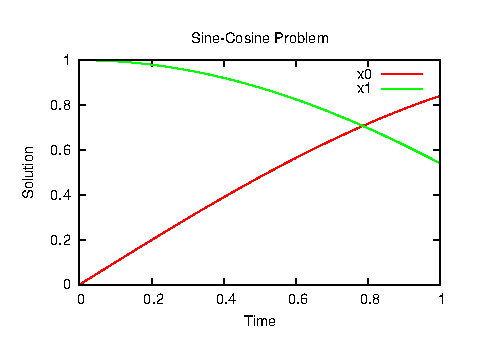
\includegraphics{figures/sincos}\caption{Exact solution to the Sine-Cosine problem.\label{rythmos:fig:SinCos-exact}}

\par\end{centering}

\end{figure}
Therefore this model has three model parameters and two initial conditions
which effect the exact solution as above. 
\[
\mathbf{p}=(a,f,L)
\]
\[
\dot{\mathbf{x}}=\mathbf{F}(\mathbf{x},t,\mathbf{p})
\]
where
\begin{eqnarray*}
F_{0} & = & x_{1}\\
F_{1} & = & \left(\frac{f}{L}\right)^{2}(a-x_{0})
\end{eqnarray*}


The exact sensitivities, $\mathbf{s}=\partial\mathbf{x}/\partial\mathbf{p}$,
for the problem are specified as
\[
\mathbf{s}(t)=\left[\begin{array}{cc}
1 & 0\\
\left(\frac{b}{L}\right)t\,\cos\left(\left(\frac{f}{L}\right)t+\phi\right) & \left(\frac{b}{L}\right)\cos\left(\left(\frac{f}{L}\right)t+\phi\right)-\frac{b\, f\, t}{L^{2}}\sin\left(\left(\frac{f}{L}\right)t+\phi\right)\\
-\frac{b\, f\, t}{L^{2}}\cos\left(\left(\frac{f}{L}\right)t+\phi\right) & -\frac{b\, f}{L^{2}}\cos\left(\left(\frac{f}{L}\right)t+\phi\right)+\frac{b\, f^{2}\, t}{L^{3}}\sin\left(\left(\frac{f}{L}\right)t+\phi\right)
\end{array}\right]
\]
and for the default initial conditions, $\phi=0$ and $b=1$
\[
\mathbf{s}(t=0)=\left[\begin{array}{cc}
1 & 0\\
0 & \frac{b}{L}\\
0 & -\frac{f}{L^{2}}
\end{array}\right]
\]
The time differentiated sensitivities, $\dot{\mathbf{s}}=\partial\mathbf{s}/\partial t=\partial/\partial t(\partial\mathbf{x}/\partial\mathbf{p})=\partial/\partial\mathbf{p}(\partial\mathbf{x}/\partial t)$
are
\[
\dot{\mathbf{s}}(t)=\left[\begin{array}{cc}
0 & 0\\
\left(\frac{b}{L}\right)\cos\left(\left(\frac{f}{L}\right)t+\phi\right)-\frac{b\, f\, t}{L^{2}}\sin\left(\left(\frac{f}{L}\right)t+\phi\right) & -\frac{2b\, f}{L^{2}}\sin\left(\left(\frac{f}{L}\right)t+\phi\right)\left(\frac{b}{L}\right)-\frac{b\, f^{2}\, t}{L^{3}}\cos\left(\left(\frac{f}{L}\right)t+\phi\right)\\
-\frac{b\, f}{L^{2}}\cos\left(\left(\frac{f}{L}\right)t+\phi\right)+\frac{b\, f^{2}\, t}{L^{3}}\sin\left(\left(\frac{f}{L}\right)t+\phi\right) & \frac{2b\, f^{2}}{L^{3}}\sin\left(\left(\frac{f}{L}\right)t+\phi\right)+\frac{b\, f^{3}\, t}{L^{4}}\cos\left(\left(\frac{f}{L}\right)t+\phi\right)
\end{array}\right]
\]



\subsection{Log-Time Problem\label{rythmos:sec:Log-Time-Problem}}

This problem was generated to be similar to those seen in Charon.
What is different about this solution is that it evolves on logarithmic
scale. As seen in Fig.~\ref{rythmos:fig:LogTime-exact}, the solution
has a very sharp gradient near $t=10^{-9}$ and then decays over many
order of magnitude until near constant at $t=1$.
\begin{figure}
\centering{}%
\begin{tabular}{cc}
a)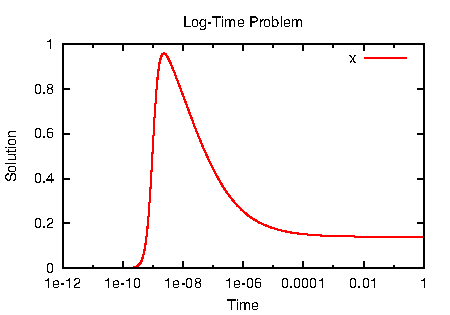
\includegraphics[width=2.75in]{figures/logtime-log} & b)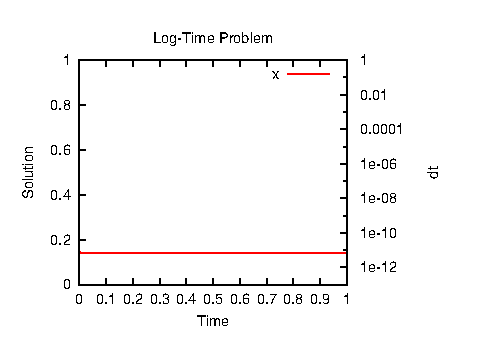
\includegraphics[width=2.75in]{figures/logtime-linear}\tabularnewline
\end{tabular}\caption{Exact solution to the Log-Time problem with a) logarithmic x-axis
and b) linear x-axis.\label{rythmos:fig:LogTime-exact}}
\end{figure}
From Fig.~\ref{rythmos:fig:LogTime-exact}, one can see the challenge
to capture the strong transient for $10^{-10}\leq t<10^{-8}$ requiring
step sizes at least as small as $\Delta t=10^{-11}$, and then transition
to larger and larger time steps as $t\rightarrow1$ to reduce the
overall computational costs.

The ODE for this problem is
\[
x(t)=\frac{a\left(bt^{4}+ct^{9/2}\right)}{\left(b+\sqrt{t}\right)\left(d+t^{4}\right)}
\]
where $a=1.4$, $b=0.0001$, $c=0.1$, $d=10^{-36}$, and the initial
condition is $x(0)=0.$ The center of the rapid increase is approximately
$d^{1/4}$, the product $ac$ sets the steady state value, and the
center of the decay is approximately $b^{2}$. The time derivative
is given by
\[
\dot{x}=\frac{at^{3}\left(8b^{2}d+b\sqrt{t}\left((9c+7)d+(c-1)t^{4}\right)+8cdt\right)}{2\left(b+\sqrt{t}\right)^{2}\left(d+t^{4}\right)^{2}}.
\]



\newpage{}


\part{Developer's Guide}


\section{Introduction}

The primary purpose of the Developer's Guide is to provide the high-level
OO design and description of the C++ interfaces and concrete implementations
for the solution of a broad class of transient ordinary differential
equations (ODEs) and differential algebraic equations (DAEs) in a
consistent manner. Although Doxygen is a good tool to explore the
details of the C++ interfaces and classes, it rarely provides the
high-level interaction of these objects and how they are intended
to be used. Therefore in this Developer's Guide, the high-level description
is given in order for new Rythmos developers can get the basic design
of Rythmos. It is intended that this description should remain fairly
stable over time, and not require many updates. However detailed information,
which could change more often, is left to the Doxygen webpages, which
obviously provides quick and easy document generation of software
implementation.

\begin{figure}
\centering{}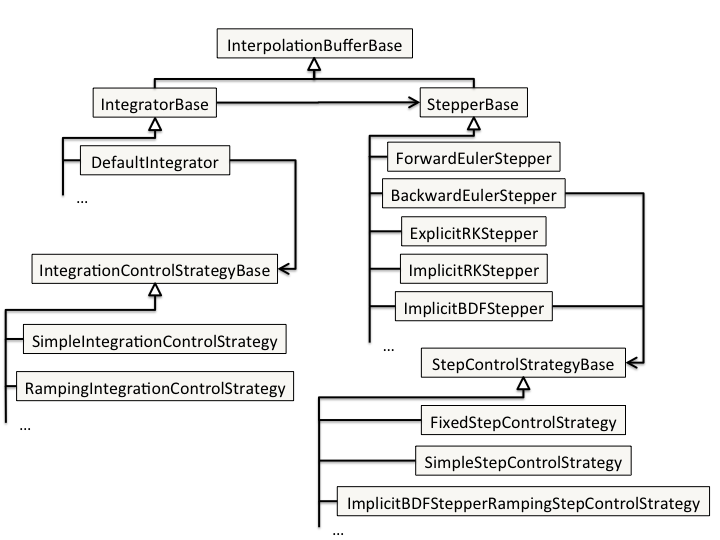
\includegraphics[width=5in]{figures/IntegratorStepperDesign}\caption{General relationships between the Integrators, IntegrationControlStrategies,
Steppers and StepControlStrategies.\label{rythmos:fig:IntegratorStepperDesign}}
\end{figure}



\subsection{Interpolation-Buffer Base\label{rythmos:sec:InterpolationBufferBase}}

An InterpolationBuffer is basically a container of solutions and time
derivatives (``states'') at discrete times (``time nodes'') over
a time range in ascending order, and can be used for storing checkpoints
and breakpoints of the state for later use. With an Interpolator specified,
a state at desired ``time points'' can be returned over the time
range with an accuracy of the order of the Interpolator. See Fig~\ref{rythmos:fig:InterpolationBuffer}.
\begin{figure}


\begin{centering}
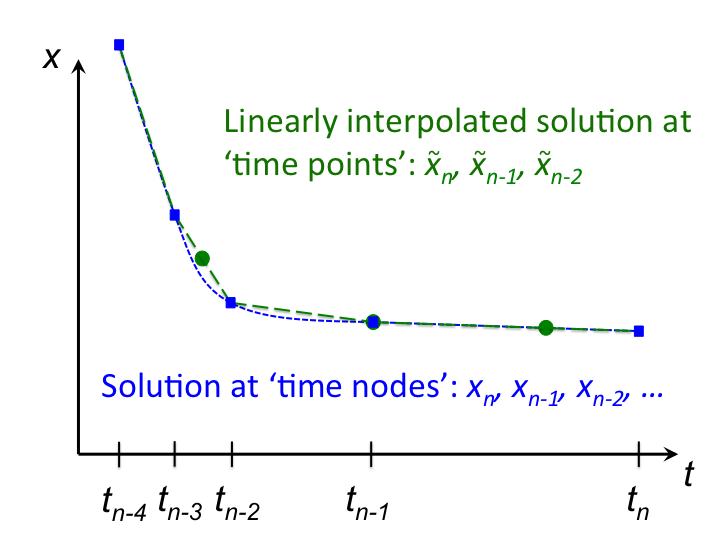
\includegraphics[width=4in]{figures/InterpolationBuffer}\caption{Illustrating the time points and time nodes in InterpolationBuffer
with a linear interpolator.\label{rythmos:fig:InterpolationBuffer}}

\par\end{centering}

\end{figure}


Part of the design here is to separate the state information (solutions
and time derivatives) from how the state is integrated to that time.
This can be used when separate ODEs and DAEs with different time integrators
are advanced in time, and wish to share their states (e.g., forward
and adjoint states, and operator-split solutions). No direct synchronizing
of time steps is required between them; time steps of each state can
be interpolated between for each integrator. 

An important caveat here is that the interpolated solutions are not
guaranteed to satisfy the ODE/DAE at the interpolated ``time points''.
This may be important for simulations where conservation is required,
e.g., conservation of mass, momentum and energy. The InterpolationBuffer
can be still useful in this situation, but the ``time nodes'' should
be used to ensure that the state satisfies the governing ODEs/DAEs.


\subsection{Integrator Base}

Time integration is carried out by Integrators, which inherit from
InterpolationBufferBase, and advance the state in time (step-by-step)
with Steppers. Integrators therefore have a set of states at given
times (see Sec.~\ref{rythmos:sec:InterpolationBufferBase}), and
can provide states to client requests. If the client requests a time
point within the current time range, the Integrator can simply return
an interpolated state. If the client requests a point forward in time,
the Integrator will advance the state to include the requested time.

The primary function of the Integrator is to manage the ``high-level''
time coordination required by the clients. Examples of this time marching
would include output of the solution state at various times, managing
checkpoints between solution states and adjoint states, coordinating
states between operator-split solutions, etc. All these coordinations
have very little to do with individual time steps, and more with times
where the solution states are required. This helps define the difference
between Integrators and Steppers when it comes to step-size selection
(Integration and Step Control Strategies).

In general the Integrator will request the largest step size required
to meet the next ``coordination'' (see Section~\ref{rythmos:sec:Integration-Control-Strategy}),
and leave the leave final determination of the step size to the Stepper
based on client specification, e.g., fixed or variable step size,
order, and accuracy (see Section~\ref{rythmos:sec:Step-Control-Strategy}).
Many times the step size completed by the Stepper will not advance
the state to the Integrator requested time, and the Integrator will
simply request another time step from the Stepper. With that said,
the Integrator has the flexibility to more directly control the time
stepping, and control the step size used by the Steppers. However
allowing the Stepper to choose the step size based on the Step Control
Strategy and having the Integration Control Strategy select ``coordination''
times is the preferred approach.


\subsection{Integration Control-Strategy\label{rythmos:sec:Integration-Control-Strategy}}

The Integration Control-Strategy is meant to determine the step size
needed for ``high-level'' simulation coordination (e.g., operator
splitting), solution output, and/or Stepper failure. In the Integration
Control-Strategy, we are not concerned with the accuracy of the solution,
as much as we are concerned with when are solutions needed. Obviously
one could control the Stepper step size with the Integration control-strategy
by using a \emph{fixed} step type and requiring the desired step size
be taken. This is especially useful for Steppers that can only handle
\emph{fixed} step types.


\subsection{Stepper Base}

A Stepper is a basic building block for DAE/ODE solvers. It advances
the state by ONE time step,
\[
x_{n-1}\underset{\Delta t}{\longrightarrow}x_{n},
\]
that has been requested by the Integrator. This time step can be fixed
or variable, where a \emph{fixed }step size indicates the stepper
will take the requested step size or fail, and where a \emph{variable}
step size allows the Stepper to adjust the step size to meet accuracy
and/or order requirements, and report to the Integrator the step size
taken. Most Steppers can be implemented very quickly for fixed step
sizes, and allow the Integrator to control the step size through an
Integration Control-Strategy (see Sec.~\ref{rythmos:sec:Integration-Control-Strategy}).
For variable step sizes, the Stepper needs a Step Control-Strategy
(see Sec.~\ref{rythmos:sec:Step-Control-Strategy}) in order to adjust
the step size based on error/order, and handle time step failures.


\subsection{Step Control-Strategy\label{rythmos:sec:Step-Control-Strategy}}

\begin{figure}
\centering{}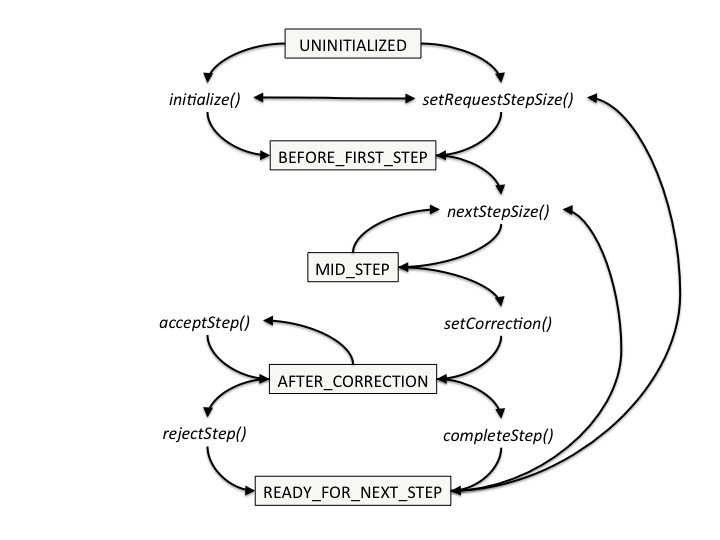
\includegraphics[width=5in]{figures/StepControlStrategy}\caption{Progression of the ControlStrategyState through a sequence of StepControlStrategy
functions by a Stepper.\label{rythmos:fig:StepControlStateProgression}}
\end{figure}
Step Control-Strategies are for adjusting the step size when a Stepper
is requested to take a variable step size by an Integrator. In order
to handle the correct progression of calls to Step Control-Strategies
functions (see Fig.~\ref{rythmos:fig:StepControlStateProgression}),
a ControlStrategyState is used, and can have the following values,
\texttt{\textsc{UNINITIALIZED}}, \texttt{\textsc{BEFORE\_FIRST\_STEP}},
\texttt{\textsc{MID\_STEP}}, \texttt{\textsc{AFTER\_CORRECTION}},
and \texttt{\textsc{READY\_FOR\_NEXT STEP}}.

The functions \emph{initialize()} and \emph{setRequestedStepsize()}
are used to prepare for the first step each time the Integrator calls
the Stepper, i.e., setting the requested step size and initializing
the Error Weight Vector. The \emph{nextStepsize() }function is used
to complete anything before starting the step. The \emph{setCorrection()}
functions is used to perform anything after the solver. i.e., the
correction. At this point the Stepper uses the StepControlStrategy
to determine if the step was acceptable with \emph{acceptStep(). }If
the step was acceptable, final computations of the solution and time
derivative are completed for the next time step by \emph{completeStep()}.
If the step was not acceptable, the step size and/order could be adjusted
by the StepControlStrategy function, \emph{rejectStep()}, and the
time step retried in order to obtain an acceptable time step. The\emph{
rejectStep()} function could completely reject the step and return
control to the Integrator to see if the Integrator Control Strategy
can do something to revive the time step.



\part{Back Matter}

\nocite{Gresho2000Vol1}

\nocite{Gresho2000Vol2}

\nocite{Hindmarsh2000}

\nocite{HairerNorsettWanner}

\nocite{GottliebShu1998}

\nocite{Kama2009}
\newpage{}

\printindex{}

\newpage{}

\bibliographystyle{plain}
\bibliography{RythmosTheory,../design_document/RythmosDesignSAND}

\end{document}
